
\newpage

\begin{flushright}
  \vspace{10cm}
  \rule{18cm}{5pt}
  \rule{18cm}{2pt}\vskip1cm
  \begin{center}
    \begin{bfseries}
      \Huge{\textbf{Build an event-driven serverless application using AWS Lambda}}\\
    \end{bfseries}
  \end{center}
  \vspace{1cm}
  \rule{18cm}{2pt}
  \rule{18cm}{5pt}
\end{flushright}
\newpage

\chapter{NOTE}
\section{Usage of AWS account}
On the account of Novelty, I attempted to create all the services required for this assignment, using the Serverless Framework[3]. Running this YAML file creates an IAM role for logging purposes.
Since I don't have permission to create an IAM role in the AWS academy account, I have used my personal AWS account to deploy the services for this entire assignment.

\chapter{Procedure followed for the given experiment}
    \section{AWS Architecture diagram}


    \begin{figure}[htp]
        \centering
        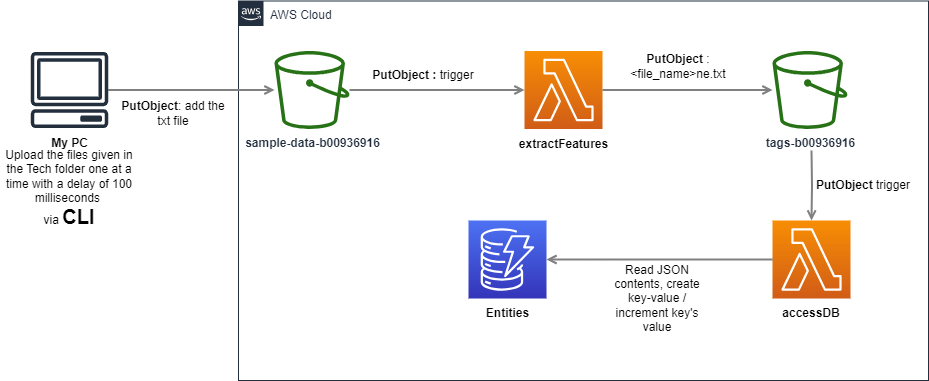
\includegraphics[scale=1, width=15cm]{PROBLEM 2/Screenshots/SDP-A3-Part B - Flowchart.png}
        \caption{\textbf{\textit{AWS Architecture diagram for the given work flow (Created using: draw.io [23])}}}
        \label{fig:aws-arch-diag}
    \end{figure}
    \section{Steps}
    \begin{enumerate}
        \item Configure the AWS credentials in the CLI using the command \textbf{"aws configure"}.
        \item Create an IAM role with the following permission provided by AWS, Role\_Name = \textbf{lambdaRole}: [21]
        \begin{enumerate}
            \item AWSLambdaExecute: Full access to CloudWatch Logs; Read, Write access to S3
        \end{enumerate}  
        \item Create an IAM role with the following permissions provided by AWS, Role\_Name = \textbf{lambdaRole\_accessDB}: [21]
        \begin{enumerate}
            \item AWSLambdaExecute: Full access to CloudWatch Logs; Read, Write access to S3
            \item AmazonDynamoDBFullAccess (as the name suggests)
        \end{enumerate}  
        \item Role = lambdaRole is for lambda extractFeatures
        \item Role = lambdaRole\_accessDB is for lambda accessDB
        
        \item Run the following command to create a serverless-framework project
    % Define custom colors for syntax highlighting
\definecolor{keyword}{RGB}{0, 0, 255}      % Blue for keywords
\definecolor{string}{RGB}{163, 21, 21}    % Red for strings
\definecolor{comment}{RGB}{0, 128, 0}     % Green for comments

\lstdefinelanguage{Serverless}{
  keywords={serverless, create, --template, aws-nodejs, --path},
  keywordstyle=\color{keyword}\bfseries,
  sensitive=false,
  morestring=[b]',
  morestring=[b]",
}


\begin{mdframed}[linewidth=1pt]
\lstset{
  language=Serverless,
  basicstyle=\ttfamily\small,
  commentstyle=\color{comment}\itshape,
  breaklines=true,
}
\begin{lstlisting}
# Create a new AWS Python3 Serverless project at path 'event-driven-serverless-app-a3'.
serverless create --template aws-python3 --path event-driven-serverless-app-a3
\end{lstlisting}
\end{mdframed}

\item Create the required resources using the following serverless framework script[3] (serverless.yml)[4] 



% Define custom colors for syntax highlighting
\definecolor{keyword}{RGB}{0, 0, 255}      % Blue for keywords
\definecolor{string}{RGB}{163, 21, 21}    % Red for strings
\definecolor{comment}{RGB}{0, 128, 0}     % Green for comments

% YAML language definition for listings package
\lstdefinelanguage{YAML}{
  keywords={service, provider, resources, Type, Properties, FunctionName, Code, Handler, Runtime, MemorySize, Timeout, Role, TableName, AttributeName, AttributeType, KeySchema, ProvisionedThroughput},
  keywordstyle=\color{keyword}\bfseries,
  sensitive=false,
  comment=[l]{\#},
  commentstyle=\color{comment}\ttfamily,
  stringstyle=\color{string}\ttfamily,
  morestring=[b]',
  morestring=[b]"
}


\begin{mdframed}[linewidth=1pt]
\lstset{language=YAML}
\begin{lstlisting}[basicstyle=\ttfamily\small, breaklines=true]
service: event-driven-serverless-app-a3

provider:
  name: aws
  runtime: python3.8
  stage: dev
  region: us-east-1

resources:
  Resources:
    # 1st S3 Bucket
    SampleDataBucket:
      Type: AWS::S3::Bucket
      Properties:
        BucketName: sample-data-b00936916 # Actual Bucket Name : SampleDataB00936916 -> Bucket name should not contain uppercase characters

    # 2nd S3 Bucket
    TagsBucket:
      Type: AWS::S3::Bucket
      Properties:
        BucketName: tags-b00936916 # Actual Bucket Name : TagsB00936916 -> Bucket name should not contain uppercase characters

    # Lambda Function to Extract Named Entities
    ExtractFeaturesLambda:
      Type: AWS::Lambda::Function
      Properties:
        FunctionName: extractFeatures
        Code:
          ZipFile: | #sample code
            def lambda_handler(event, context):
            # TODO implement
              return {
                'statusCode': 200,
                'body': json.dumps('Hello from Lambda!')
              }
        Handler: app.lambda_handler
        Runtime: python3.8   # Specify the runtime for the Lambda function
        MemorySize: 512
        Timeout: 10
        Role: arn:aws:iam::000966082997:role/lambdaRole #role with permissions : AWSLambdaExecute, AmazonDynamoDBFullAccess

    # Lambda Function to Access DynamoDB and Update
    AccessDBLambda:
      Type: AWS::Lambda::Function
      Properties:
        FunctionName: accessDB
        Code:
          ZipFile: | #sample code
            def lambda_handler(event, context):
            # TODO implement
              return {
                'statusCode': 200,
                'body': json.dumps('Hello from Lambda!')
              }
        Handler: app.lambda_handler
        Runtime: python3.8   # Specify the runtime for the Lambda function
        MemorySize: 512
        Timeout: 10
        Role: arn:aws:iam::000966082997:role/lambdaRole_accessDB #role with permissions : AWSLambdaExecute, AmazonDynamoDBFullAccess

    # DynamoDB Table
    DynamoDBTable:
      Type: AWS::DynamoDB::Table
      Properties:
        TableName: Entities
        AttributeDefinitions:
          - AttributeName: entity_name
            AttributeType: S # Set the AttributeType to String for the partition key "entity_name"
        KeySchema:
          - AttributeName: entity_name # Use file_name as the partition key
            KeyType: HASH  # Set the KeyType to HASH for the partition key "entity_name"
        ProvisionedThroughput:
          ReadCapacityUnits: 1
          WriteCapacityUnits: 1
\end{lstlisting}
\end{mdframed}

% \newpage
\item The above script does the following
\begin{enumerate}
    \item Create 2 - S3 buckets: sample-data-b00936916, tags-b00936916 
    \item Create 2 - lambdas: extractFeatures(with IAM role: lambdaRole), accessDB(with IAM role: lambdaRole\_accessDB)
    \item Create 1 - DynamoDB table: Entities (with Partition key: entity\_name)
\end{enumerate}

\item Run the command \textbf{serverless deploy} to deploy the .yml file to create the resources in CloudFormation 

        \item Run the following commands to \textbf{add the InvokeFunction permission} to both the lambdas \textbf{via} \textbf{CLI} [5]
        % Define custom colors for syntax highlighting
\definecolor{keyword}{RGB}{0, 0, 255}      % Blue for keywords
\definecolor{string}{RGB}{163, 21, 21}    % Red for strings
\definecolor{comment}{RGB}{0, 128, 0}     % Green for comments

% PowerShell language definition for listings package
\lstdefinelanguage{PowerShell}{
  keywords={aws, lambda, add-permission, --function-name, --action, --principal, --source-arn, --statement-id},
  keywordstyle=\color{keyword}\bfseries,
  sensitive=false,
  morestring=[b]',
  morestring=[b]",
}


\begin{mdframed}[linewidth=1pt]
\lstset{language=PowerShell}
\begin{lstlisting}[basicstyle=\ttfamily\small, breaklines=true]
Lambda_1:

Command = aws lambda add-permission --function-name arn:aws:lambda:us-east-1:000966082997:function:extractFeatures --action lambda:InvokeFunction --principal 000966082997 --source-arn arn:aws:s3:::sample-data-b00936916 --statement-id s3_trigger

Lambda_2:

Command = aws lambda add-permission --function-name arn:aws:lambda:us-east-1:000966082997:function:accessDB --action lambda:InvokeFunction --principal 000966082997 --source-arn arn:aws:s3:::tags-b00936916 --statement-id s3_trigger
\end{lstlisting}
\end{mdframed}

    \item Now, create separate JSON files with the below contents, to specify the LambdaFunctionConfigurations, to add S3 event notification.[7]
    \begin{enumerate}
        \item \textbf{sample-data-b00936916} bucket (trigger\_configuration\_sample-data-b00936916.json)
        % Define custom colors for syntax highlighting
\definecolor{keyword}{RGB}{0, 0, 255}      % Blue for keywords
\definecolor{string}{RGB}{163, 21, 21}    % Red for strings
\definecolor{comment}{RGB}{0, 128, 0}     % Green for comments

% JSON language definition for listings package
\lstdefinelanguage{json}{
  basicstyle=\ttfamily\small,
  keywordstyle=\color{keyword}\bfseries,
  commentstyle=\color{comment}\itshape,
  stringstyle=\color{string},
  morecomment=[l]{//},
  morecomment=[s]{/*}{*/},
  moredelim=[is][\color{blue}\bfseries]{\{}{\}},
  moredelim=[is][\color{blue}\bfseries]{[}{]},
  showstringspaces=false,
  breaklines=true
}


\begin{mdframed}[linewidth=1pt]
\lstset{language=json}
\begin{lstlisting}
{
{
  "LambdaFunctionConfigurations": [
    {
      "LambdaFunctionArn": "arn:aws:lambda:us-east-1:000966082997:function:extractFeatures",
      "Events": ["s3:ObjectCreated:*"]
    }
  ]
}
\end{lstlisting}
\end{mdframed}
      \item \textbf{tags-b00936916} bucket (trigger\_configuration\_tags-b00936916.json)
        % Define custom colors for syntax highlighting
\definecolor{keyword}{RGB}{0, 0, 255}      % Blue for keywords
\definecolor{string}{RGB}{163, 21, 21}    % Red for strings
\definecolor{comment}{RGB}{0, 128, 0}     % Green for comments

% JSON language definition for listings package
\lstdefinelanguage{json}{
  basicstyle=\ttfamily\small,
  keywordstyle=\color{keyword}\bfseries,
  commentstyle=\color{comment}\itshape,
  stringstyle=\color{string},
  morecomment=[l]{//},
  morecomment=[s]{/*}{*/},
  moredelim=[is][\color{blue}\bfseries]{\{}{\}},
  moredelim=[is][\color{blue}\bfseries]{[}{]},
  showstringspaces=false,
  breaklines=true
}


\begin{mdframed}[linewidth=1pt]
\lstset{language=json}
\begin{lstlisting}
{
{
    "LambdaFunctionConfigurations": [
      {
        "LambdaFunctionArn": "arn:aws:lambda:us-east-1:000966082997:function:accessDB",
        "Events": ["s3:ObjectCreated:*"]
      }
    ]
}
\end{lstlisting}
\end{mdframed}
    \end{enumerate}

    \item Now, run the following commands to add the S3 event notification to each bucket[11], \textbf{specifying the path} to the above created json file using \textbf{file://\textless /path/to/file_name\textgreater.json} [6]

% Define custom colors for syntax highlighting
\definecolor{keyword}{RGB}{0, 0, 255}      % Blue for keywords
\definecolor{string}{RGB}{163, 21, 21}    % Red for strings
\definecolor{comment}{RGB}{0, 128, 0}     % Green for comments

% PowerShell language definition for listings package
\lstdefinelanguage{PowerShell}{
  keywords={aws, lambda, add-permission, --function-name, --action, --principal, --source-arn, --statement-id},
  keywordstyle=\color{keyword}\bfseries,
  sensitive=false,
  morestring=[b]',
  morestring=[b]",
}


\begin{mdframed}[linewidth=1pt]
\lstset{language=PowerShell}
\begin{lstlisting}[basicstyle=\ttfamily\small, breaklines=true]
Bucket1:

Command = aws s3api put-bucket-notification-configuration --bucket sample-data-b00936916 --notification-configuration file://trigger_configuration_sample-data-b00936916.json


Bucket2:

Command = aws s3api put-bucket-notification-configuration --bucket tags-b00936916 --notification-configuration file://trigger_configuration_tags-b00936916.json
\end{lstlisting}
\end{mdframed}
    
    % \item Now, run the following commands in CLI to add an S3 trigger to each of the buckets.
    
        \item  Download the tech.zip file, extract it, change directory to folder 'tech' [22], open the terminal, run the following script[12]

        % Define custom colors for syntax highlighting
\definecolor{keyword}{RGB}{0, 0, 255}      % Blue for keywords
\definecolor{string}{RGB}{163, 21, 21}    % Red for strings
\definecolor{comment}{RGB}{0, 128, 0}     % Green for comments

% PowerShell language definition for listings package
\lstdefinelanguage{PowerShell}{
  keywords={foreach, in, Get-ChildItem, aws, s3, cp, Start-Sleep},
  keywordstyle=\color{keyword}\bfseries,
  sensitive=false,
  morestring=[b]',
  morestring=[b]",
}


\begin{mdframed}[linewidth=1pt]
\lstset{language=PowerShell}
\begin{lstlisting}[basicstyle=\ttfamily\small, breaklines=true]
foreach ($file in Get-ChildItem -File) {
    aws s3 cp "$file" s3://sample-data-b00936916/
    Start-Sleep -Milliseconds 100
}
\end{lstlisting}
\end{mdframed}

    \item Now, all the 401 files will be uploaded with a 100 milliseconds delay.
    \item Upon each upload, the flow of events mentioned in the architecture will be triggered, and all the names entities will be added to the 'Entities' dynamoDB databases, with the \textbf{key as the 'entity\_name' }and \textbf{value as its frequency}.
\end{enumerate}

\newpage
\section{Lamda code}
\subsection{extractFeatures}

% Define custom colors for syntax highlighting
\definecolor{keyword}{RGB}{0, 0, 255}      % Blue for keywords
\definecolor{string}{RGB}{163, 21, 21}    % Red for strings
\definecolor{comment}{RGB}{0, 128, 0}     % Green for comments

\lstdefinestyle{mystyle}{
    basicstyle=\ttfamily\small,
    keywordstyle=\color{keyword}\bfseries,
    commentstyle=\color{comment}\itshape,
    stringstyle=\color{string},
    showstringspaces=false,
    breaklines=true
}


\begin{mdframed}[linewidth=1pt]
\lstset{style=mystyle}
\begin{lstlisting}[language=Python]
import json
import re
import boto3

def lambda_handler(event, context):
    # Retrieve the S3 event information
    records = event['Records']
    for record in records:
        bucket = record['s3']['bucket']['name']
        key = record['s3']['object']['key']
        
        """
            Boto3 - Amazon Simple Storage Service (S3) API Documentation
            Reference: `Boto3 - Amazon S3 API <https://boto3.amazonaws.com/v1/documentation/api/latest/reference/services/s3.html>`_
        """

        # Read the contents of the file from S3
        s3_client = boto3.client('s3')
        response = s3_client.get_object(Bucket=bucket, Key=key)
        file_content = response['Body'].read().decode('utf-8')
        
        """
            Python Standard Library - re (Regular Expression) module
            Reference: `Python re (Regular Expression) module <https://docs.python.org/3/library/re.html>`_
        """

        # Extract words starting with a capital letter
        capital_words = re.findall(r'\b[A-Z][a-zA-Z]*\b', file_content)
        
        # Extract all caps words
        all_caps_words = re.findall(r'\b[A-Z]+\b', file_content)
        
        # Create a dictionary to store the named entities and their counts
        named_entities = {}
        
        # Count the occurrences of each word
        for word in capital_words + all_caps_words:
            named_entities[word] = named_entities.get(word, 0) + 1
        
        # Remove the file extension from the key
        file_name = key.split('.')[0]
        
        # Create the JSON object with the key as the file name and the named entities dictionary as the value
        result = {f"{file_name}ne": named_entities}
        
        # Convert the result to a JSON string
        named_entities_json = json.dumps(result)
        
        destination_s3_bucket = "tags-b00936916"

        # Upload the JSON to the tags-b00936916 bucket
        s3_client.put_object(Bucket=destination_s3_bucket, Key=f"{file_name}ne.txt", Body=named_entities_json)

    
    return {
        'statusCode': 200,
        'body': json.dumps('Named entities extracted successfully.')
    }


"""
All references:
    Python Standard Library - re (Regular Expression) module
    Reference: `Python re (Regular Expression) module <https://docs.python.org/3/library/re.html>`_

    Boto3 - Amazon Simple Storage Service (S3) API Documentation
    Reference: `Boto3 - Amazon S3 API <https://boto3.amazonaws.com/v1/documentation/api/latest/reference/services/s3.html>`_

"""
\end{lstlisting}
\end{mdframed}
% \newpage
\subsection{accessDB}

% Define custom colors for syntax highlighting
\definecolor{keyword}{RGB}{0, 0, 255}      % Blue for keywords
\definecolor{string}{RGB}{163, 21, 21}    % Red for strings
\definecolor{comment}{RGB}{0, 128, 0}     % Green for comments

\lstdefinestyle{mystyle}{
    basicstyle=\ttfamily\small,
    keywordstyle=\color{keyword}\bfseries,
    commentstyle=\color{comment}\itshape,
    stringstyle=\color{string},
    showstringspaces=false,
    breaklines=true
}


\begin{mdframed}[linewidth=1pt]
\lstset{style=mystyle}
\begin{lstlisting}[language=Python]
import json
import boto3

def lambda_handler(event, context):
    # Retrieve the S3 event information
    records = event['Records']
    for record in records:
        bucket = record['s3']['bucket']['name']
        key = record['s3']['object']['key']
        
        # Check if the file is in the format "001ne.txt"
        if key.endswith("ne.txt"):
            """
                Boto3 - Amazon Simple Storage Service (S3) API Documentation
                Reference: `Boto3 - Amazon S3 API <https://boto3.amazonaws.com/v1/documentation/api/latest/reference/services/s3.html>`_
            """
            # Read the contents of the file from S3            
            s3_client = boto3.client('s3')

            response = s3_client.get_object(Bucket=bucket, Key=key)
            file_content = response['Body'].read().decode('utf-8')
            
            # Convert the JSON content to a dictionary
            named_entities = json.loads(file_content)
            
            # Get the file name from the key (e.g., "001ne.txt" -> "001ne")
            file_name = key.split('.')[0]
            
            """
                Boto3 - Amazon DynamoDB API Documentation
                Reference: `Boto3 - Amazon DynamoDB API <https://boto3.amazonaws.com/v1/documentation/api/latest/reference/services/dynamodb.html>`_
            """
            # Update the DynamoDB table with the named entities
            dynamodb = boto3.resource('dynamodb')
            table = dynamodb.Table('Entities')
            
            for entity, count in named_entities[file_name].items():
                # Convert the count to an integer before updating the table
                count = int(count)
                # Update the table with the named entity and its count
                table.update_item(
                    Key={'entity_name': entity},
                    UpdateExpression='SET frequency = if_not_exists(frequency, :zero) + :val',
                    ExpressionAttributeValues={':zero': 0, ':val': count}
                )
                
    return {
        'statusCode': 200,
        'body': json.dumps('DynamoDB table updated successfully.')
    }



"""
All references:
    Boto3 - Amazon Simple Storage Service (S3) API Documentation
    Reference: `Boto3 - Amazon S3 API <https://boto3.amazonaws.com/v1/documentation/api/latest/reference/services/s3.html>`_

    Boto3 - Amazon DynamoDB API Documentation
    Reference: `Boto3 - Amazon DynamoDB API <https://boto3.amazonaws.com/v1/documentation/api/latest/reference/services/dynamodb.html>`_
"""

\end{lstlisting}
\end{mdframed}

% \newpage
\subsection{Screenshots}

\begin{figure}[htp]
    \centering
    \fbox{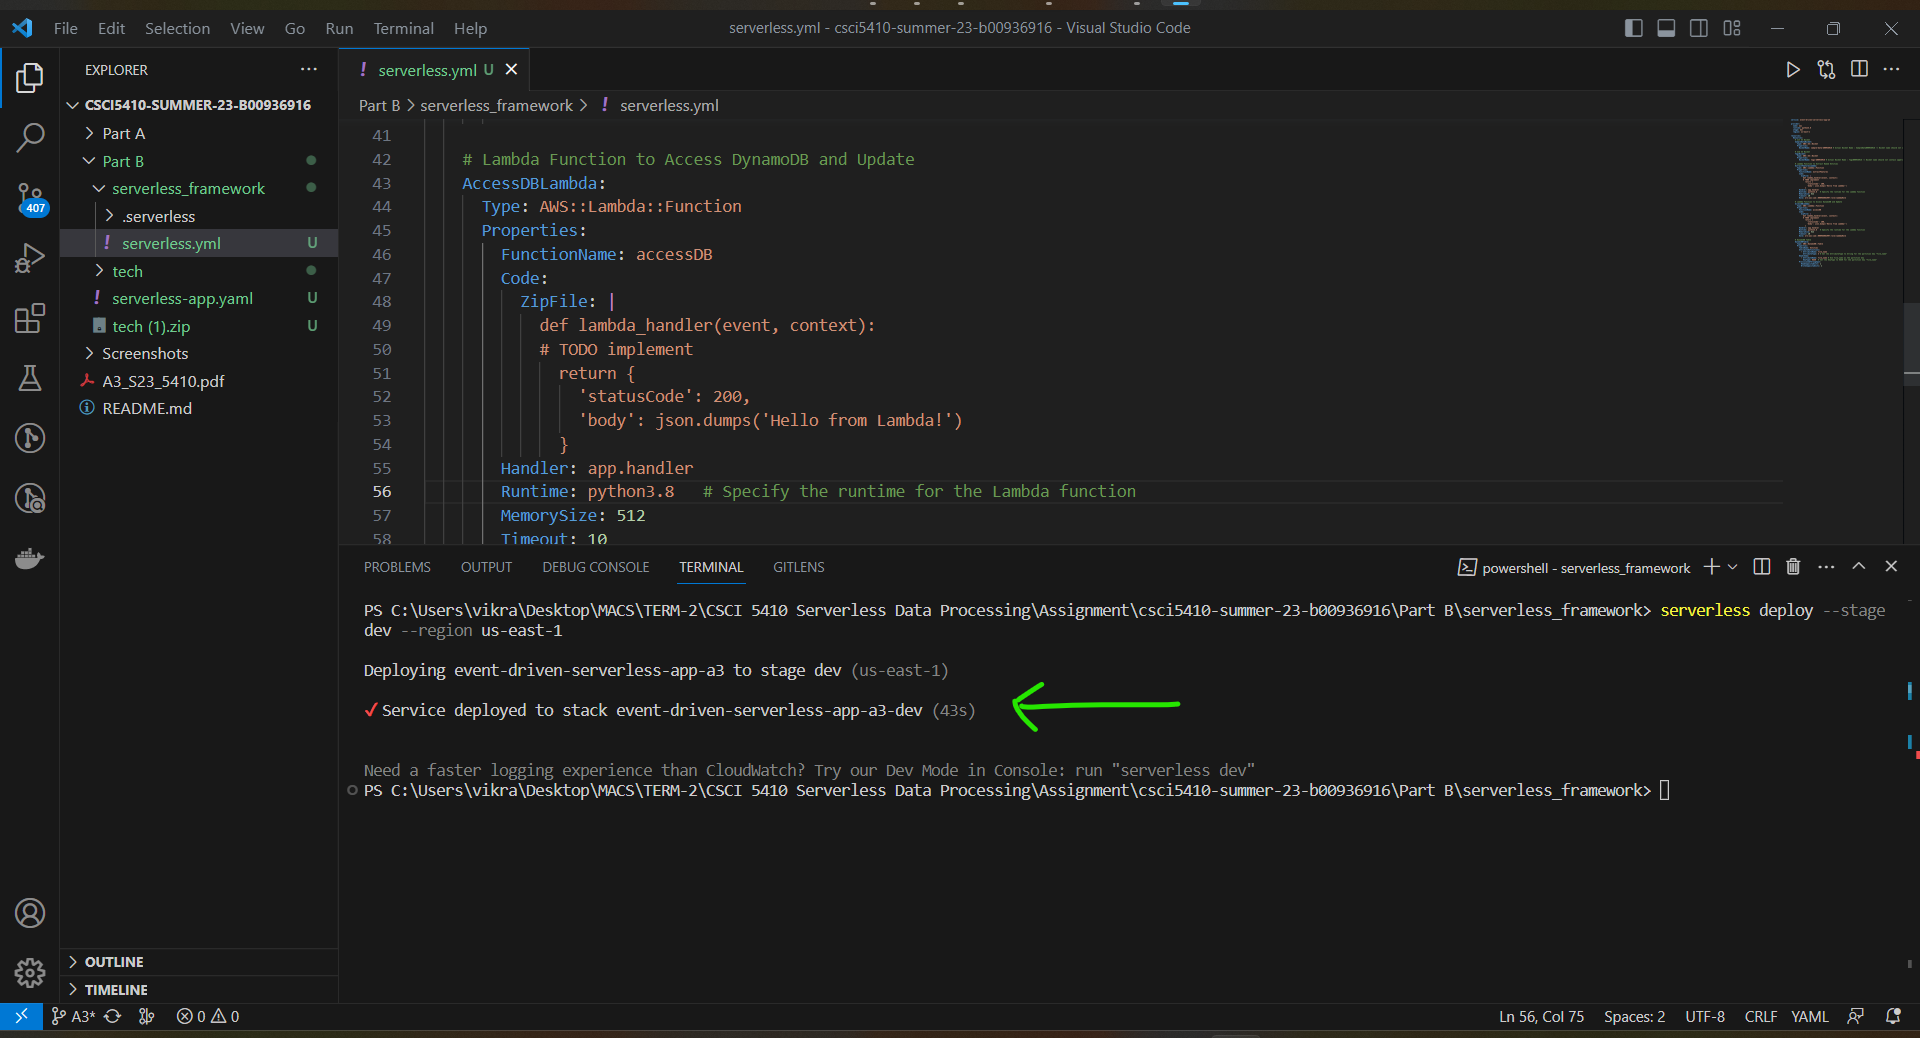
\includegraphics[scale=1, width=15cm,height=7.5cm]{PROBLEM 2/Screenshots/1. cloud formation - resources created - CLI.png}}
    \caption{\textbf{\textit{Running Serverless-Framework script in CLI }}}
    \label{fig:sls-cli}
\end{figure}

\begin{figure}[htp]
    \centering
    \fbox{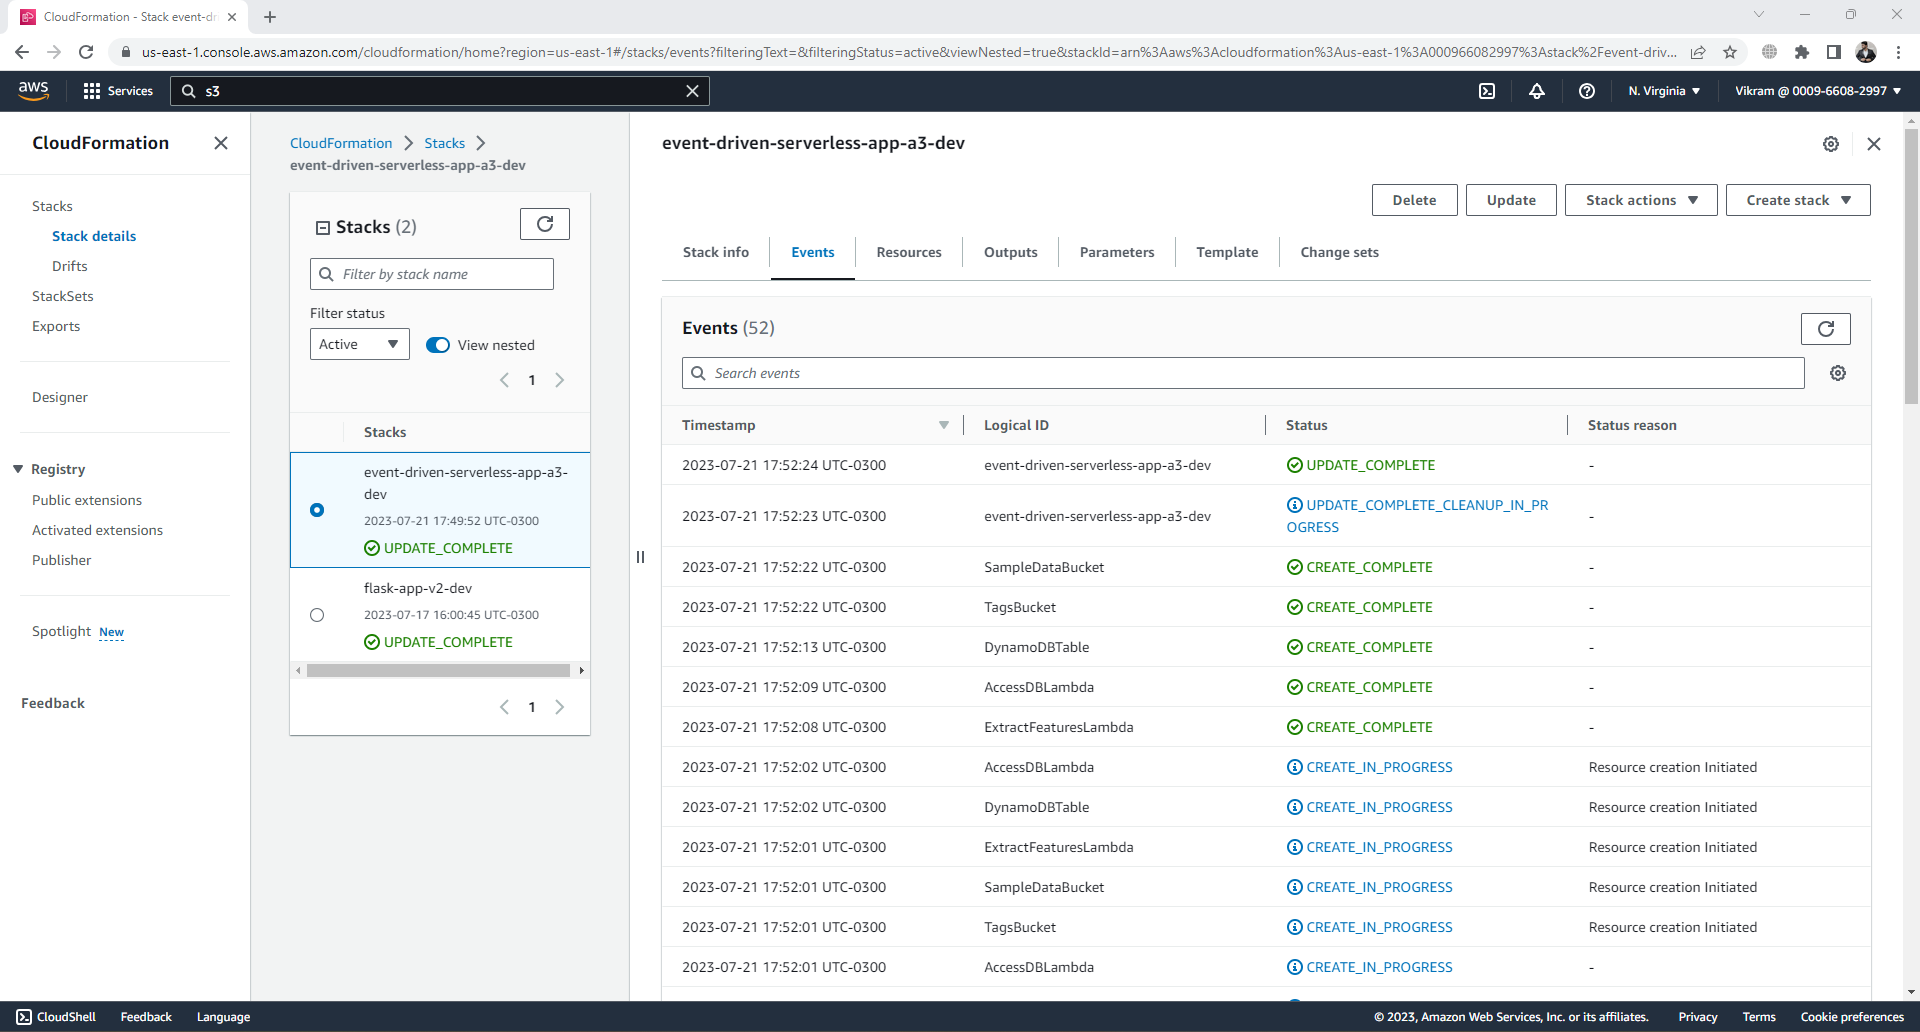
\includegraphics[scale=1, width=15cm,height=7.5cm]{PROBLEM 2/Screenshots/1.1 cloud formation - resources created - console.png}}
    \caption{\textbf{\textit{Resources stack created - CloudFormation in Console }}}
    \label{fig:}
\end{figure}

\begin{figure}[htp]
    \centering
    \fbox{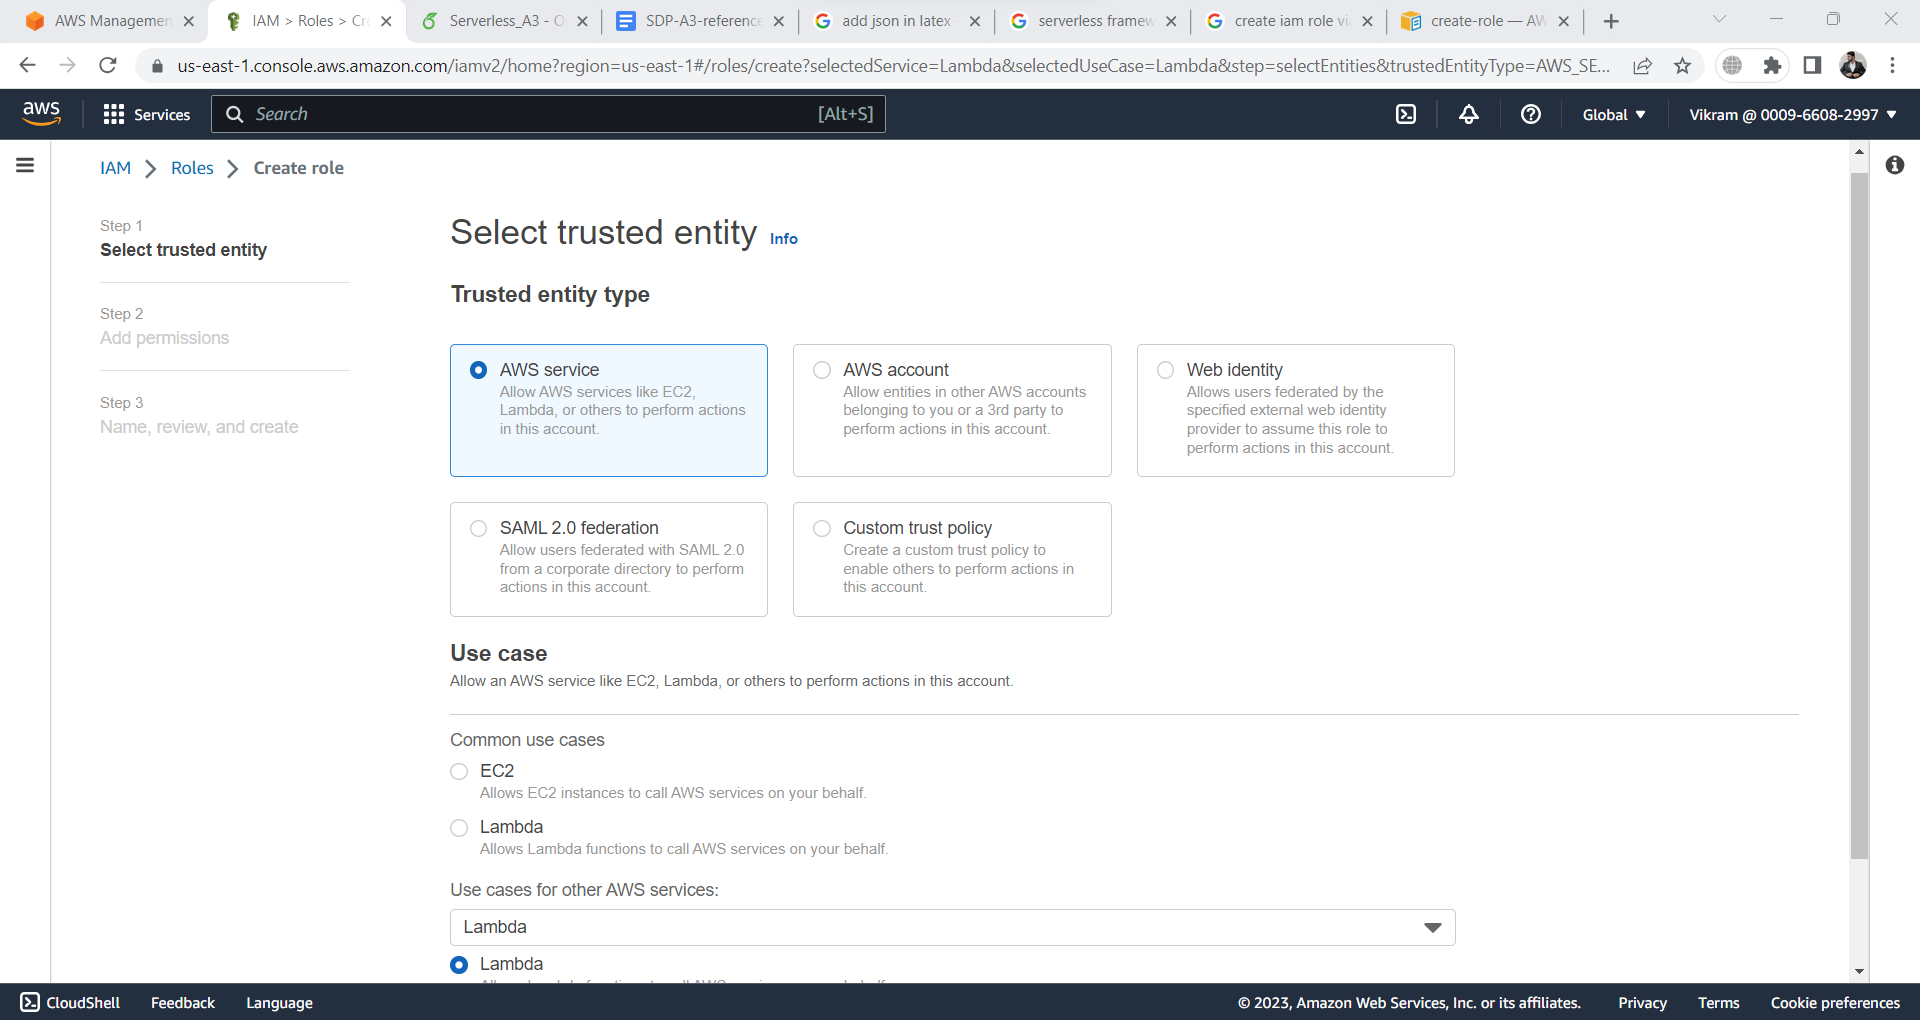
\includegraphics[scale=1, width=15cm,height=7.5cm]{PROBLEM 2/Screenshots/2.0.1 create lambda_1 role.png}}
    \caption{\textbf{\textit{Create IAM role for lambda extractFeatures}}}
    \label{fig:}
\end{figure}

\begin{figure}[htp]
    \centering
    \fbox{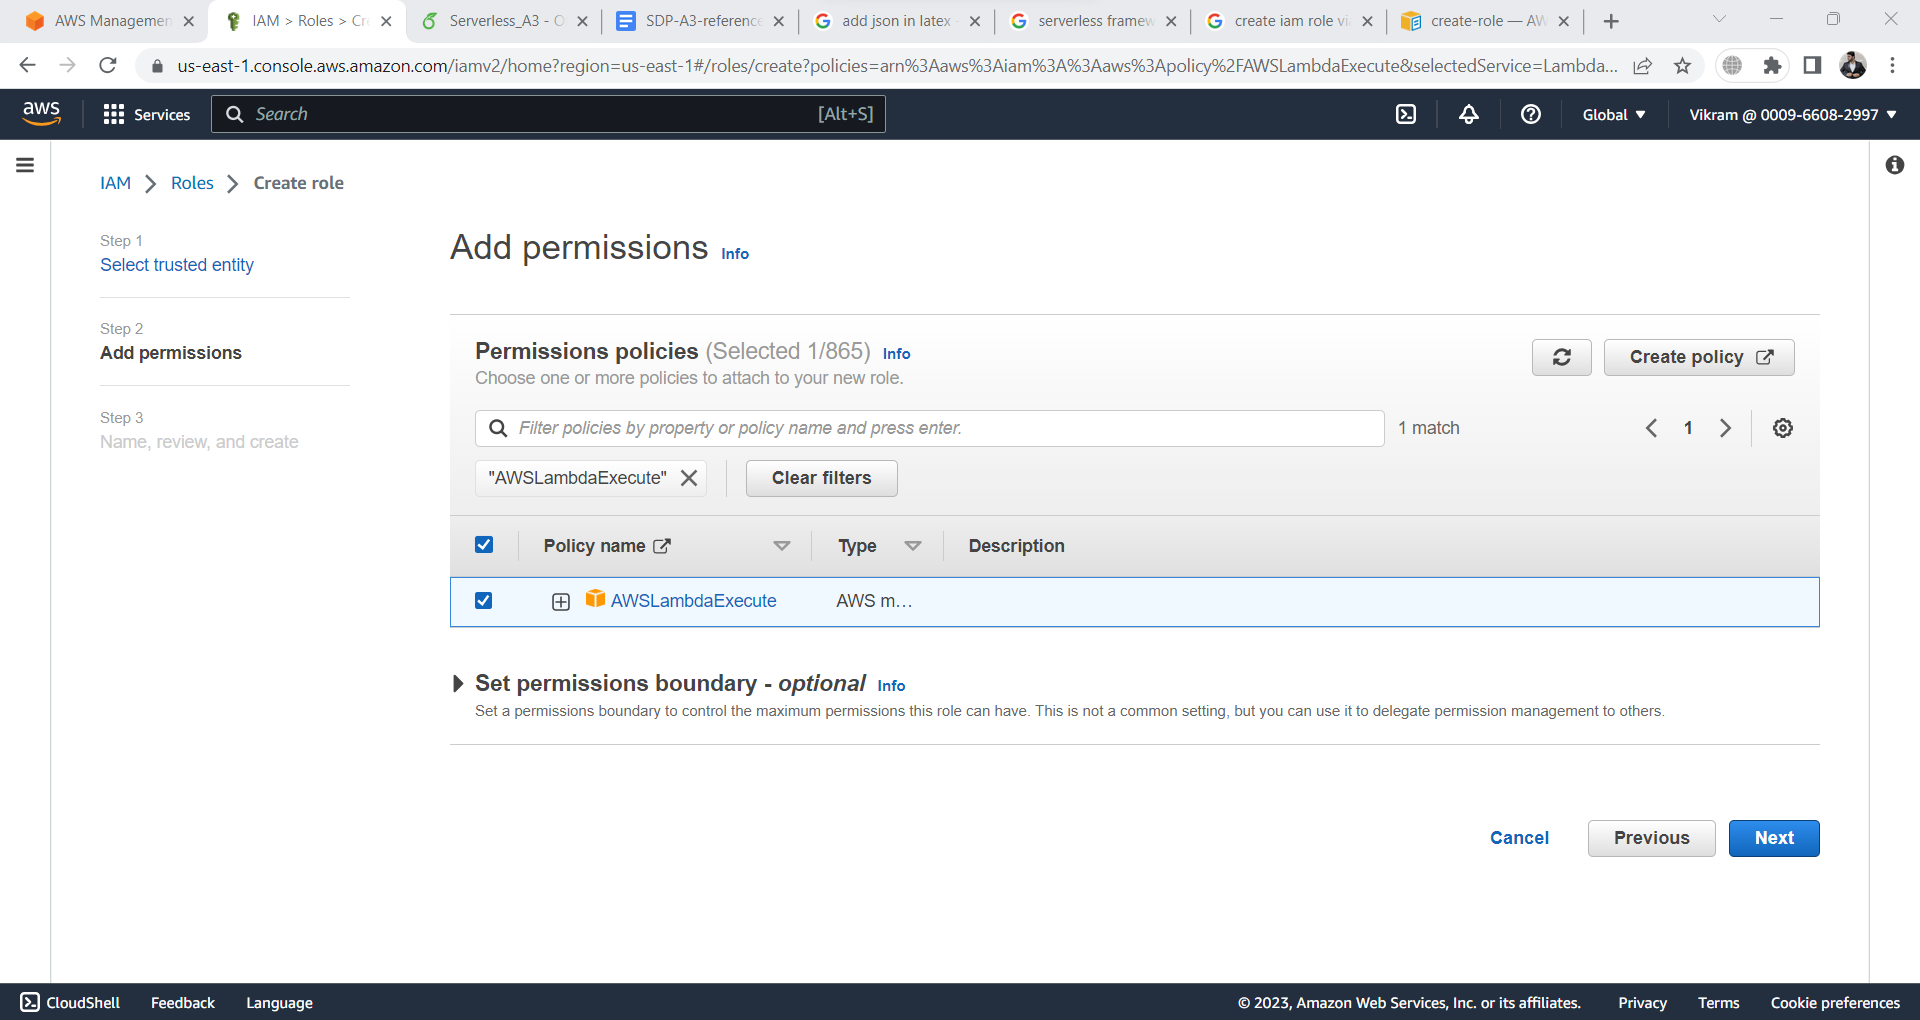
\includegraphics[scale=1, width=15cm,height=7.5cm]{PROBLEM 2/Screenshots/2.0.2 create lambda_1 role.png}}
    \caption{\textbf{\textit{Create IAM role for lambda extractFeatures}}}
    \label{fig:}
\end{figure}

\begin{figure}[htp]
    \centering
    \fbox{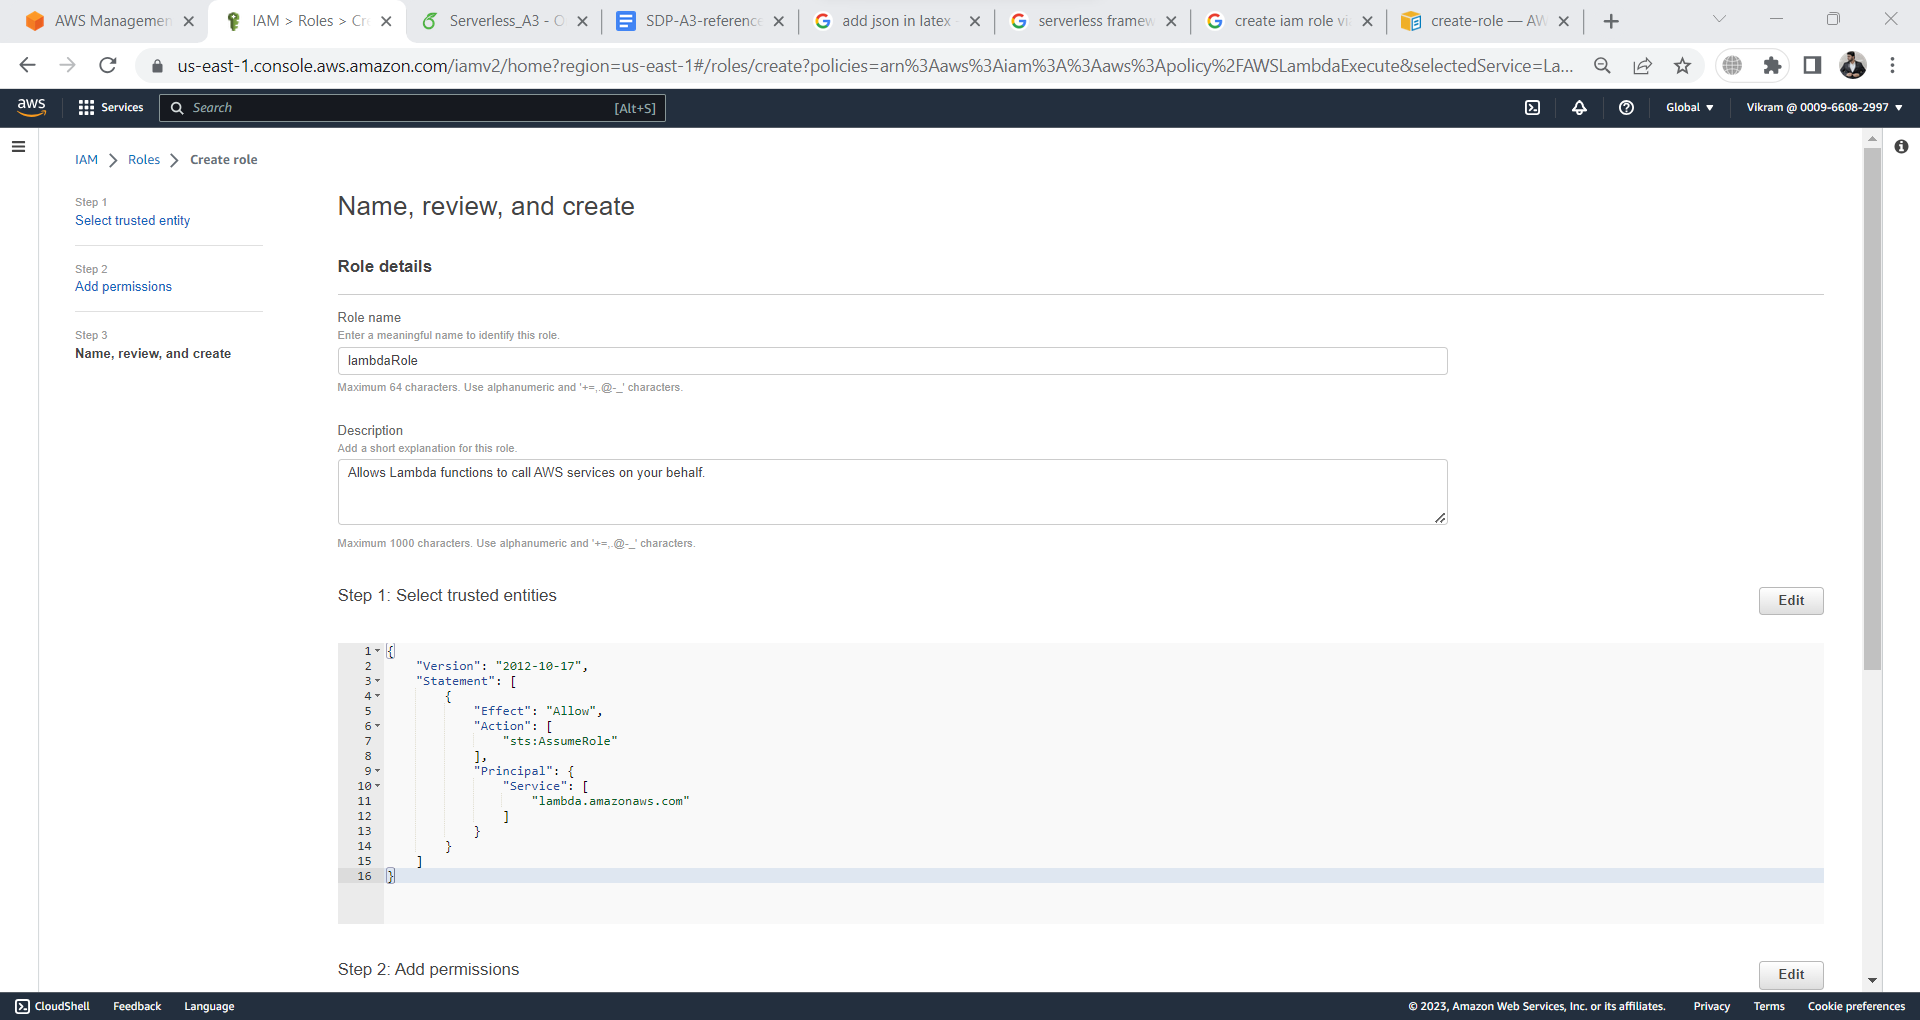
\includegraphics[scale=1, width=15cm,height=7.5cm]{PROBLEM 2/Screenshots/2.0.3 create lambda_1 role.png}}
    \caption{\textbf{\textit{Create IAM role for lambda extractFeatures}}}
    \label{fig:}
\end{figure}

\begin{figure}[htp]
    \centering
    \fbox{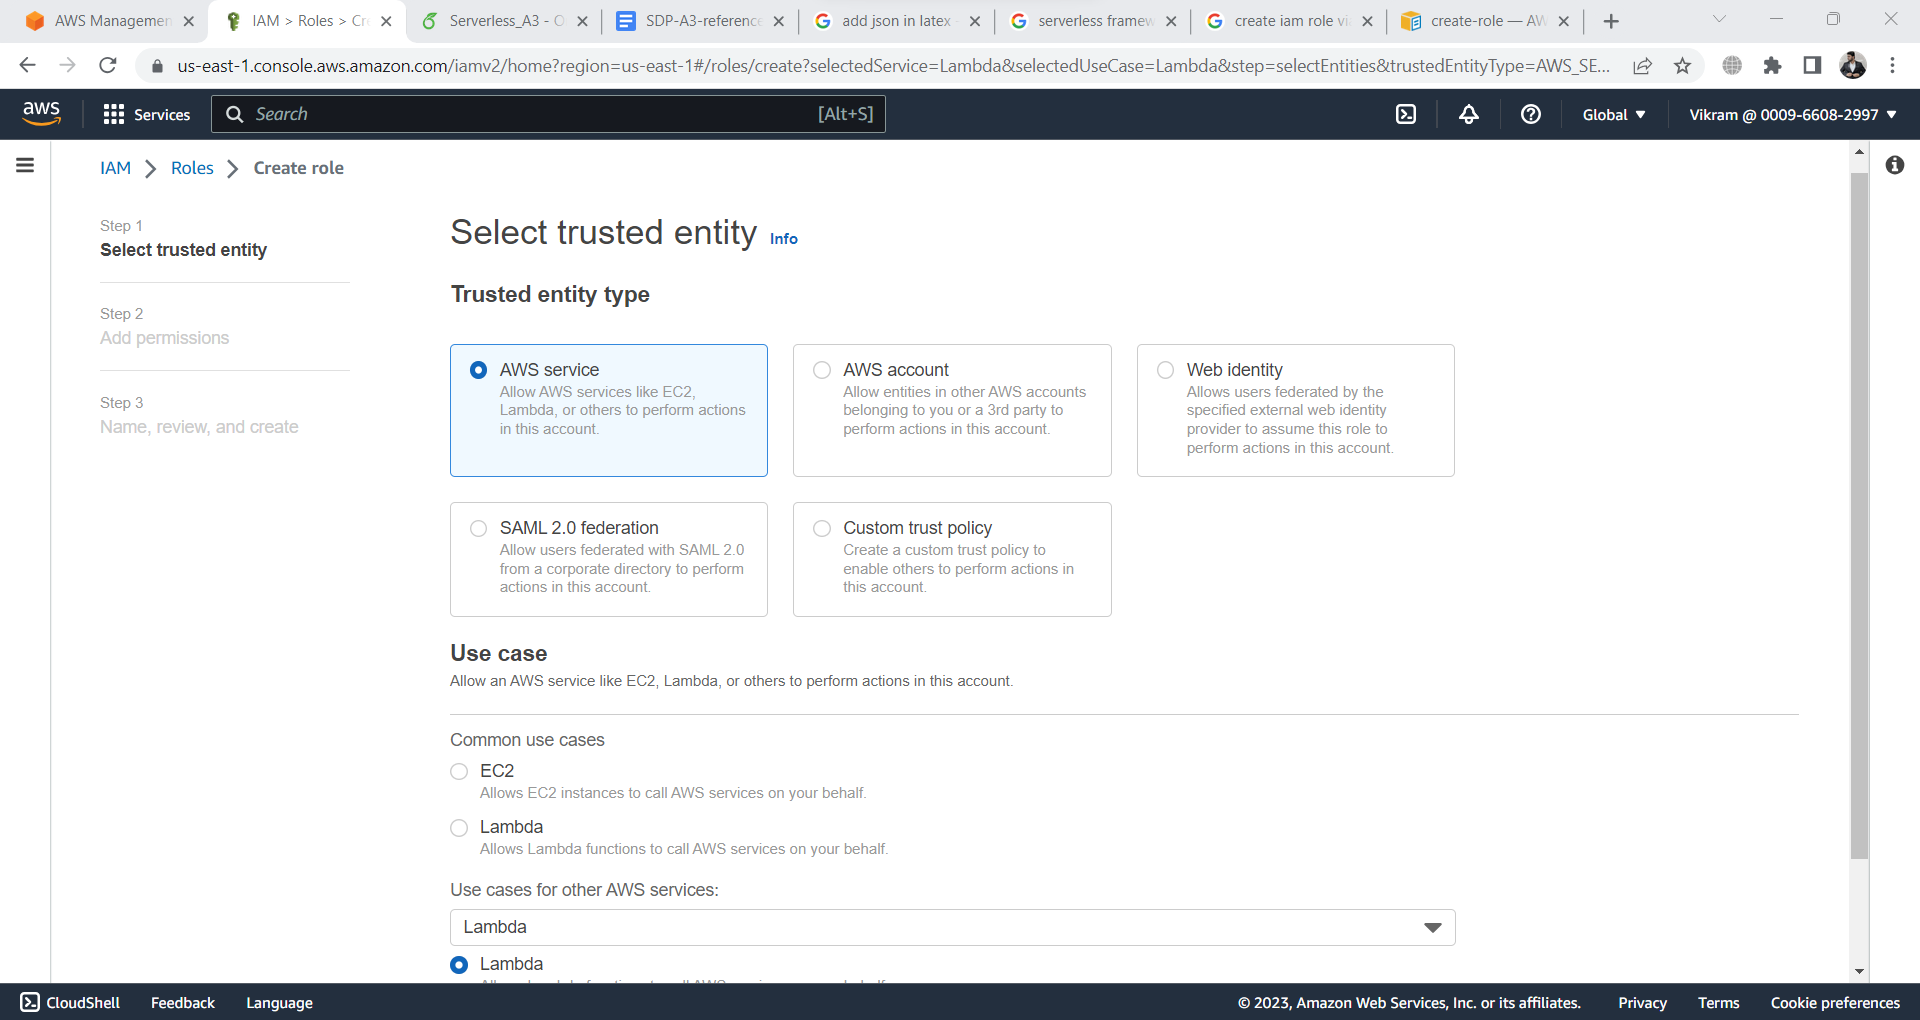
\includegraphics[scale=1, width=15cm,height=7.5cm]{PROBLEM 2/Screenshots/2.1 create lambda_2 role.png}}
    \caption{\textbf{\textit{Create IAM role for lambda accessDB}}}
    \label{fig:}
\end{figure}

\begin{figure}[htp]
    \centering
    \fbox{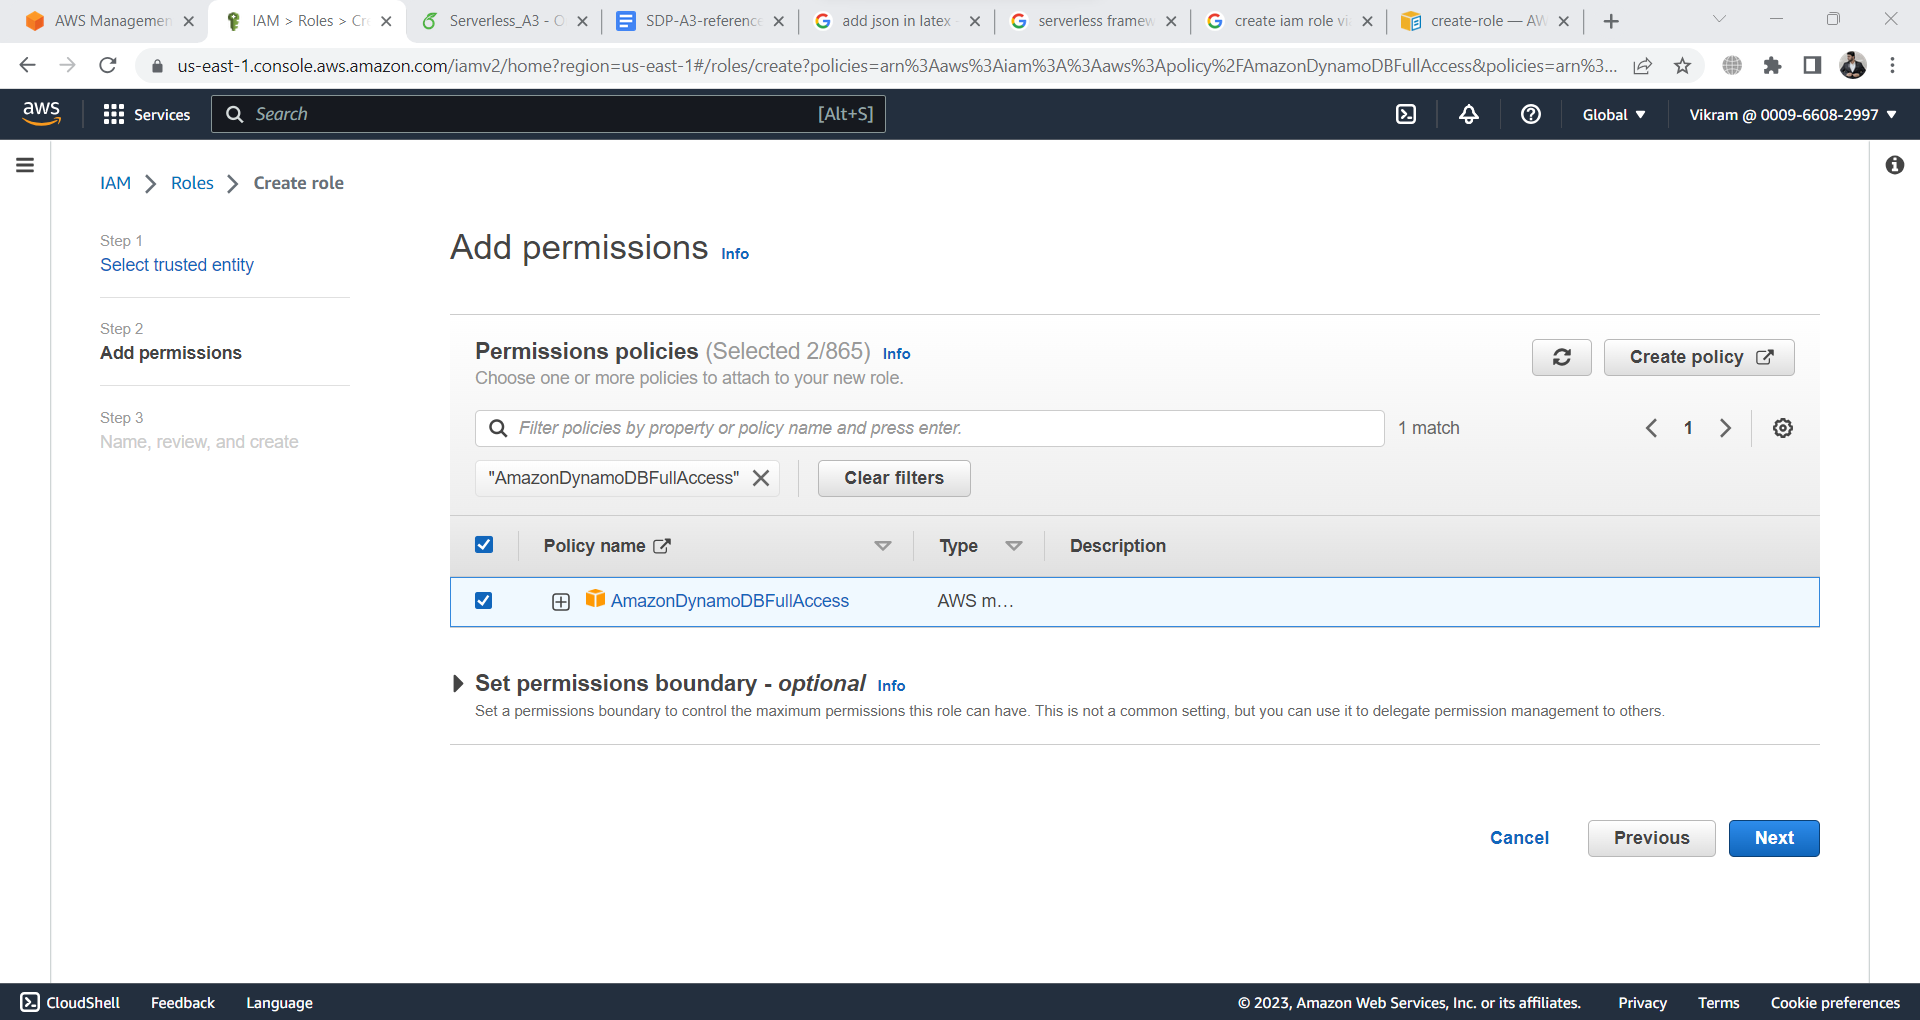
\includegraphics[scale=1, width=15cm,height=7.5cm]{PROBLEM 2/Screenshots/2.2 create lambda_2 role.png}}
    \caption{\textbf{\textit{Create IAM role for lambda accessDB}}}
    \label{fig:}
\end{figure}

\begin{figure}[htp]
    \centering
    \fbox{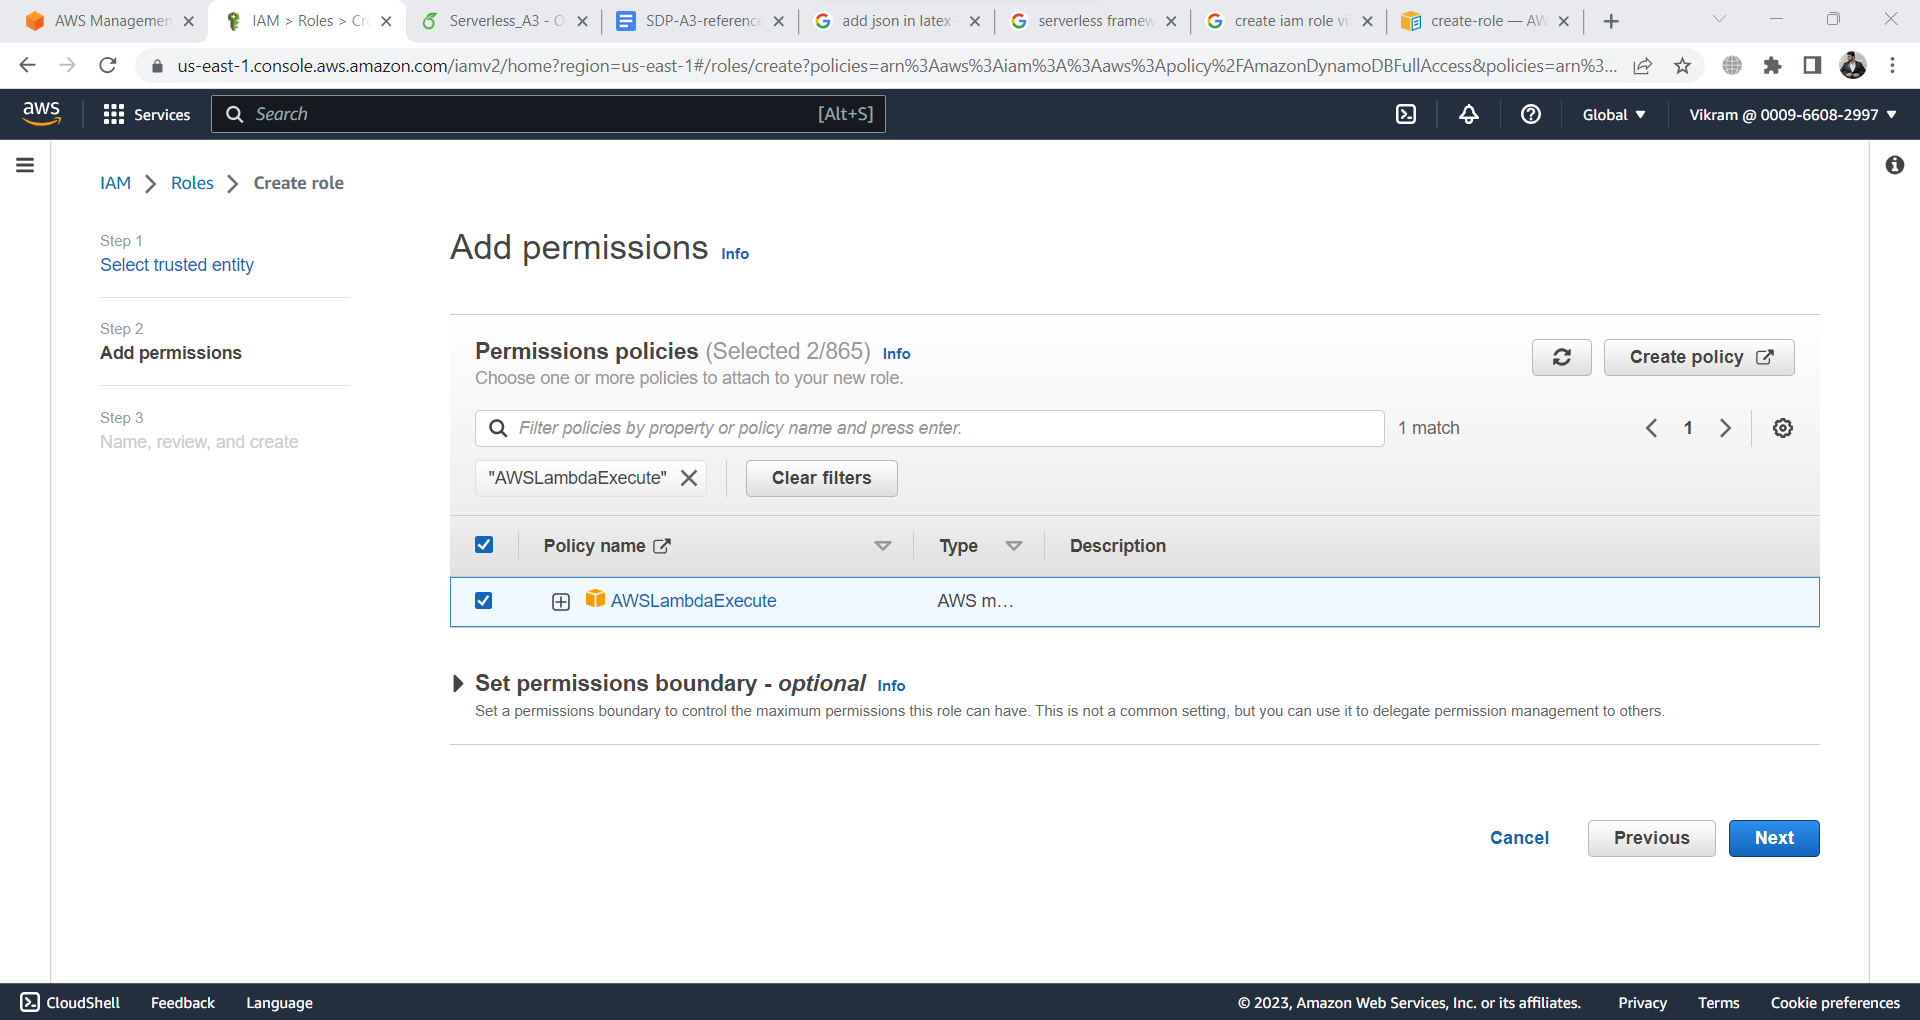
\includegraphics[scale=1, width=15cm,height=7.5cm]{PROBLEM 2/Screenshots/2.3 create lambda_2 role.png}}
    \caption{\textbf{\textit{Create IAM role for lambda accessDB}}}
    \label{fig:}
\end{figure}

\begin{figure}[htp]
    \centering
    \fbox{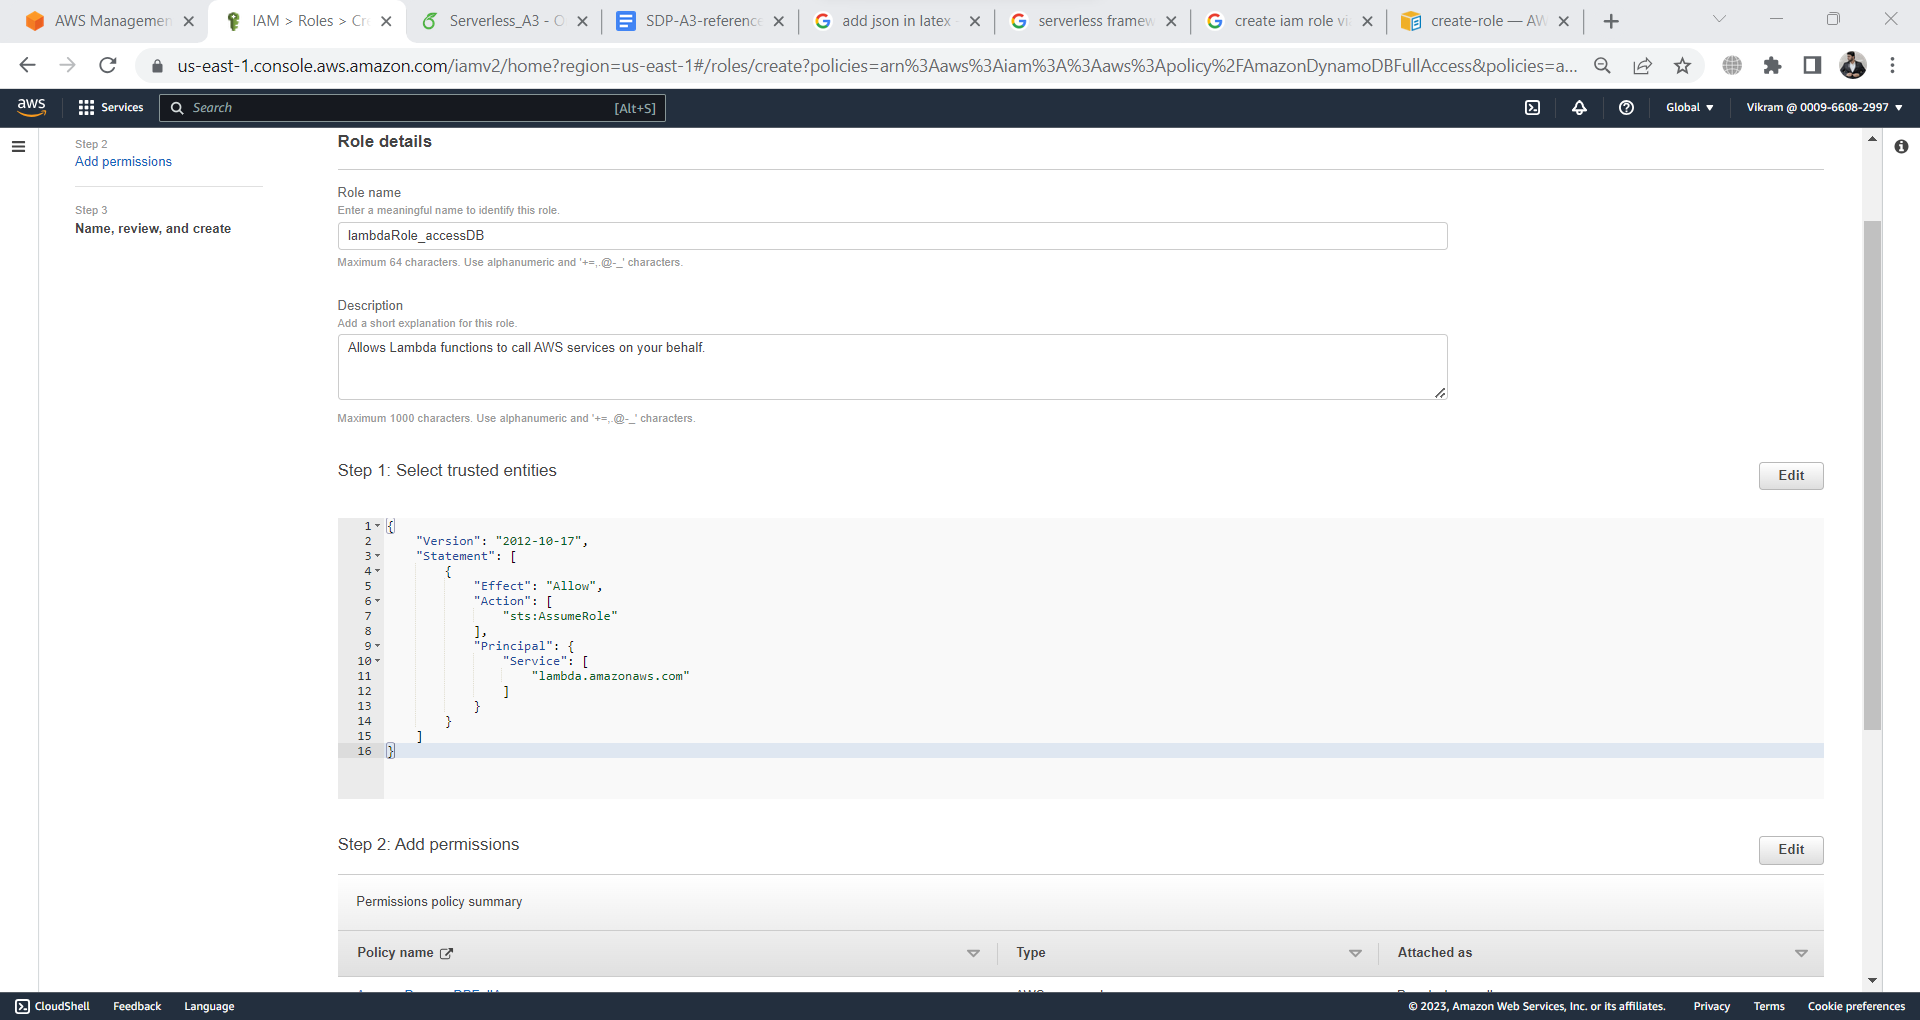
\includegraphics[scale=1, width=15cm,height=7.5cm]{PROBLEM 2/Screenshots/2.4 create lambda_2 role.png}}
    \caption{\textbf{\textit{Create IAM role for lambda accessDB}}}
    \label{fig:}
\end{figure}

\begin{figure}[htp]
    \centering
    \fbox{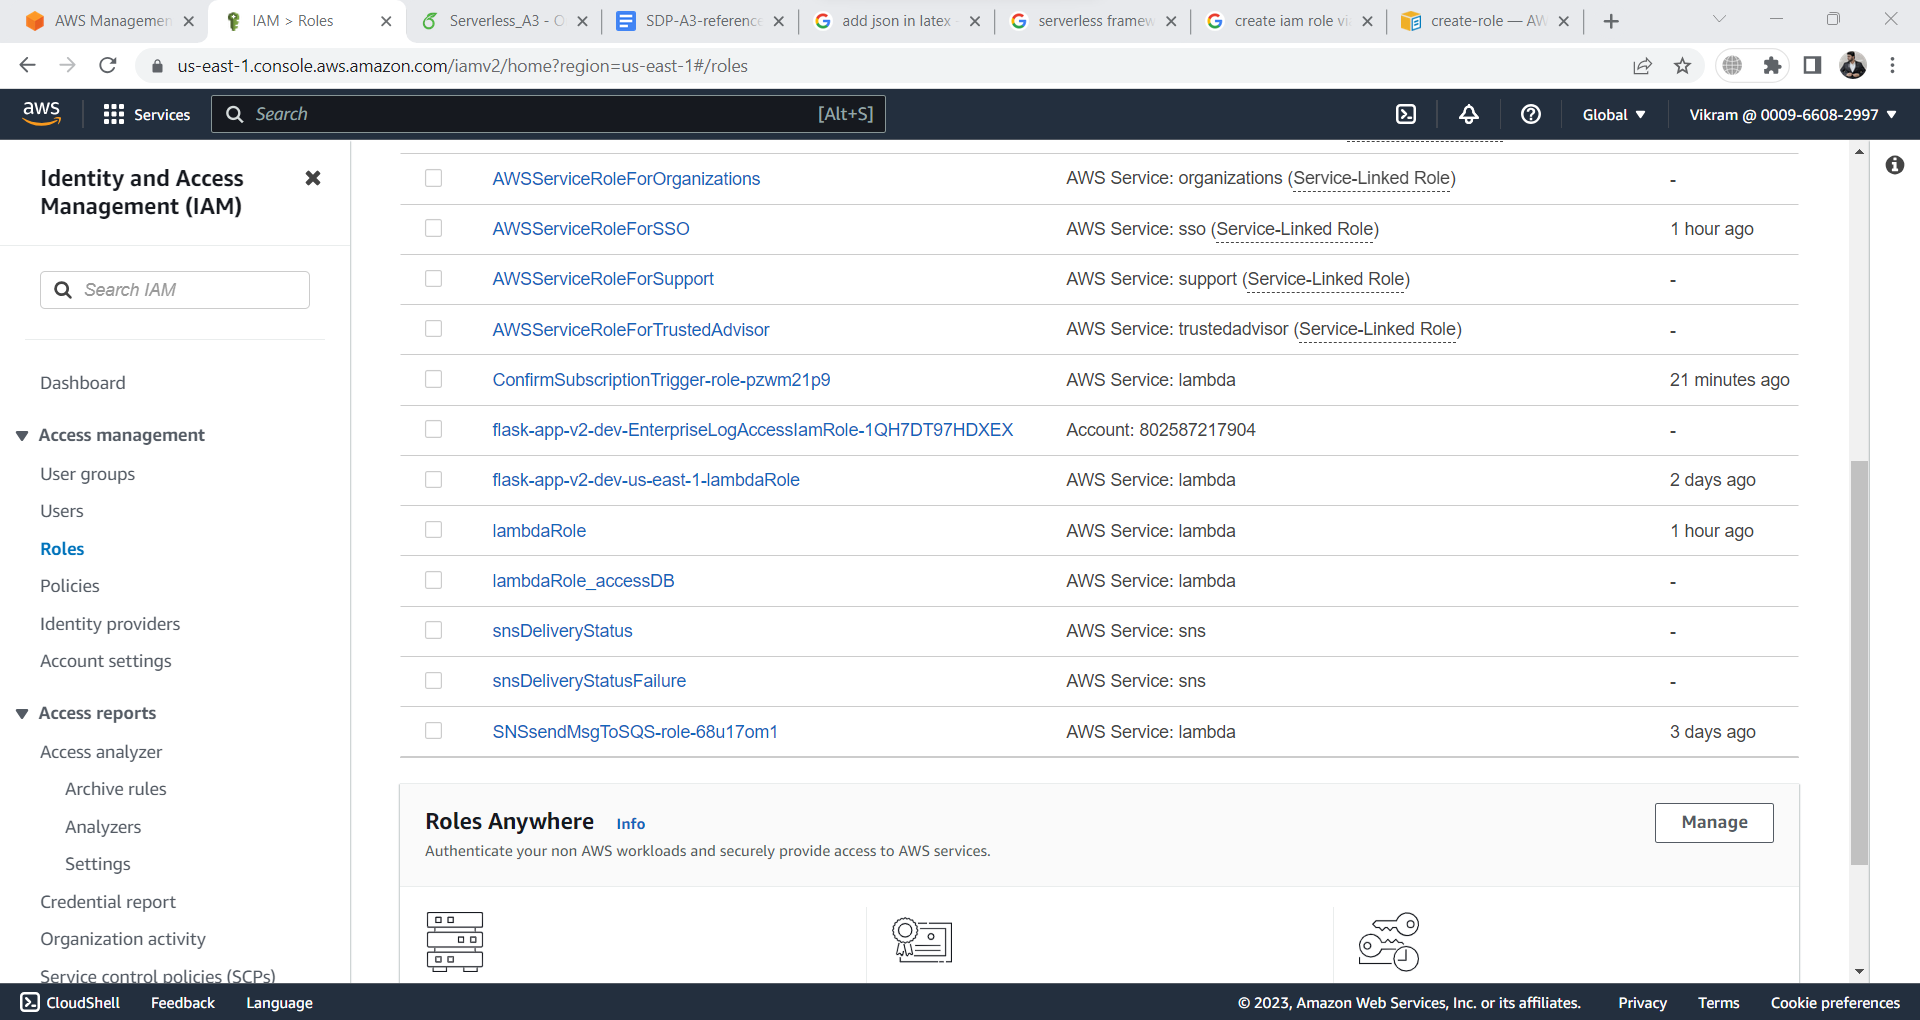
\includegraphics[scale=1, width=15cm,height=7.5cm]{PROBLEM 2/Screenshots/2.5 both roles created.png}}
    \caption{\textbf{\textit{Both the Roles created}}}
    \label{fig:}
\end{figure}

\begin{figure}[htp]
    \centering
    \fbox{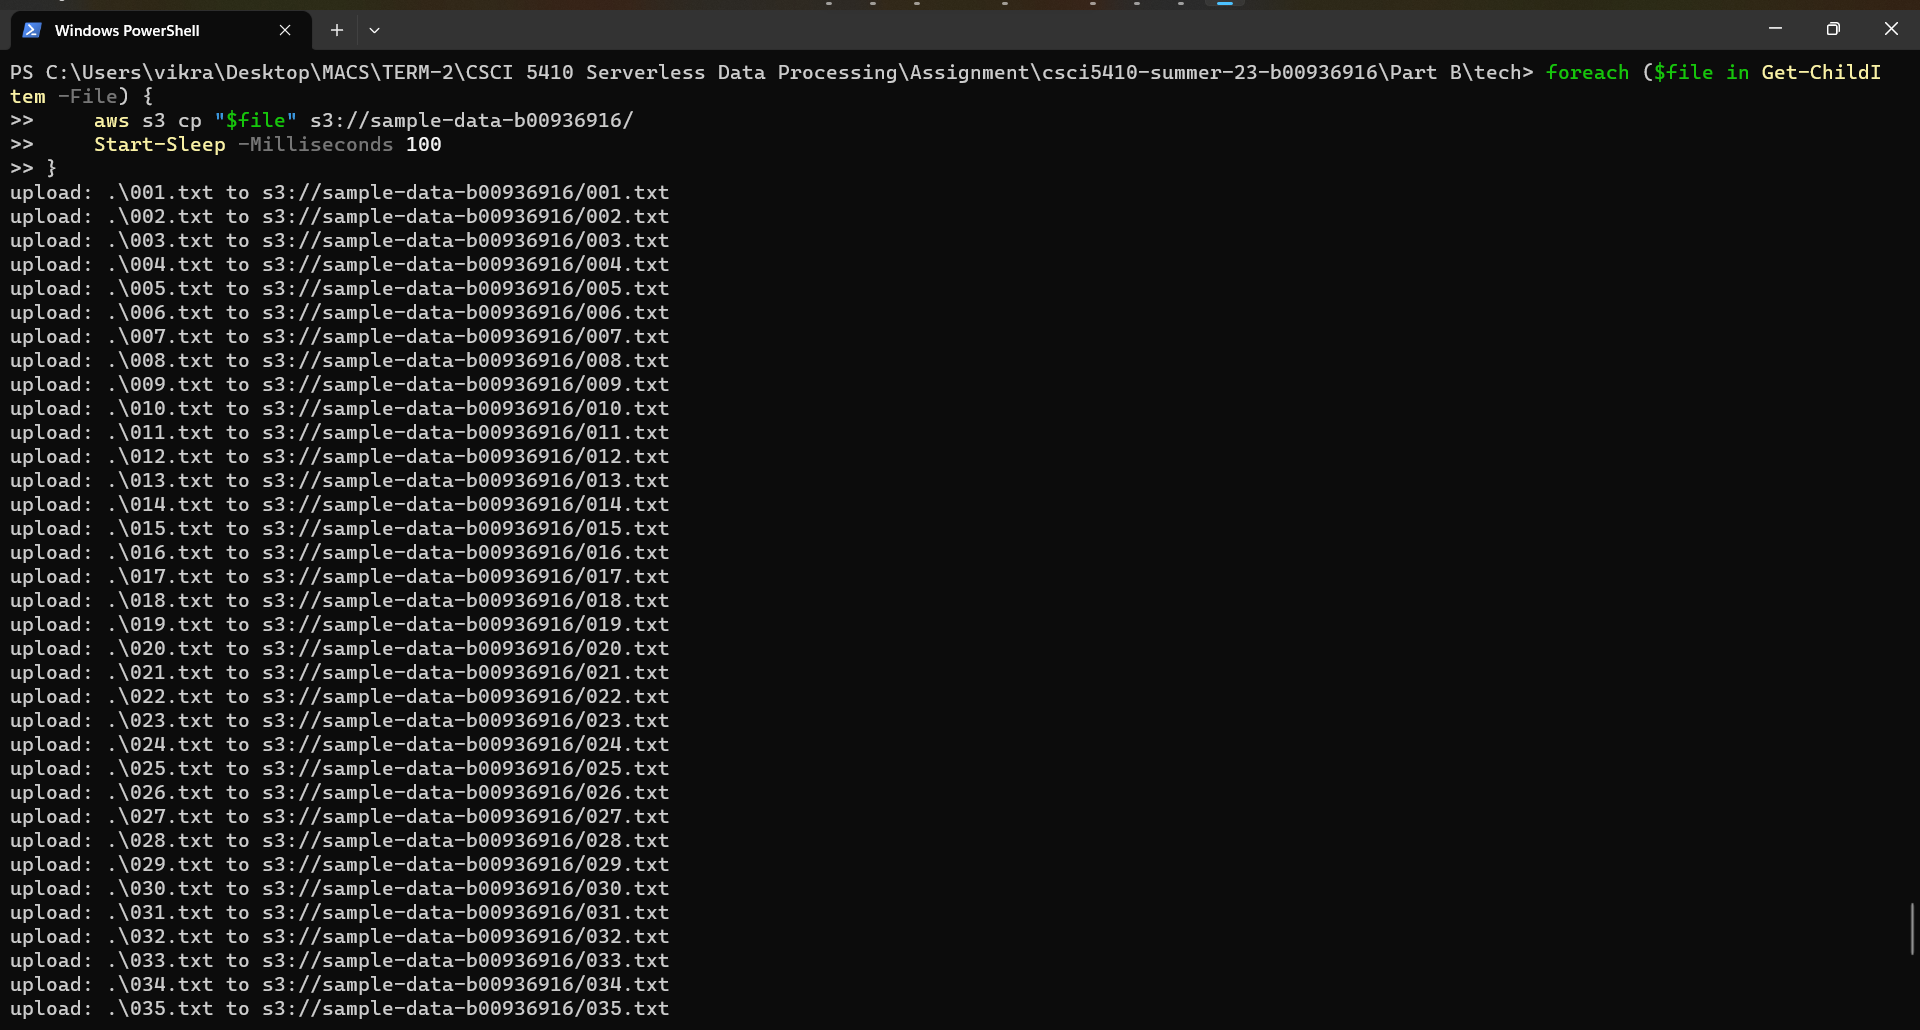
\includegraphics[scale=1, width=15cm,height=7.5cm]{PROBLEM 2/Screenshots/3.1 put object to bucket sample-data-b00936916 in cli.png}}
    \caption{\textbf{\textit{Upload the files in folder 'tech' to bucket sample-data-b00936916 via CLI}}}
    \label{fig:}
\end{figure}


\begin{figure}[htp]
    \centering
    \fbox{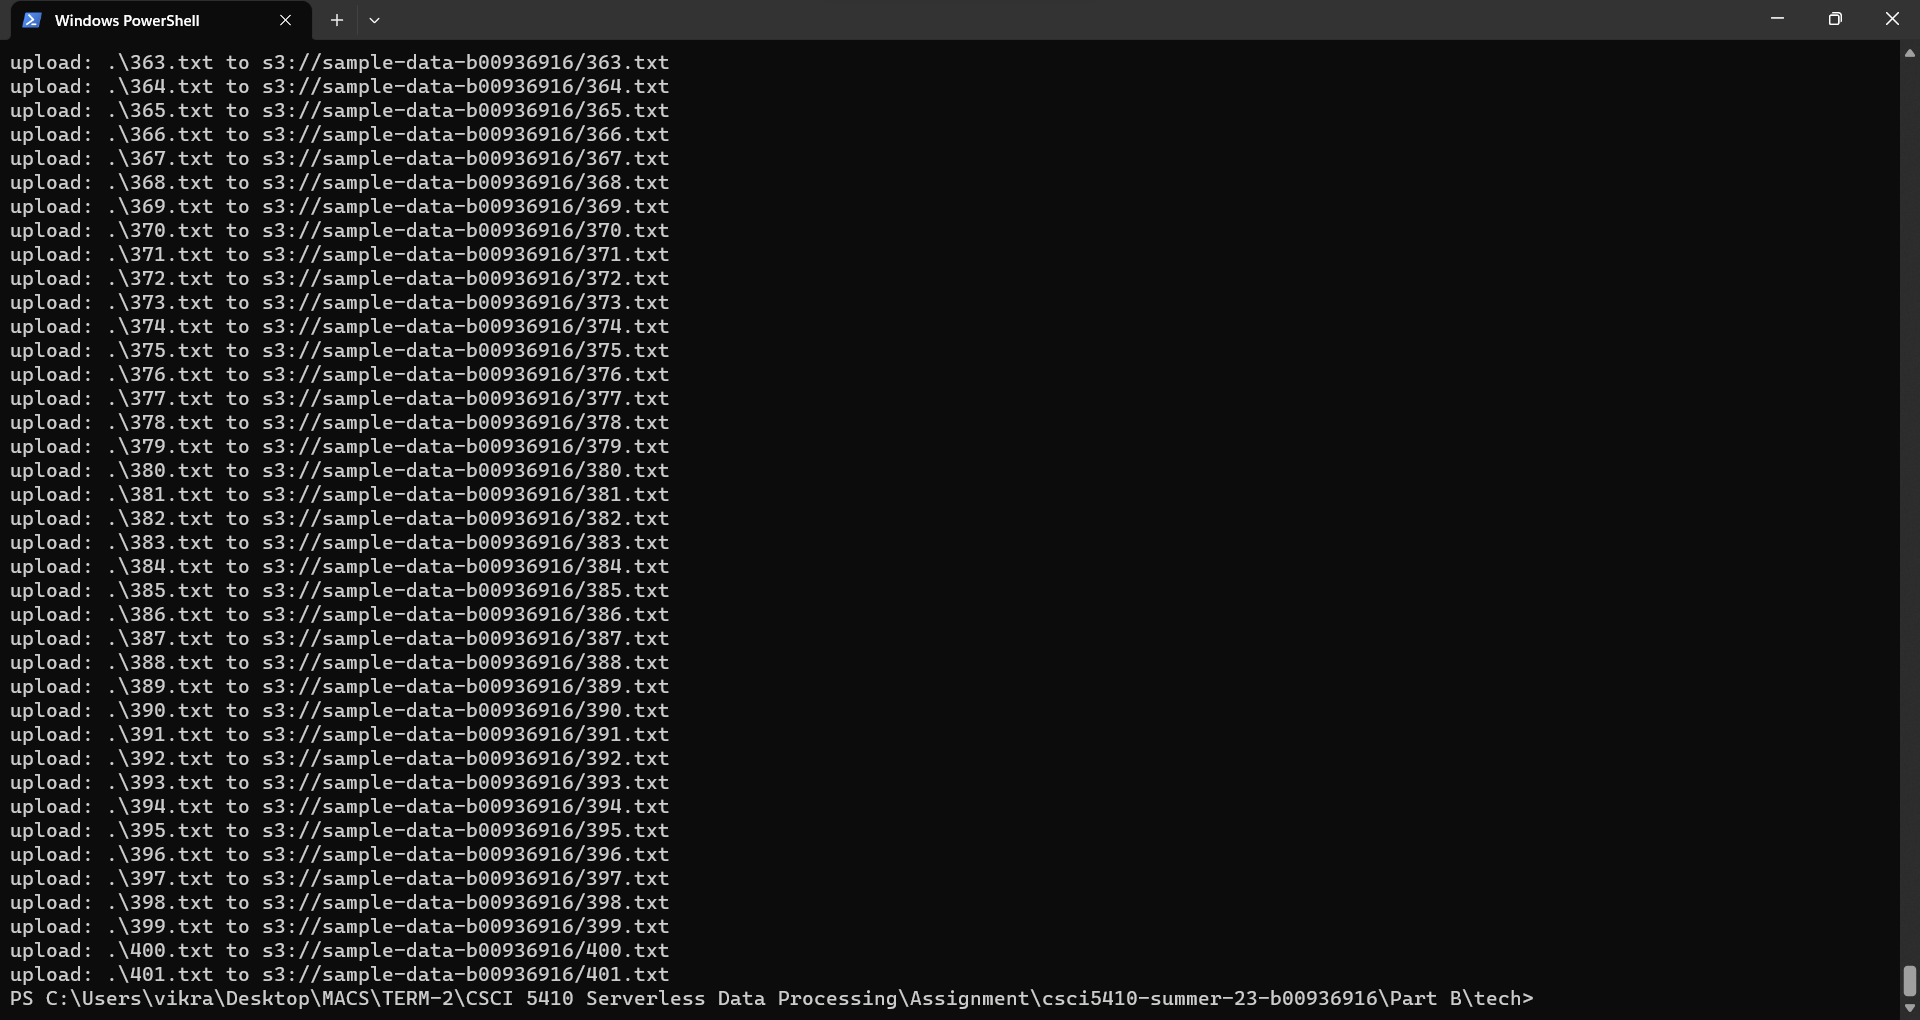
\includegraphics[scale=1, width=15cm,height=7.5cm]{PROBLEM 2/Screenshots/3.2 Testing - put object to 1st bucket via CLI - END 401.png}}
    \caption{\textbf{\textit{Upload the files in folder 'tech' to bucket sample-data-b00936916 via CLI - completed}}}
    \label{fig:}
\end{figure}

\begin{figure}[htp]
    \centering
    \fbox{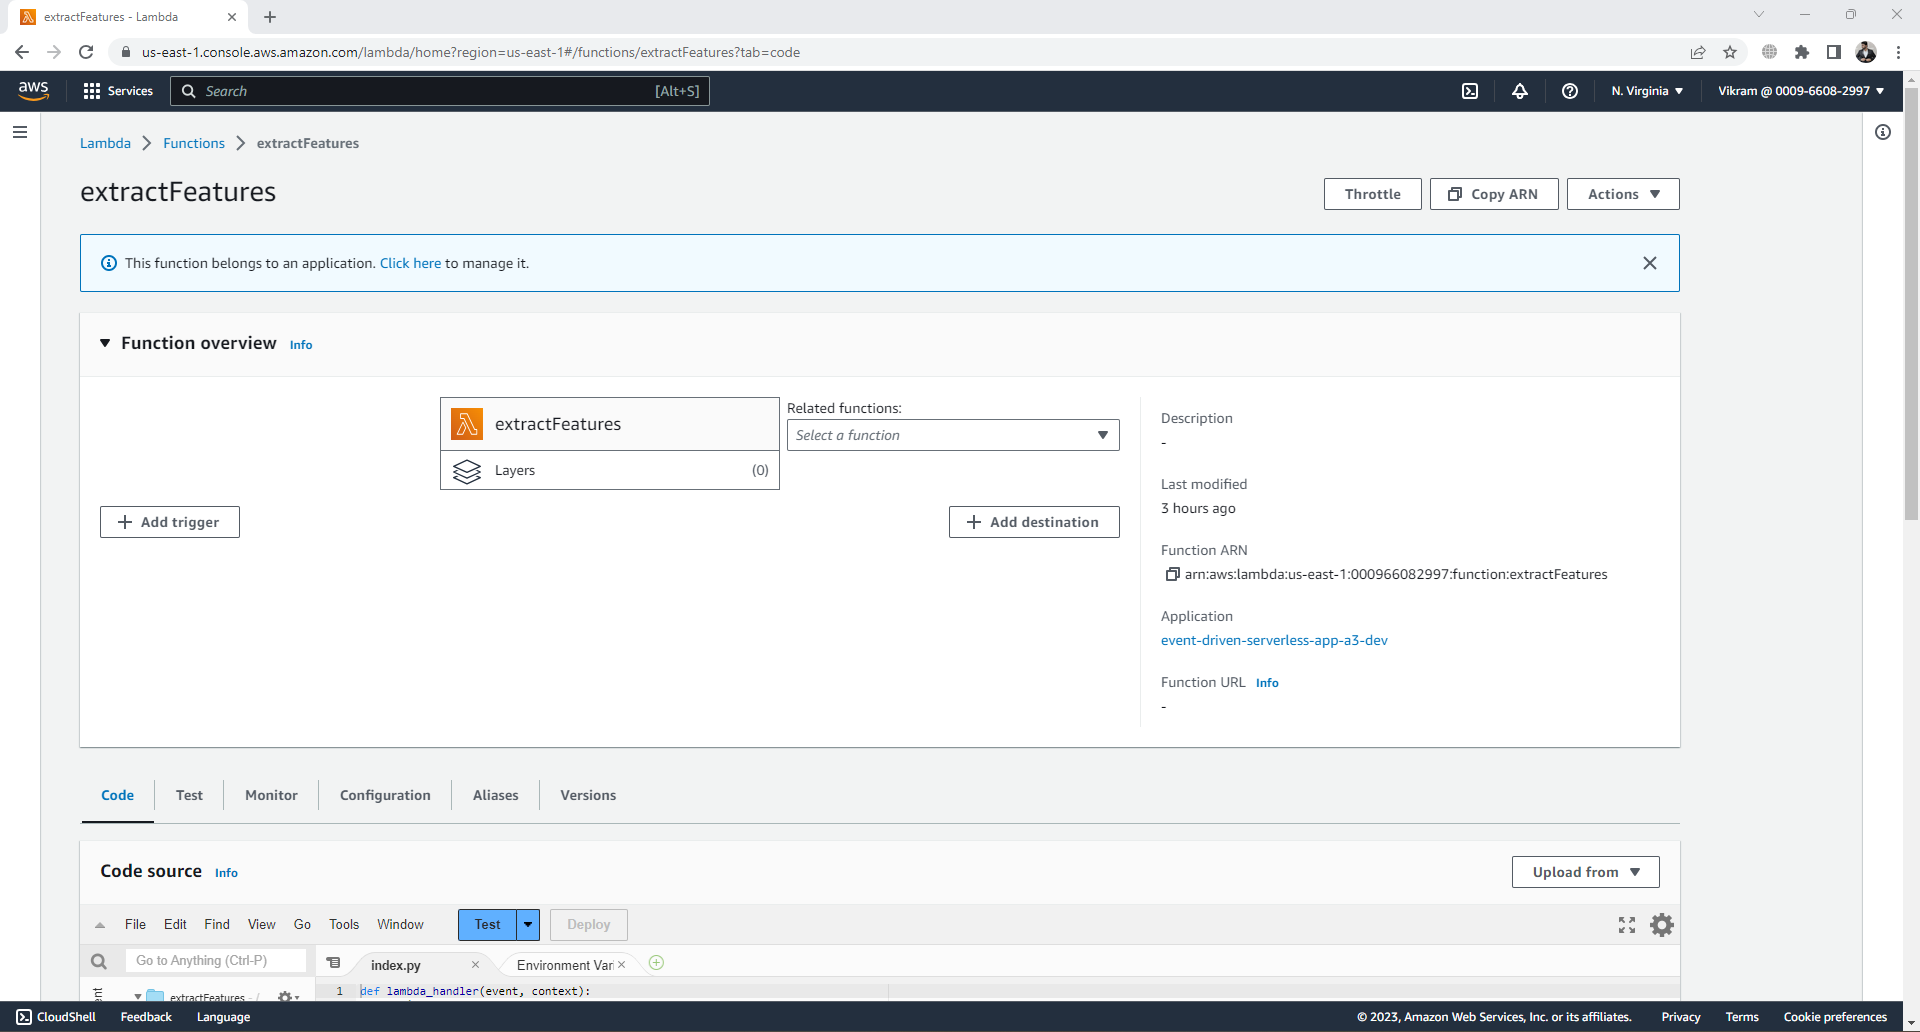
\includegraphics[scale=1, width=15cm,height=7.5cm]{PROBLEM 2/Screenshots/4.0 extractFeatures before adding trigger.png}}
    \caption{\textbf{\textit{extractFeatures lambda before adding trigger}}}
    \label{fig:}
\end{figure}

\begin{figure}[htp]
    \centering
    \fbox{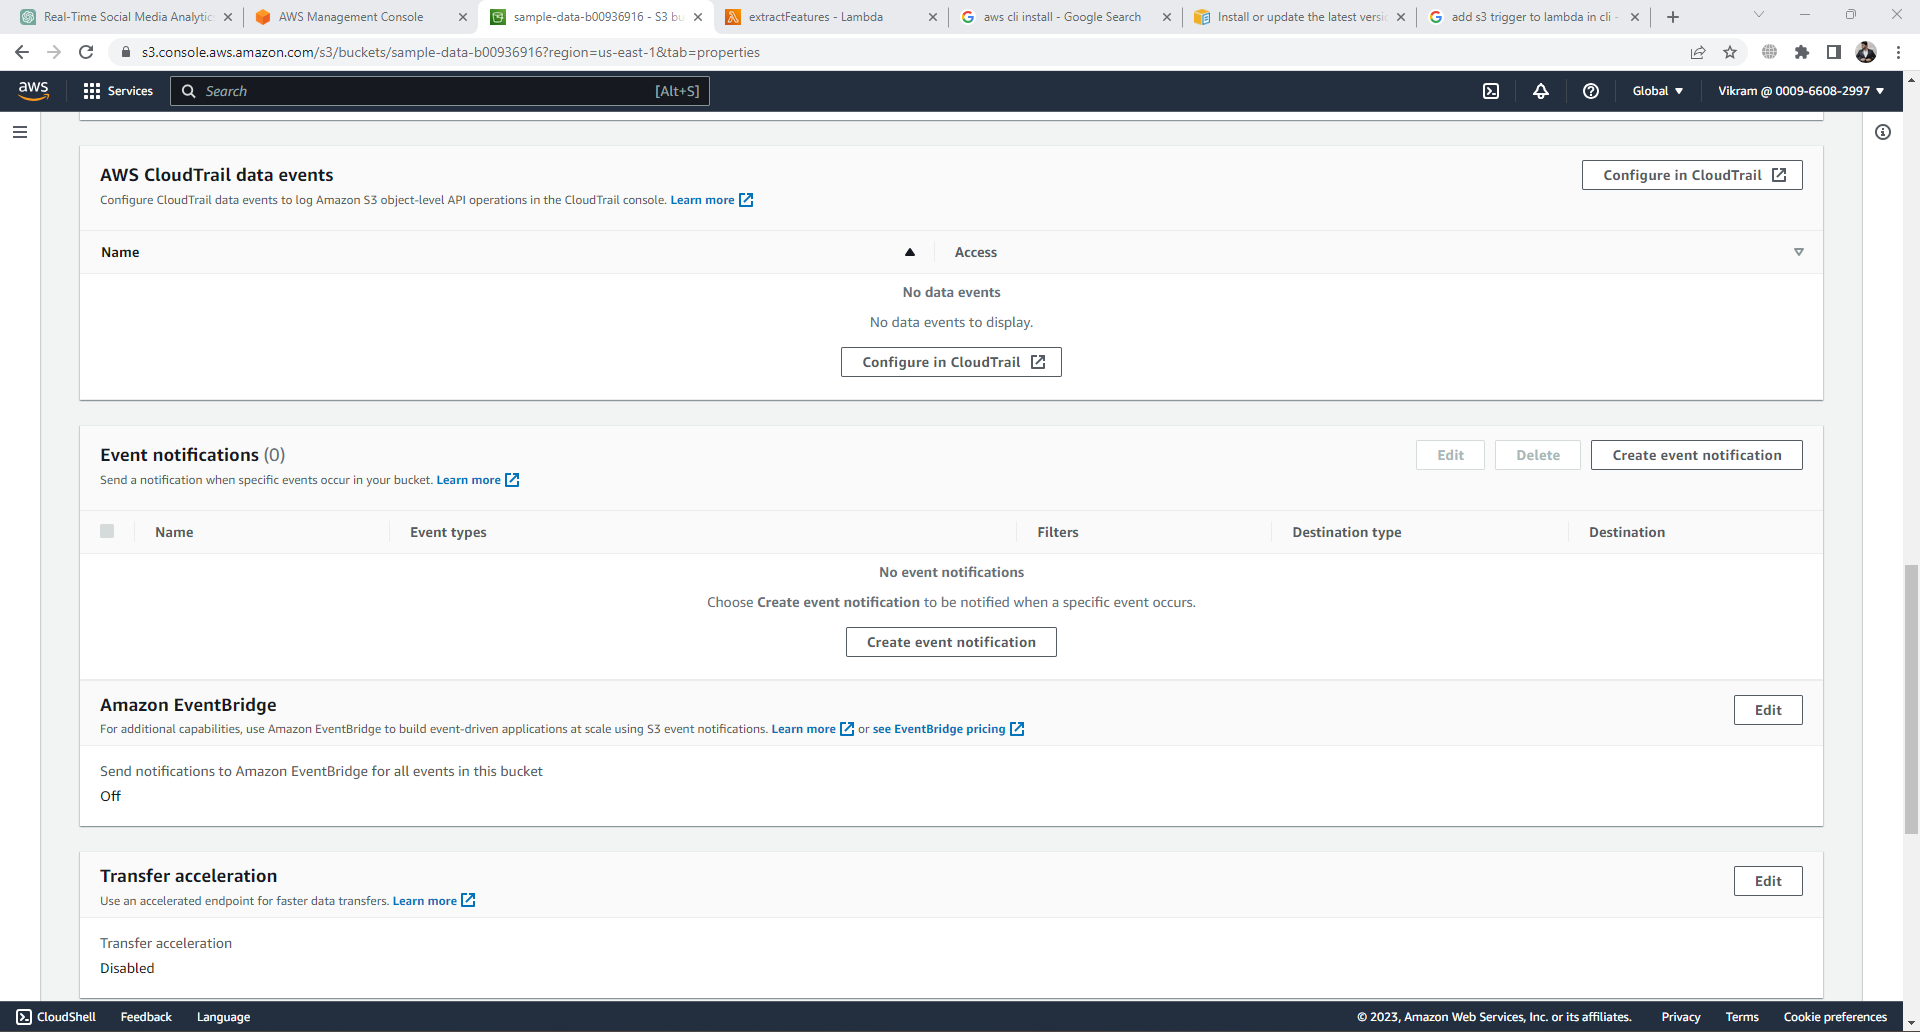
\includegraphics[scale=1, width=15cm,height=7.5cm]{PROBLEM 2/Screenshots/4.1 sample-data-b00936916 before adding event notification.png}}
    \caption{\textbf{\textit{sample-data-b00936916 before adding event notification}}}
    \label{fig:}
\end{figure}

\begin{figure}[htp]
    \centering
    \fbox{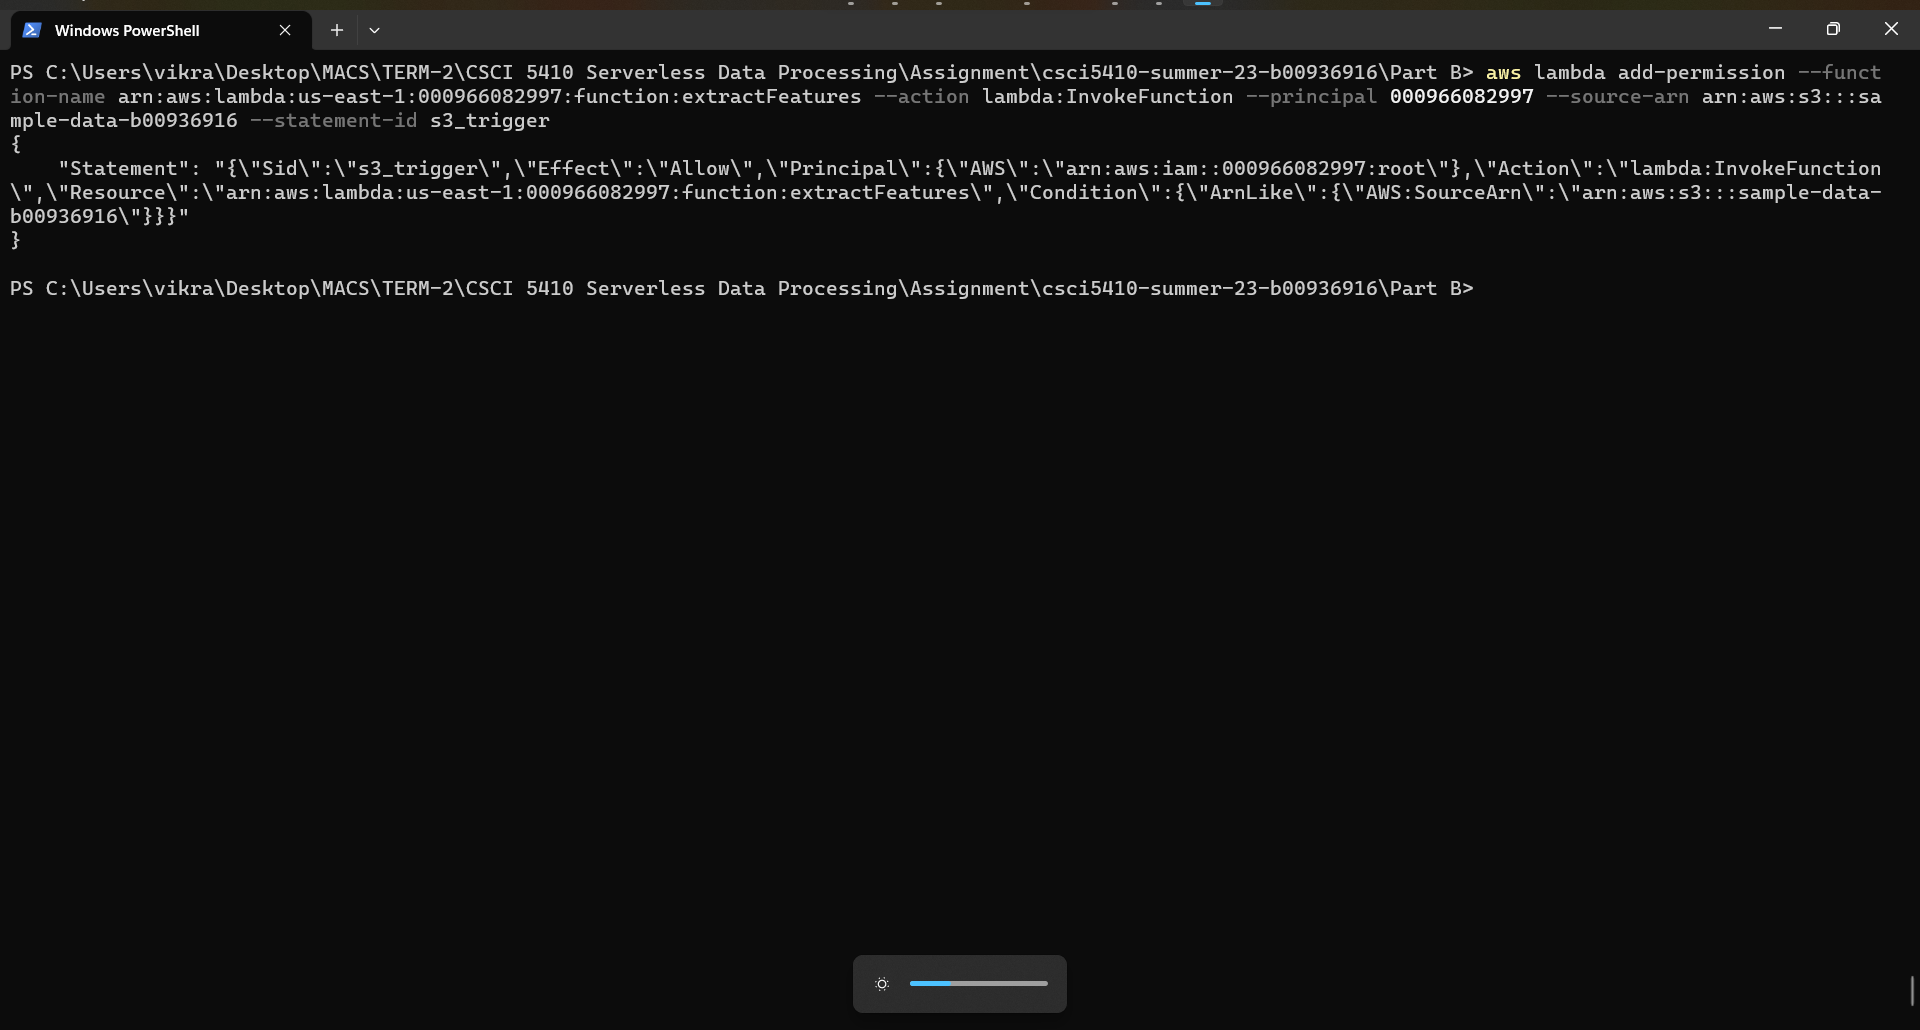
\includegraphics[scale=1, width=15cm,height=7.5cm]{PROBLEM 2/Screenshots/5.1.1 add InvokeFunction permission created in cli.png}}
    \caption{\textbf{\textit{add InvokeFunction permission for lambda sample-data-b00936916 via CLI}}}
    \label{fig:}
\end{figure}

\begin{figure}[htp]
    \centering
    \fbox{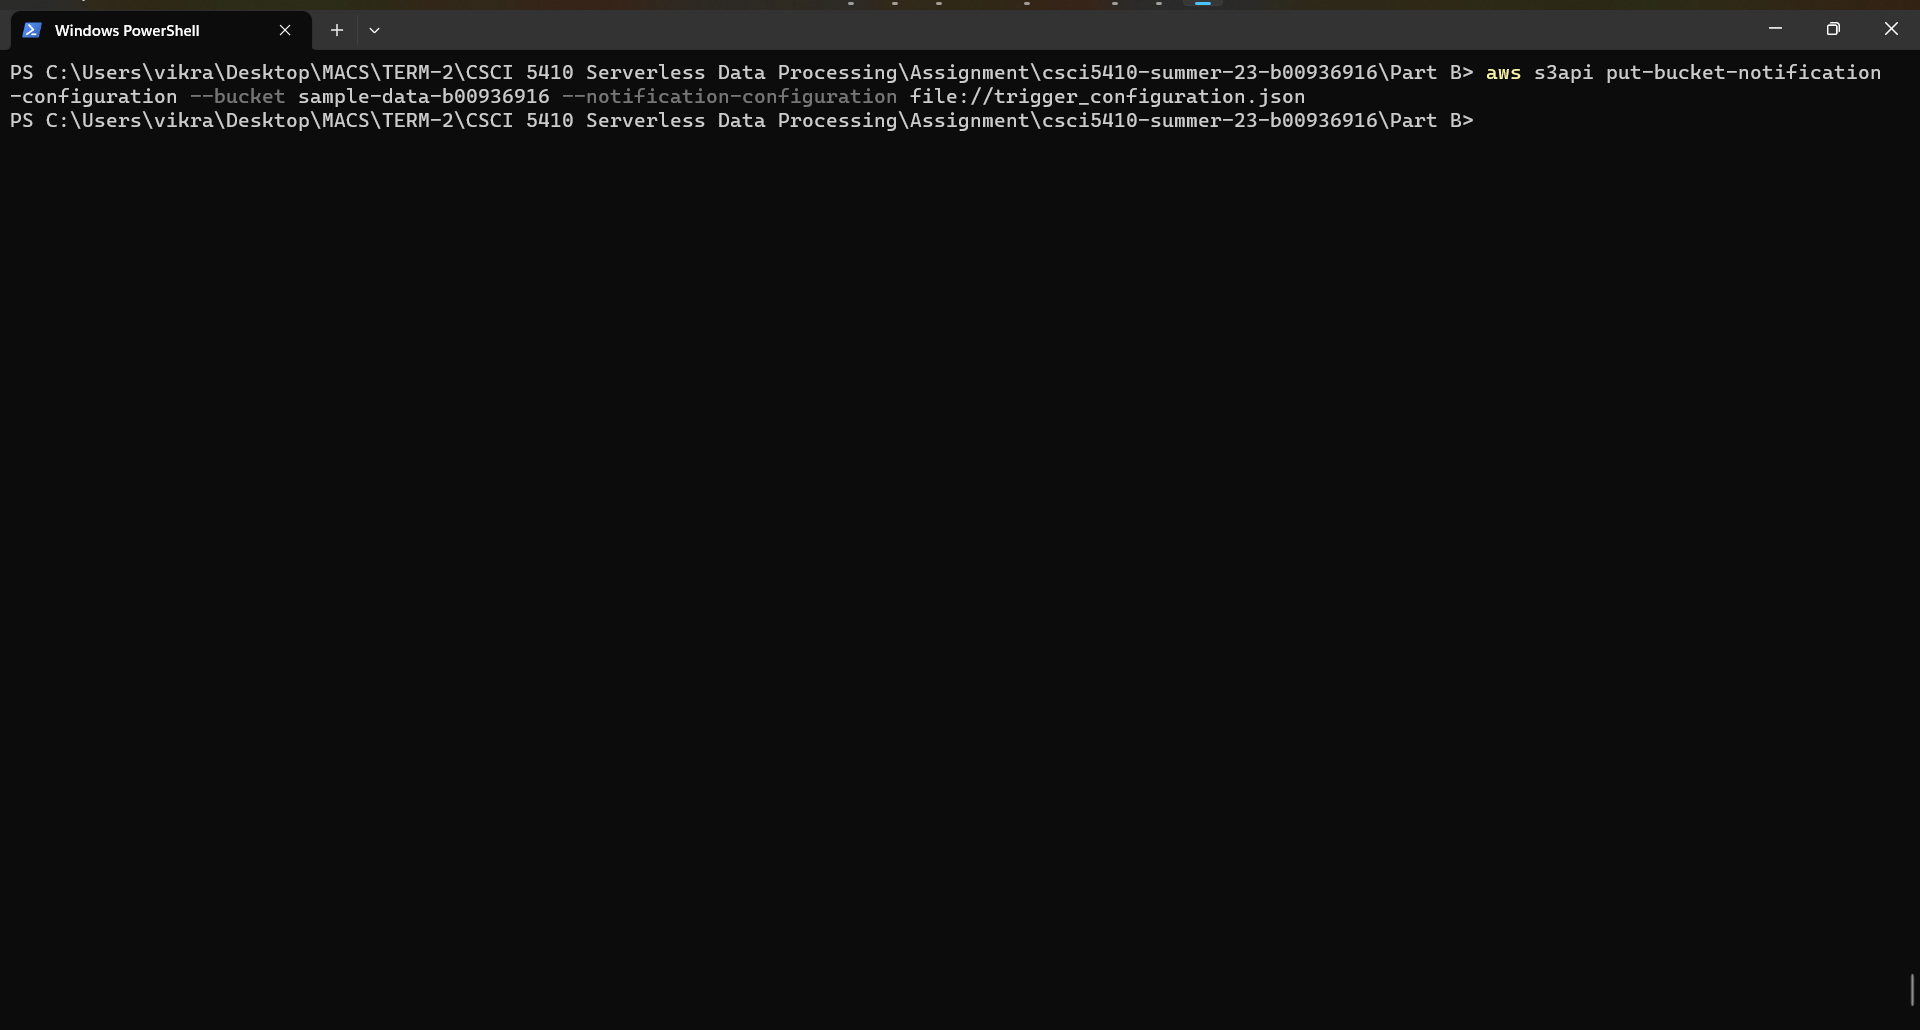
\includegraphics[scale=1, width=15cm,height=7.5cm]{PROBLEM 2/Screenshots/5.2 add s3 trigger via cli for extractFeatures lambda.png}}
    \caption{\textbf{\textit{Add s3 trigger via CLI for extractFeatures lambda}}}
    \label{fig:}
\end{figure}

\begin{figure}[htp]
    \centering
    \fbox{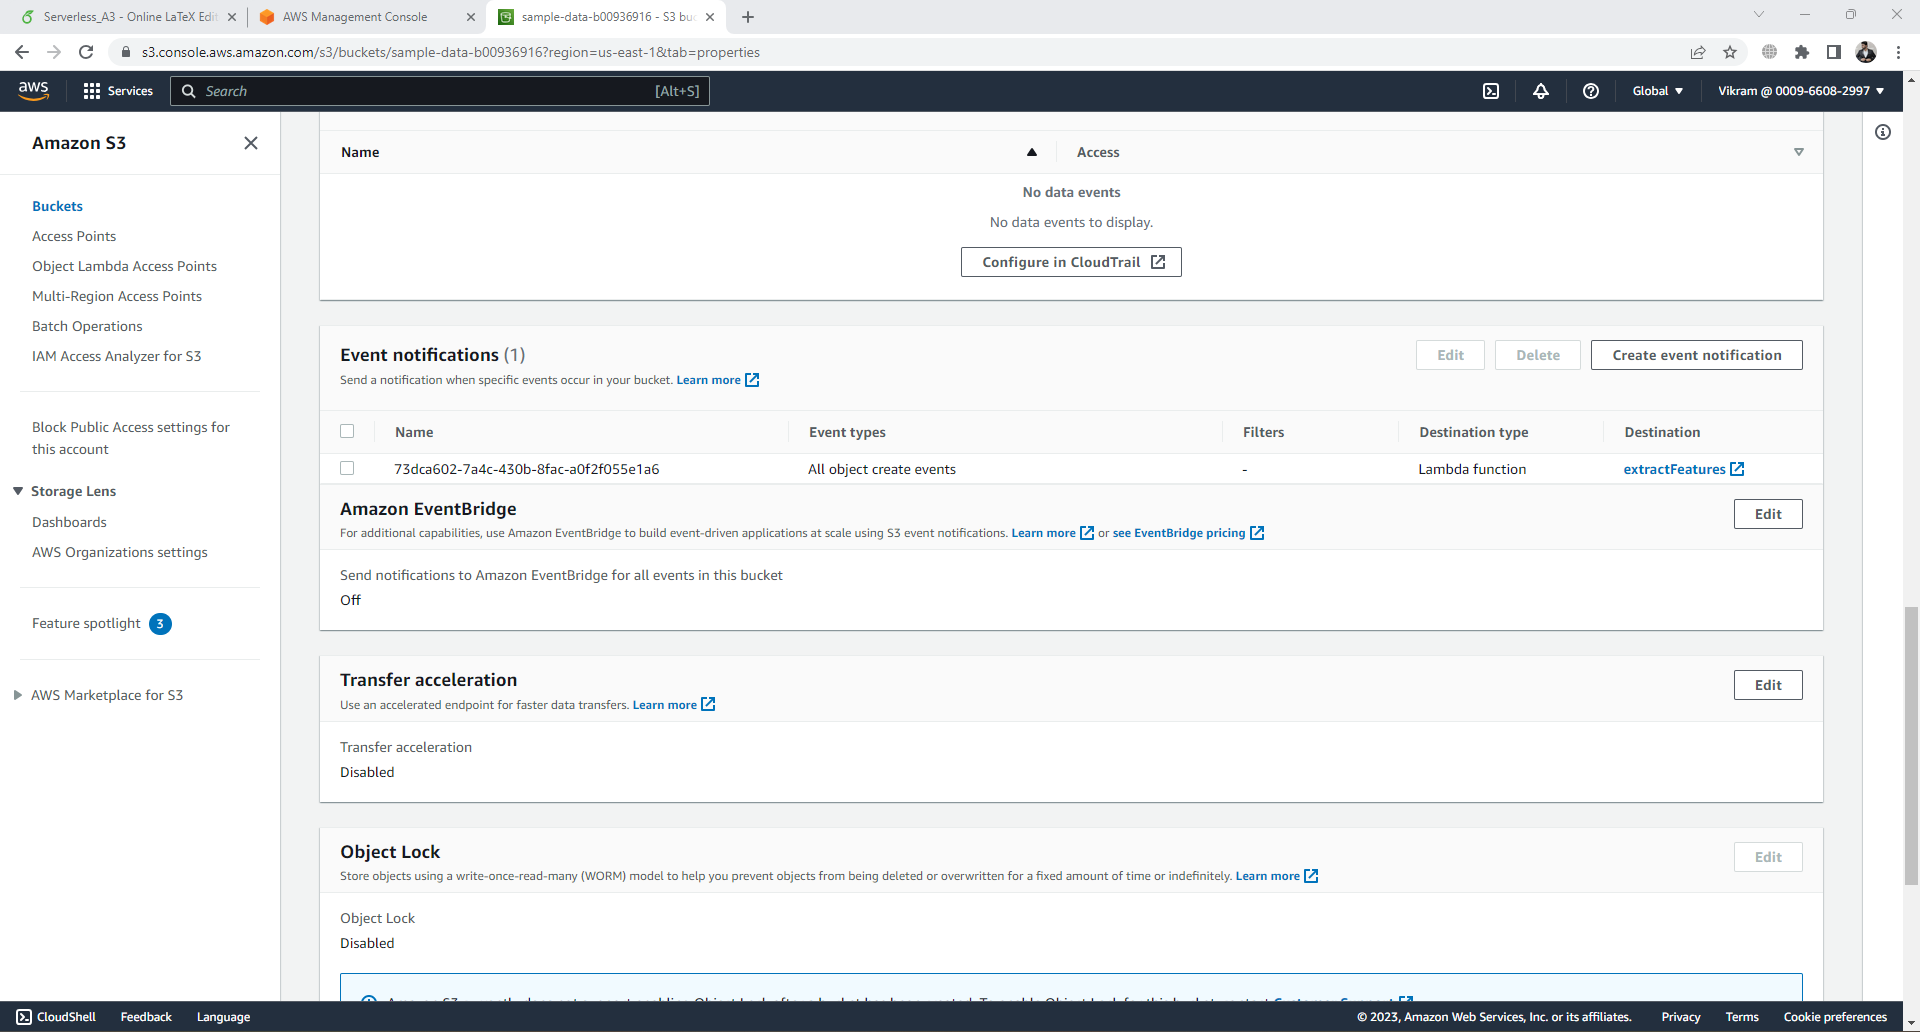
\includegraphics[scale=1, width=15cm,height=7.5cm]{PROBLEM 2/Screenshots/5.3.1 s3 event notification - bucket sample-data-b00936916.png}}
    \caption{\textbf{\textit{S3 event notification - bucket sample-data-b00936916}}}
    \label{fig:}
\end{figure}


\begin{figure}[htp]
    \centering
    \fbox{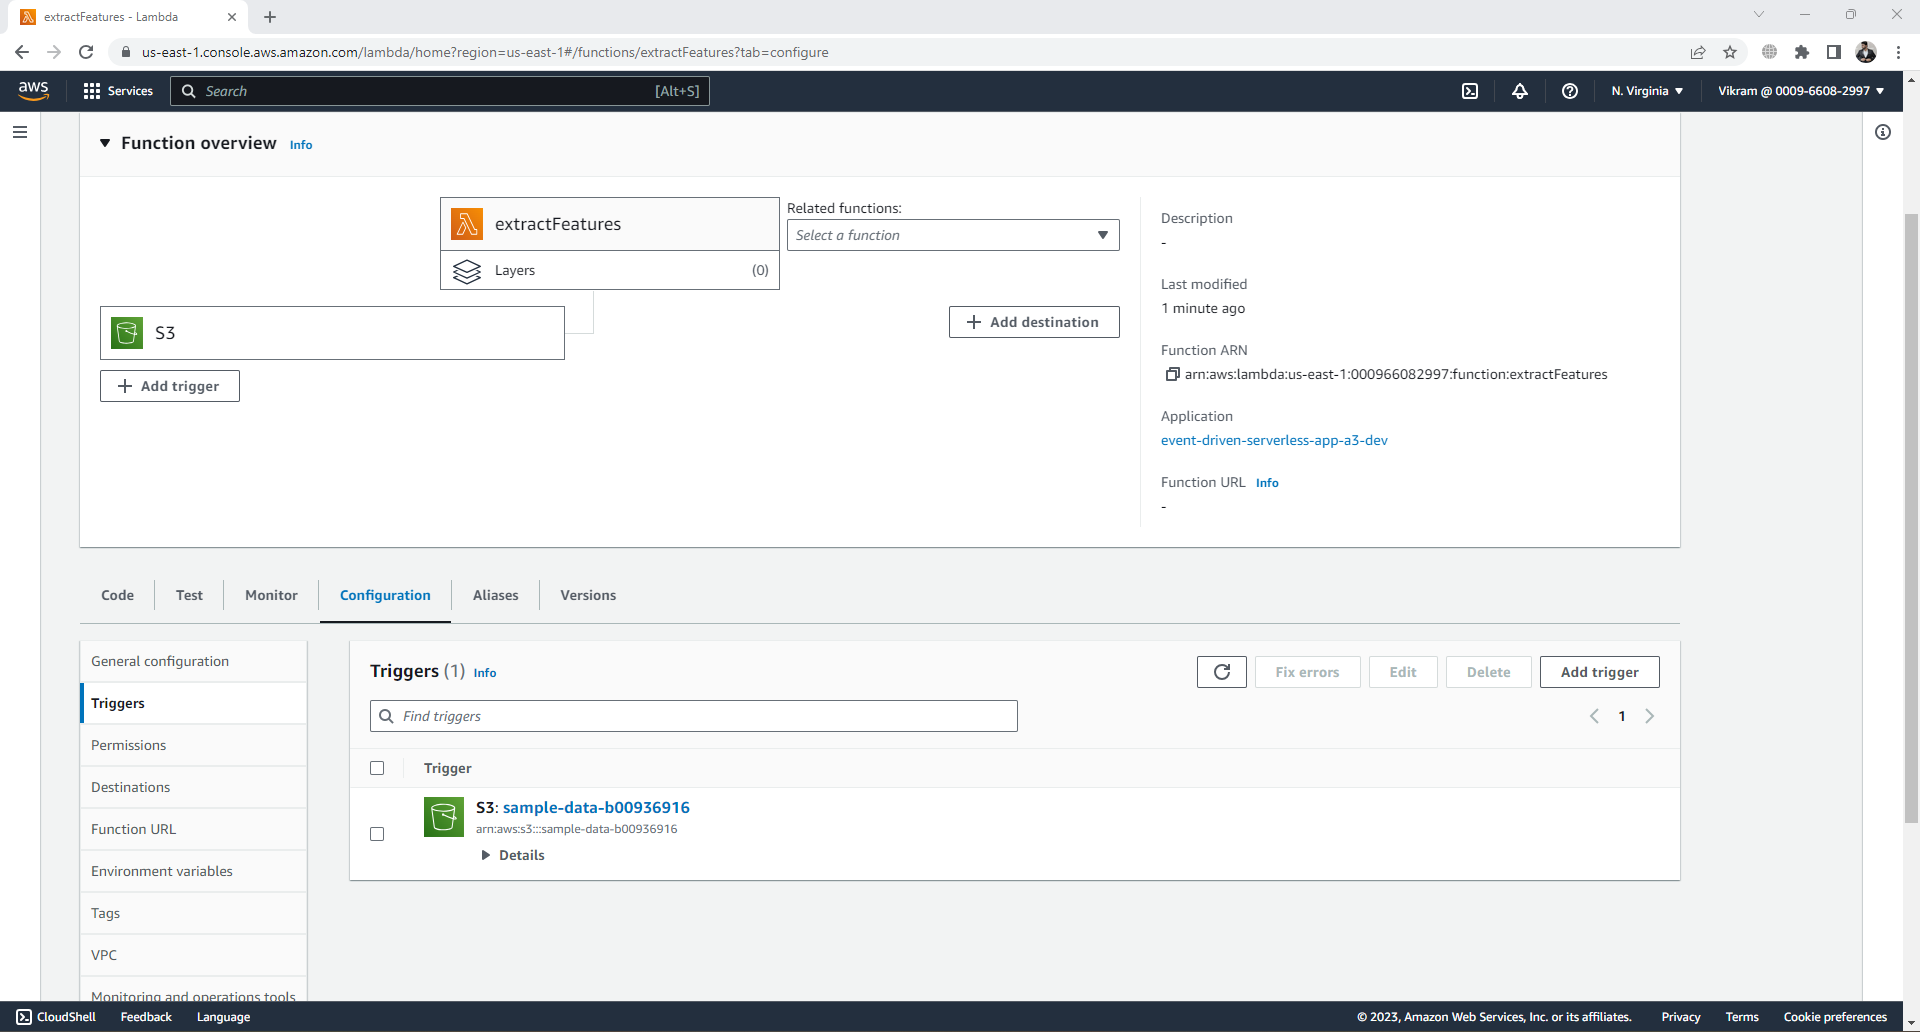
\includegraphics[scale=1, width=15cm,height=7.5cm]{PROBLEM 2/Screenshots/5.3 s3 trigger added.png}}
    \caption{\textbf{\textit{S3 trigger added for lambda extractFeatures}}}
    \label{fig:}
\end{figure}

\begin{figure}[htp]
    \centering
    \fbox{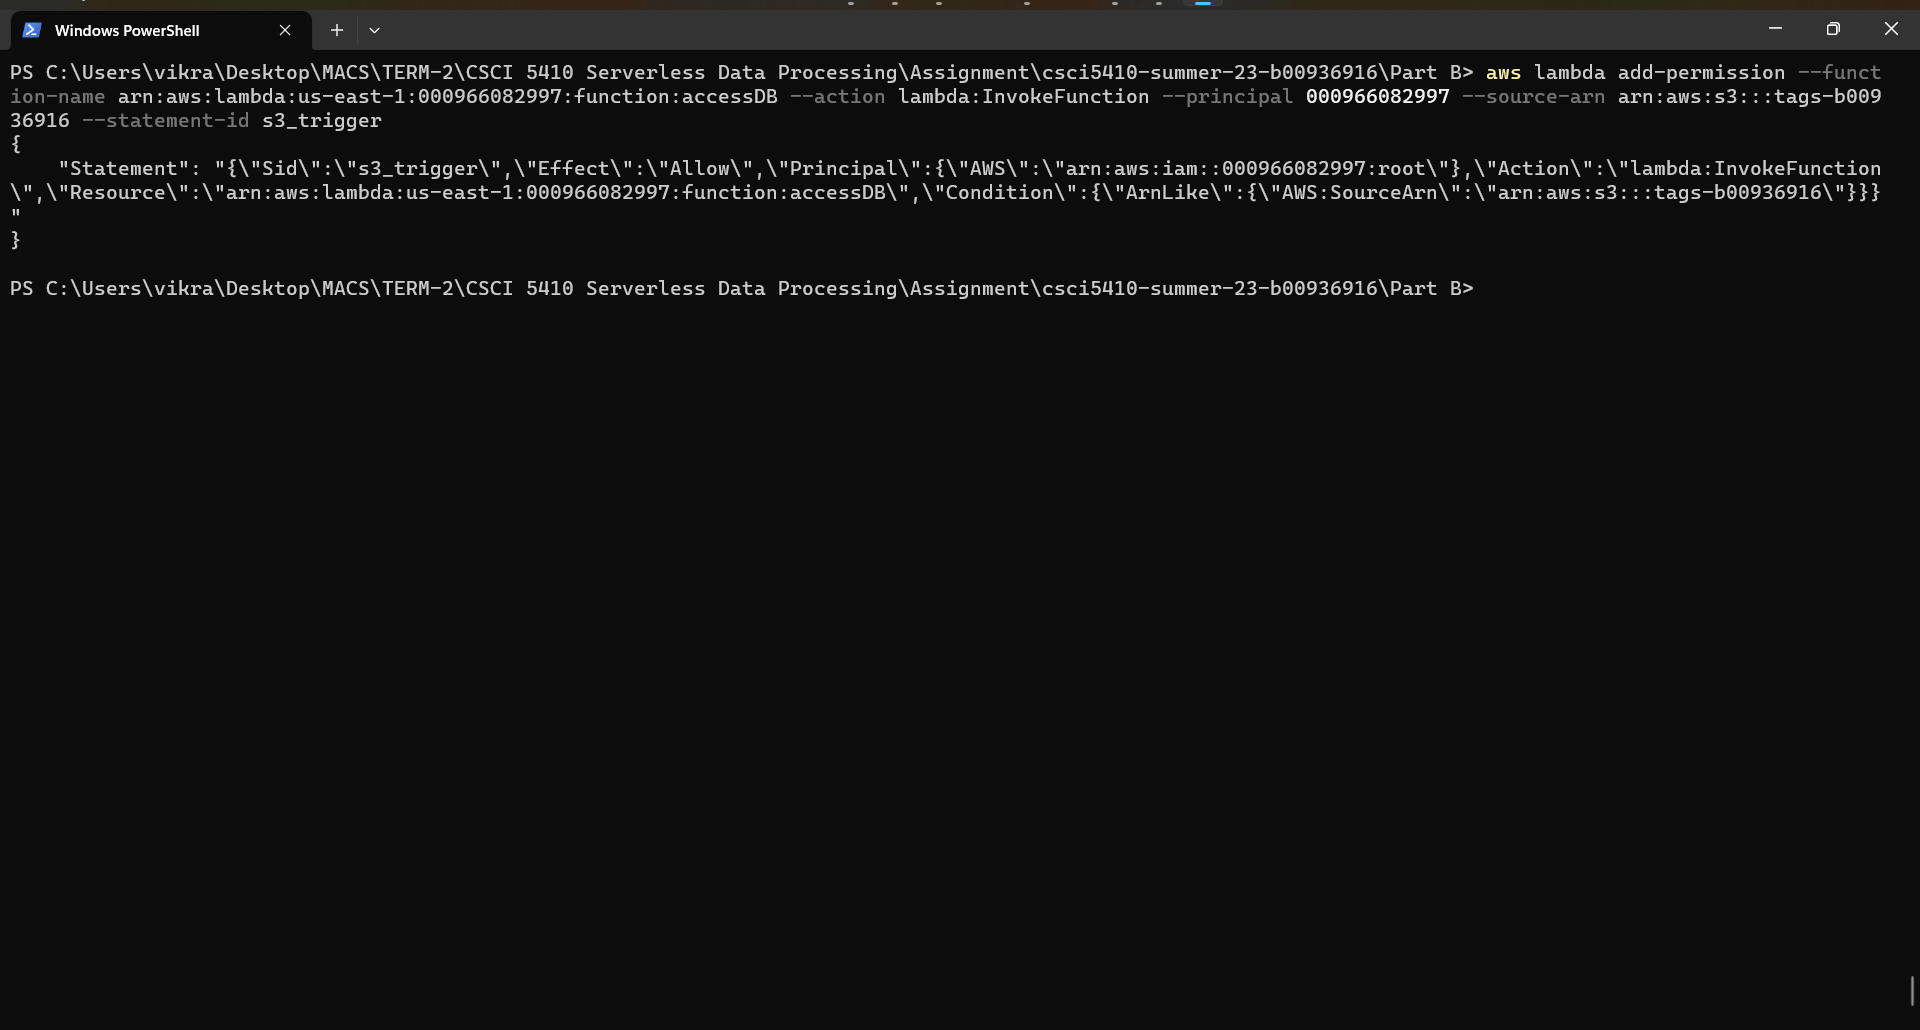
\includegraphics[scale=1, width=15cm,height=7.5cm]{PROBLEM 2/Screenshots/6.1 add InvokeFunction permission for tags-b00936916 bucket created in cli.png}}
    \caption{\textbf{\textit{add InvokeFunction permission for lambda tags-b00936916 via CLI}}}
    \label{fig:}
\end{figure}

\begin{figure}[htp]
    \centering
    \fbox{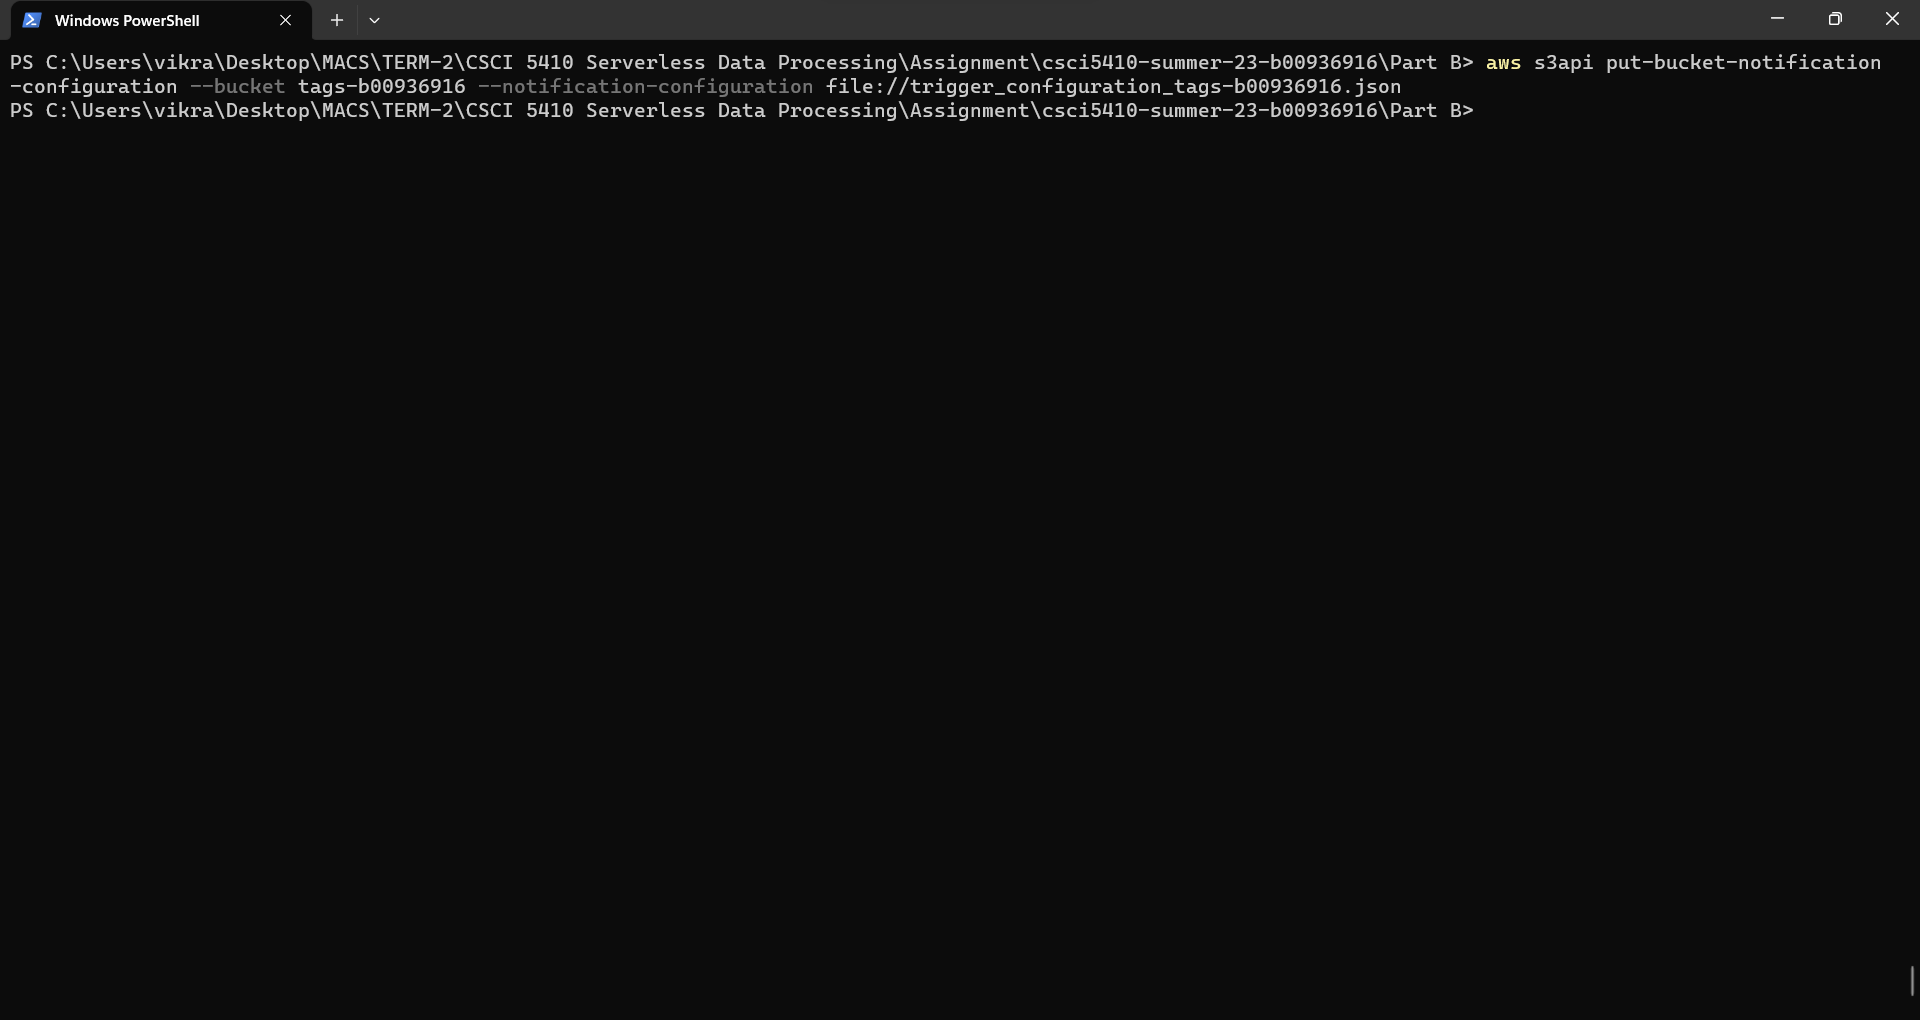
\includegraphics[scale=1, width=15cm,height=7.5cm]{PROBLEM 2/Screenshots/6.2 add s3 trigger via cli for accessDB lambda.png}}
    \caption{\textbf{\textit{Add s3 trigger via CLI for accessDB lambda}}}
    \label{fig:}
\end{figure}

\begin{figure}[htp]
    \centering
    \fbox{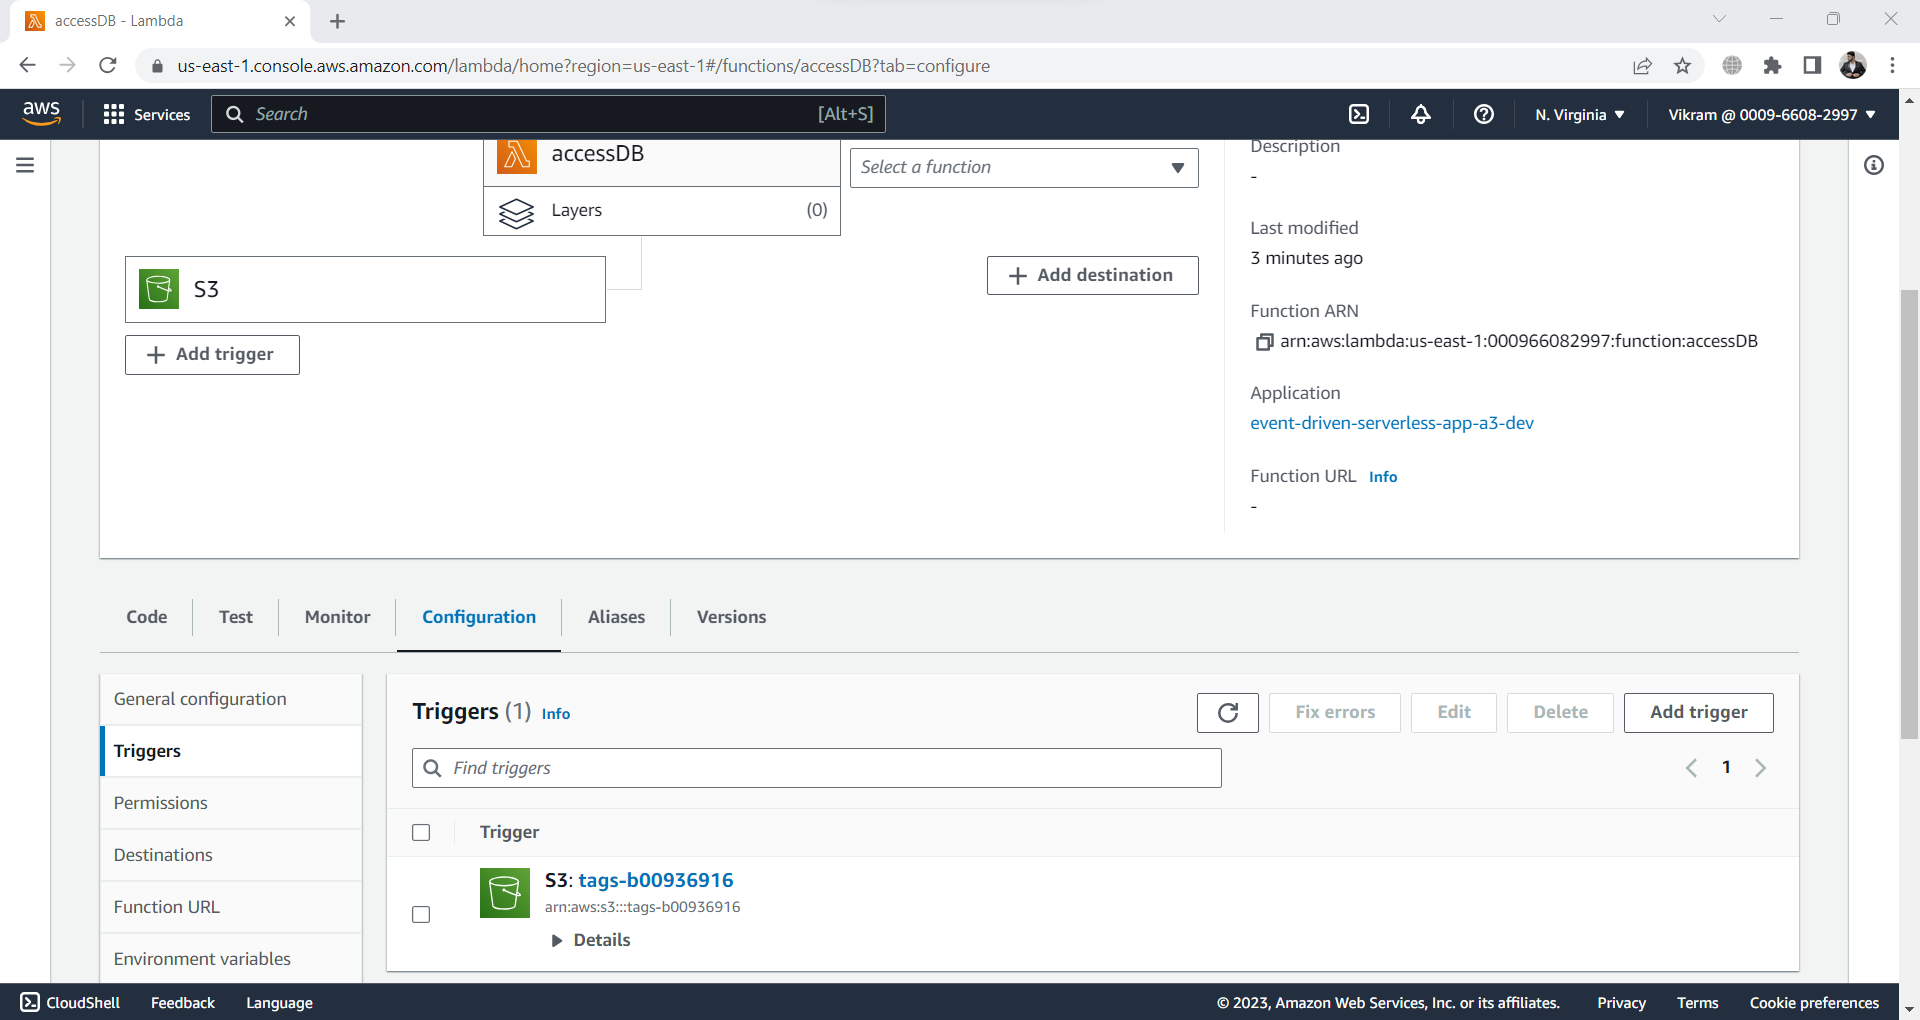
\includegraphics[scale=1, width=15cm,height=7.5cm]{PROBLEM 2/Screenshots/6.3 s3 trigger added.png}}
    \caption{\textbf{\textit{S3 trigger added for lambda accessDB}}}
    \label{fig:}
\end{figure}

\begin{figure}[htp]
    \centering
    \fbox{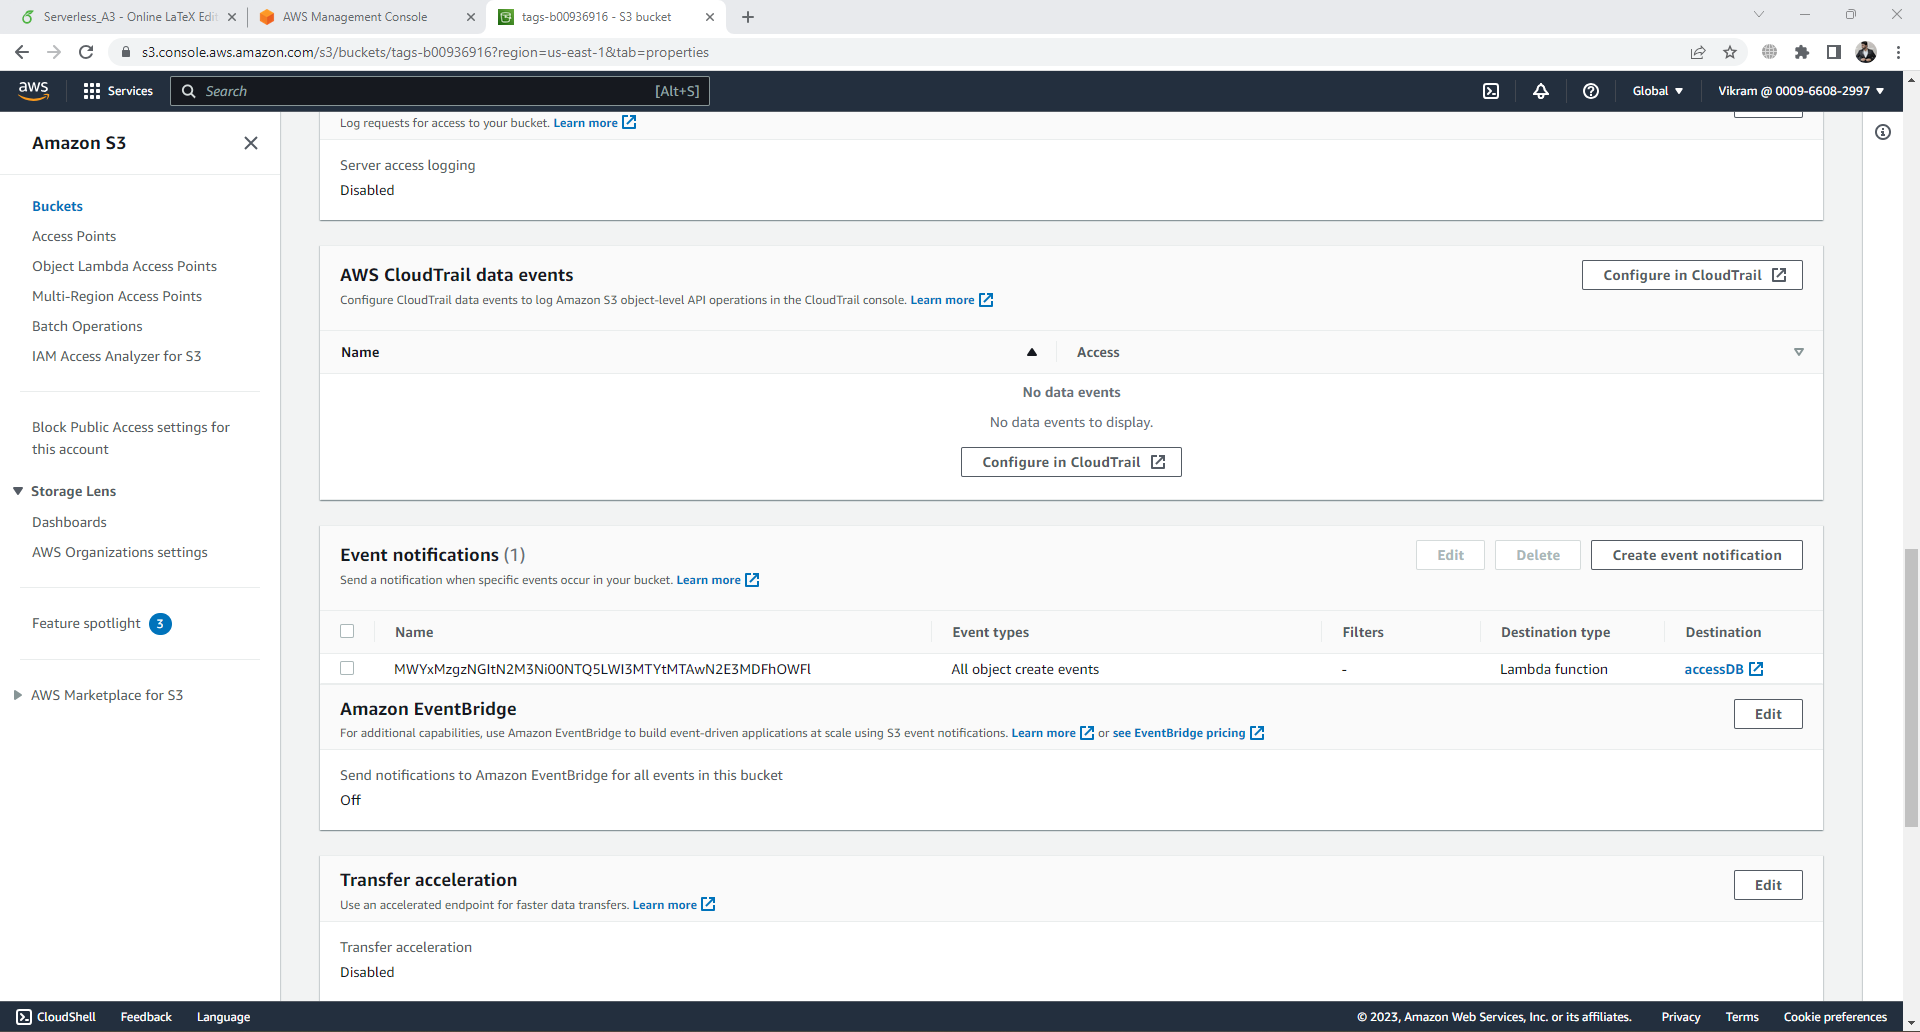
\includegraphics[scale=1, width=15cm,height=7.5cm]{PROBLEM 2/Screenshots/6.2.1 s3 event notififcation for bucket tags-b00936916.png}}
    \caption{\textbf{\textit{S3 event notification for bucket tags-b00936916}}}
    \label{fig:}
\end{figure}

\begin{figure}[htp]
    \centering
    \fbox{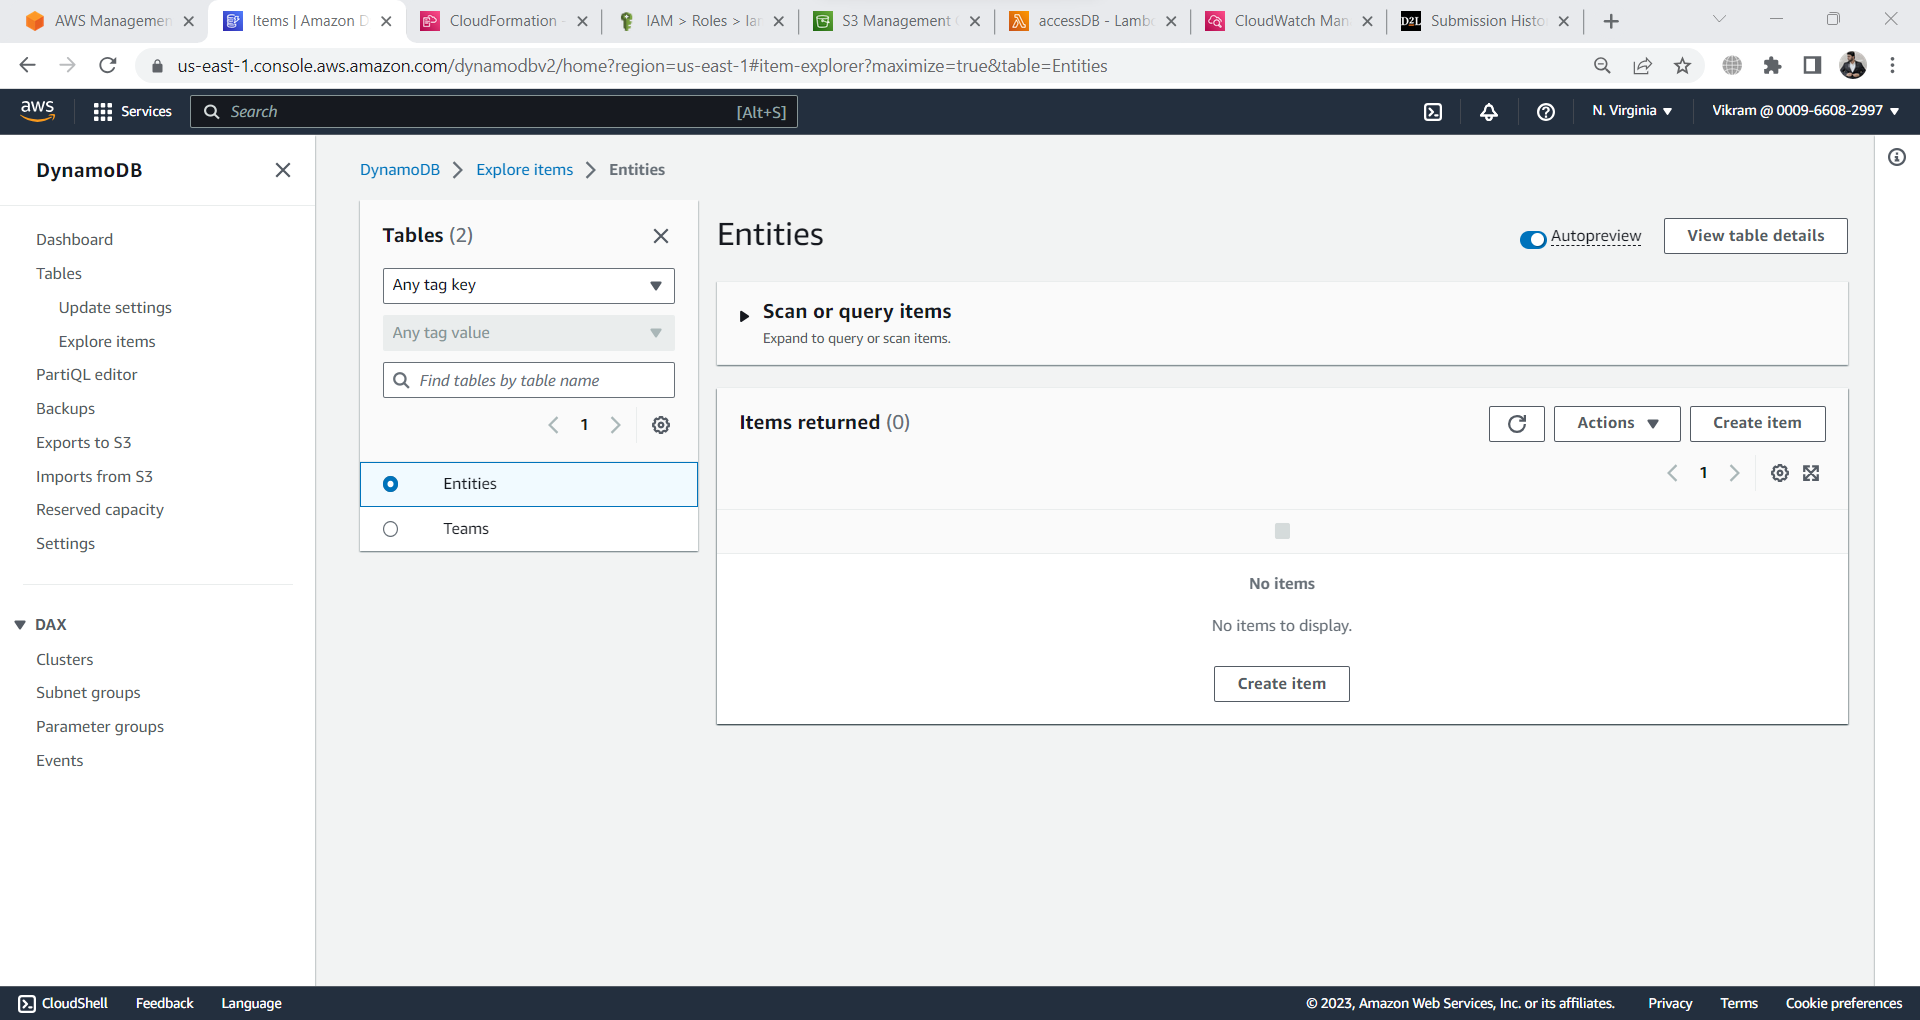
\includegraphics[scale=1, width=15cm,height=7.5cm]{PROBLEM 2/Screenshots/7.1 empty table Entities.png}}
    \caption{\textbf{\textit{Empty DynamoDB table 'Entities'}}}
    \label{fig:}
\end{figure}

\begin{figure}[htp]
    \centering
    \fbox{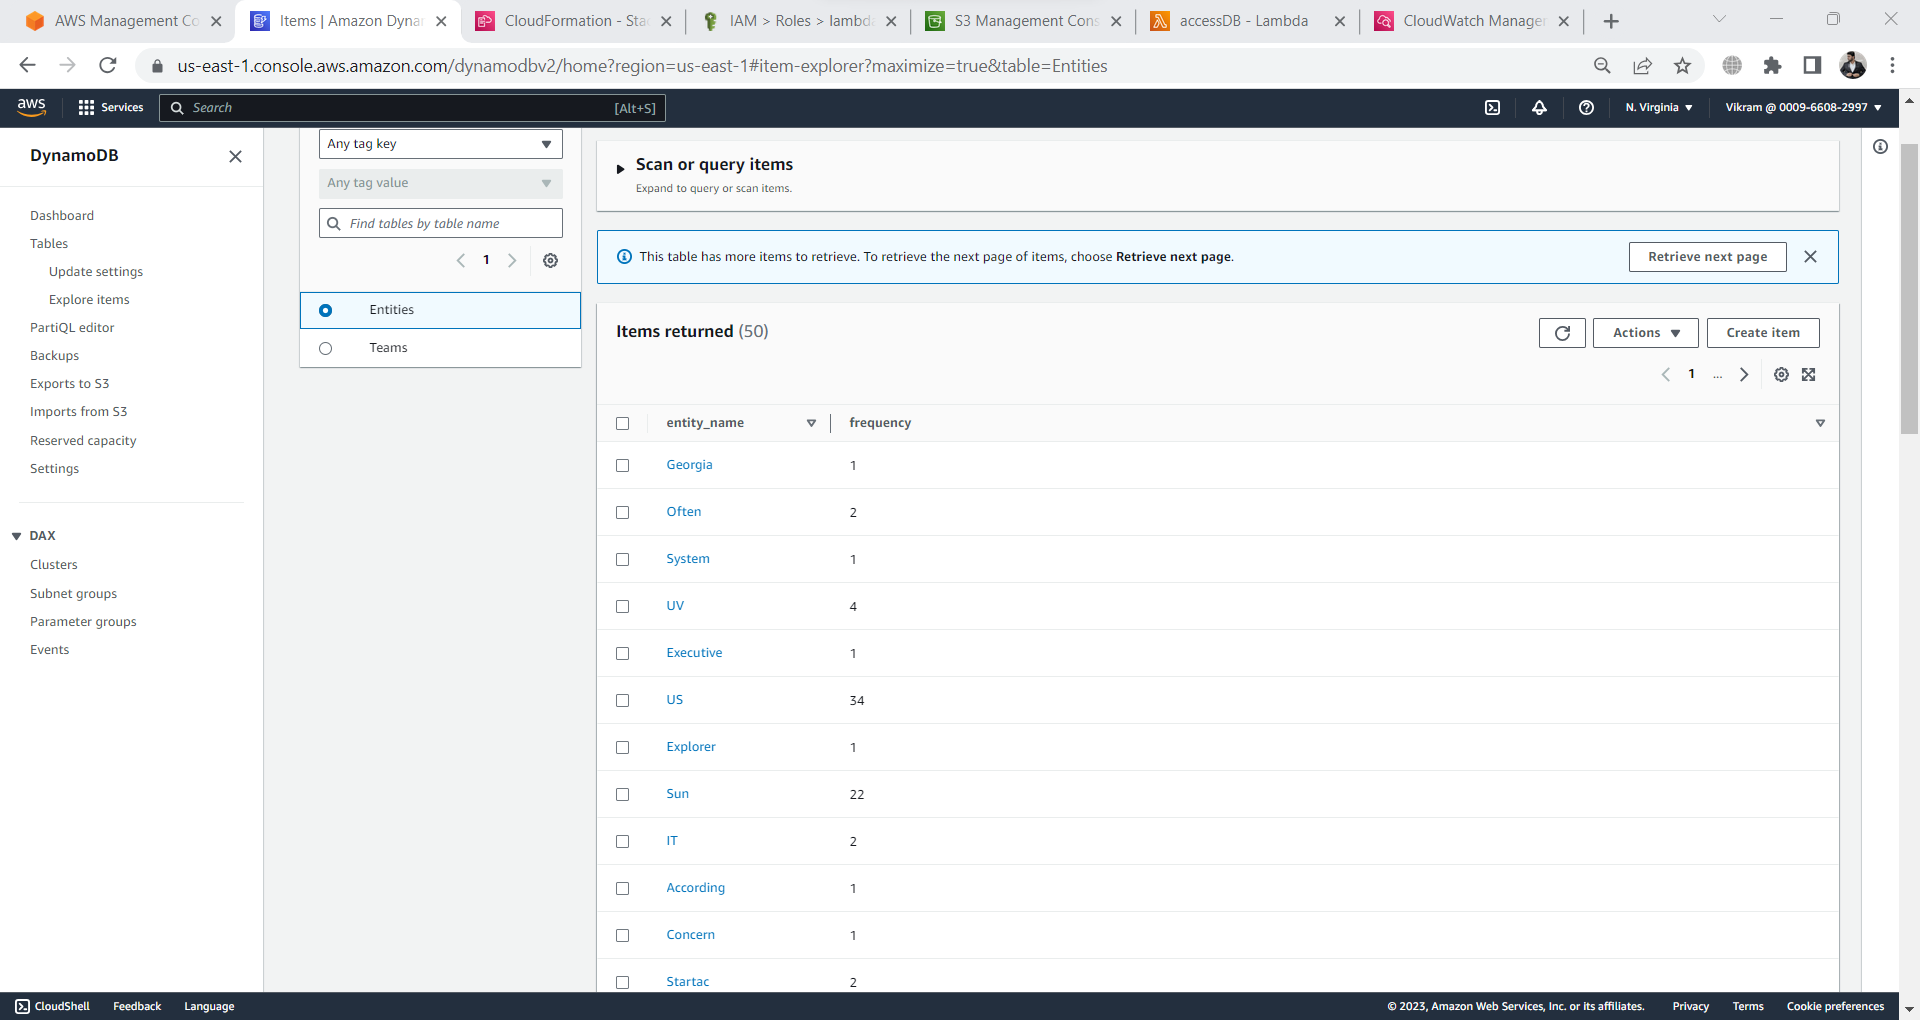
\includegraphics[scale=1, width=15cm,height=7.5cm]{PROBLEM 2/Screenshots/7.2 table after lambda trigger.png}}
    \caption{\textbf{\textit{Final DynamoDB table 'Entities' after all entities are extracted}}}
    \label{fig:}
\end{figure}

\begin{figure}[htp]
    \centering
    \fbox{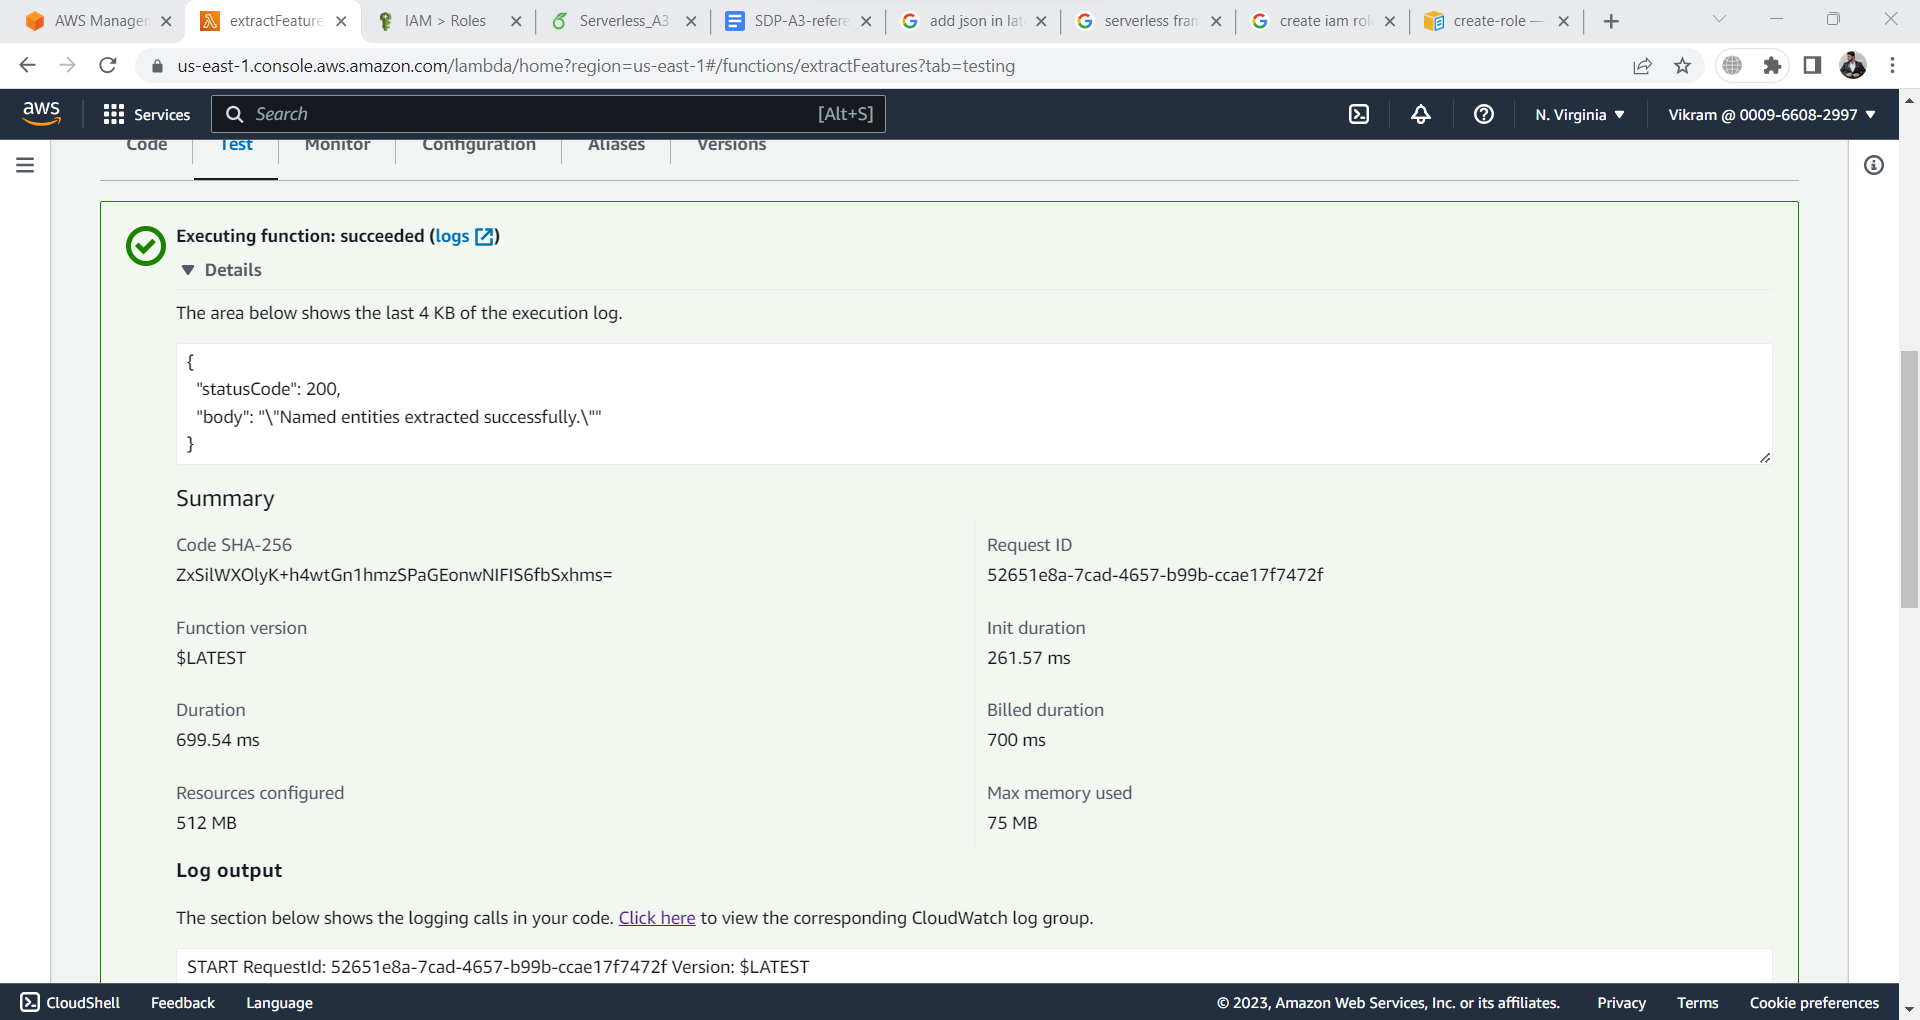
\includegraphics[scale=1, width=15cm,height=7.5cm]{PROBLEM 2/Screenshots/8.1 extractFeatures unit test.png}}
    \caption{\textbf{\textit{ extractFeatures lambda unit test}}}
    \label{fig:}
\end{figure}


\begin{figure}[htp]
    \centering
    \fbox{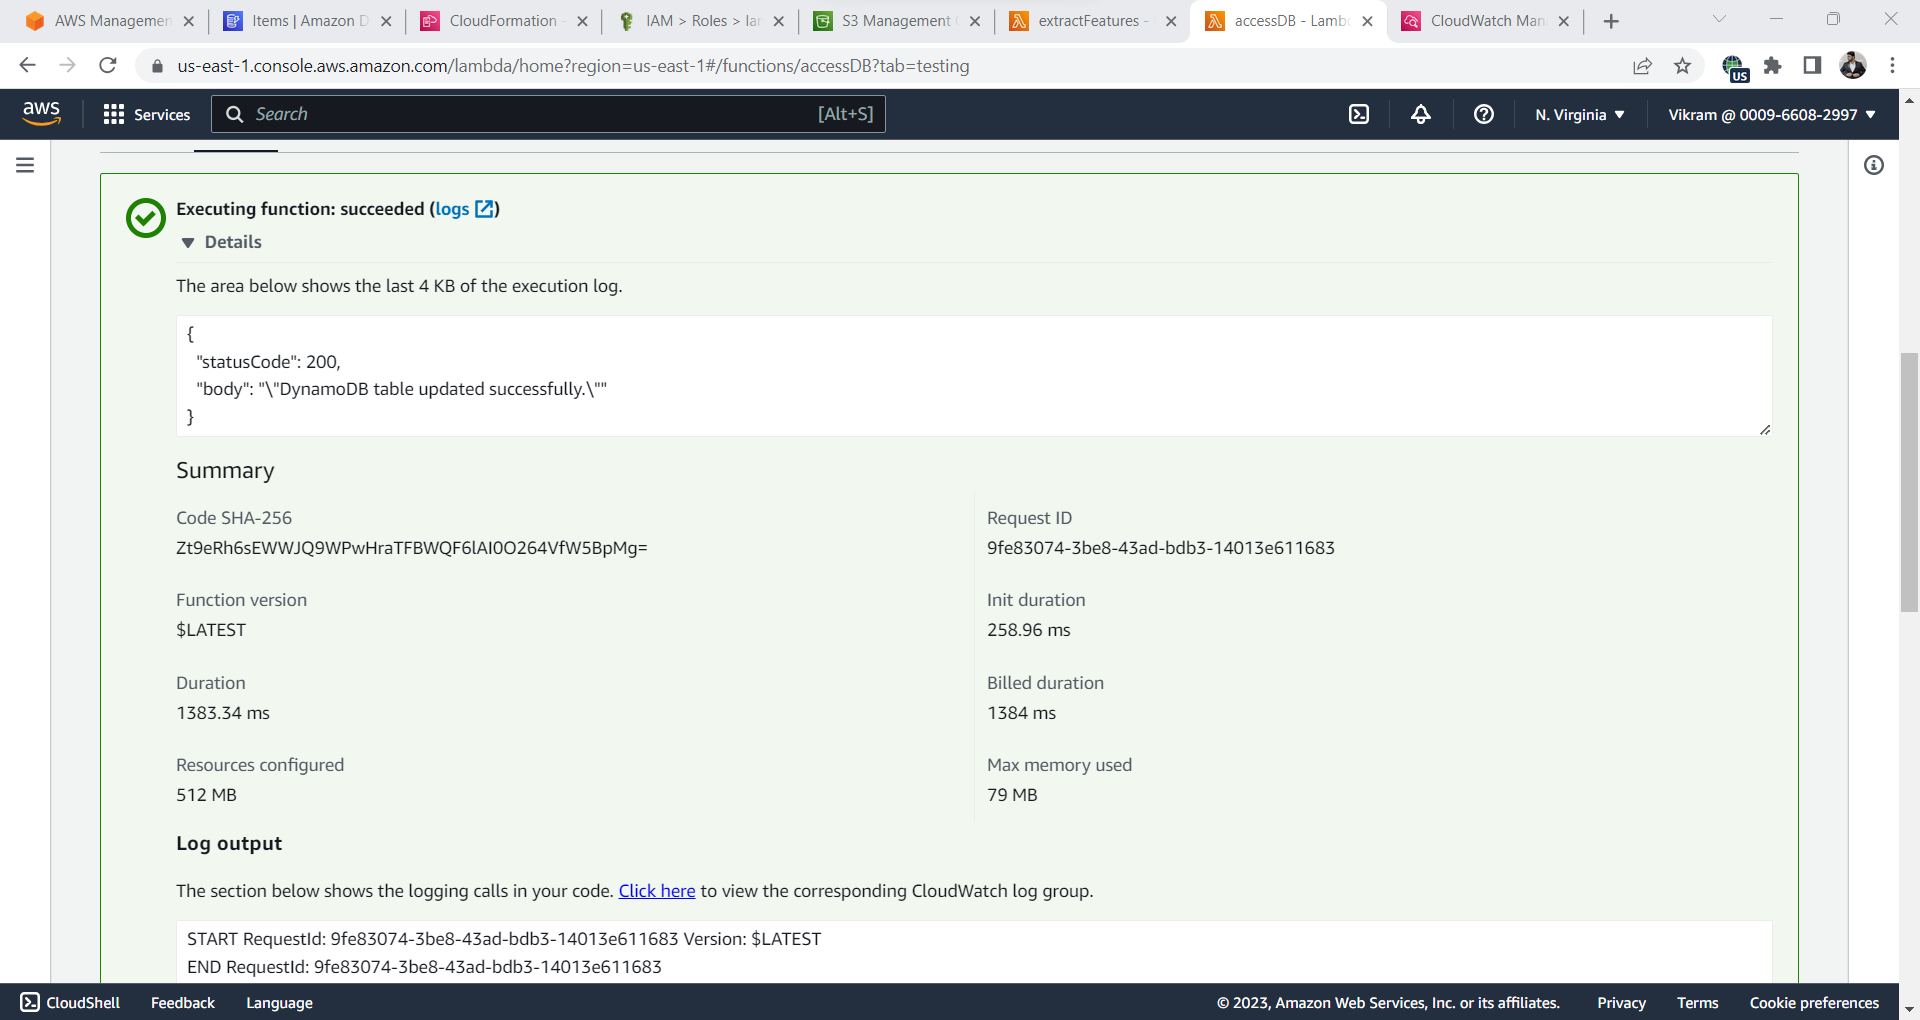
\includegraphics[scale=1, width=15cm,height=7.5cm]{PROBLEM 2/Screenshots/8.2 accessDB unit test.png}}
    \caption{\textbf{\textit{accessDB lambda unit test}}}
    \label{fig:}
\end{figure}

\begin{figure}[htp]
    \centering
    \fbox{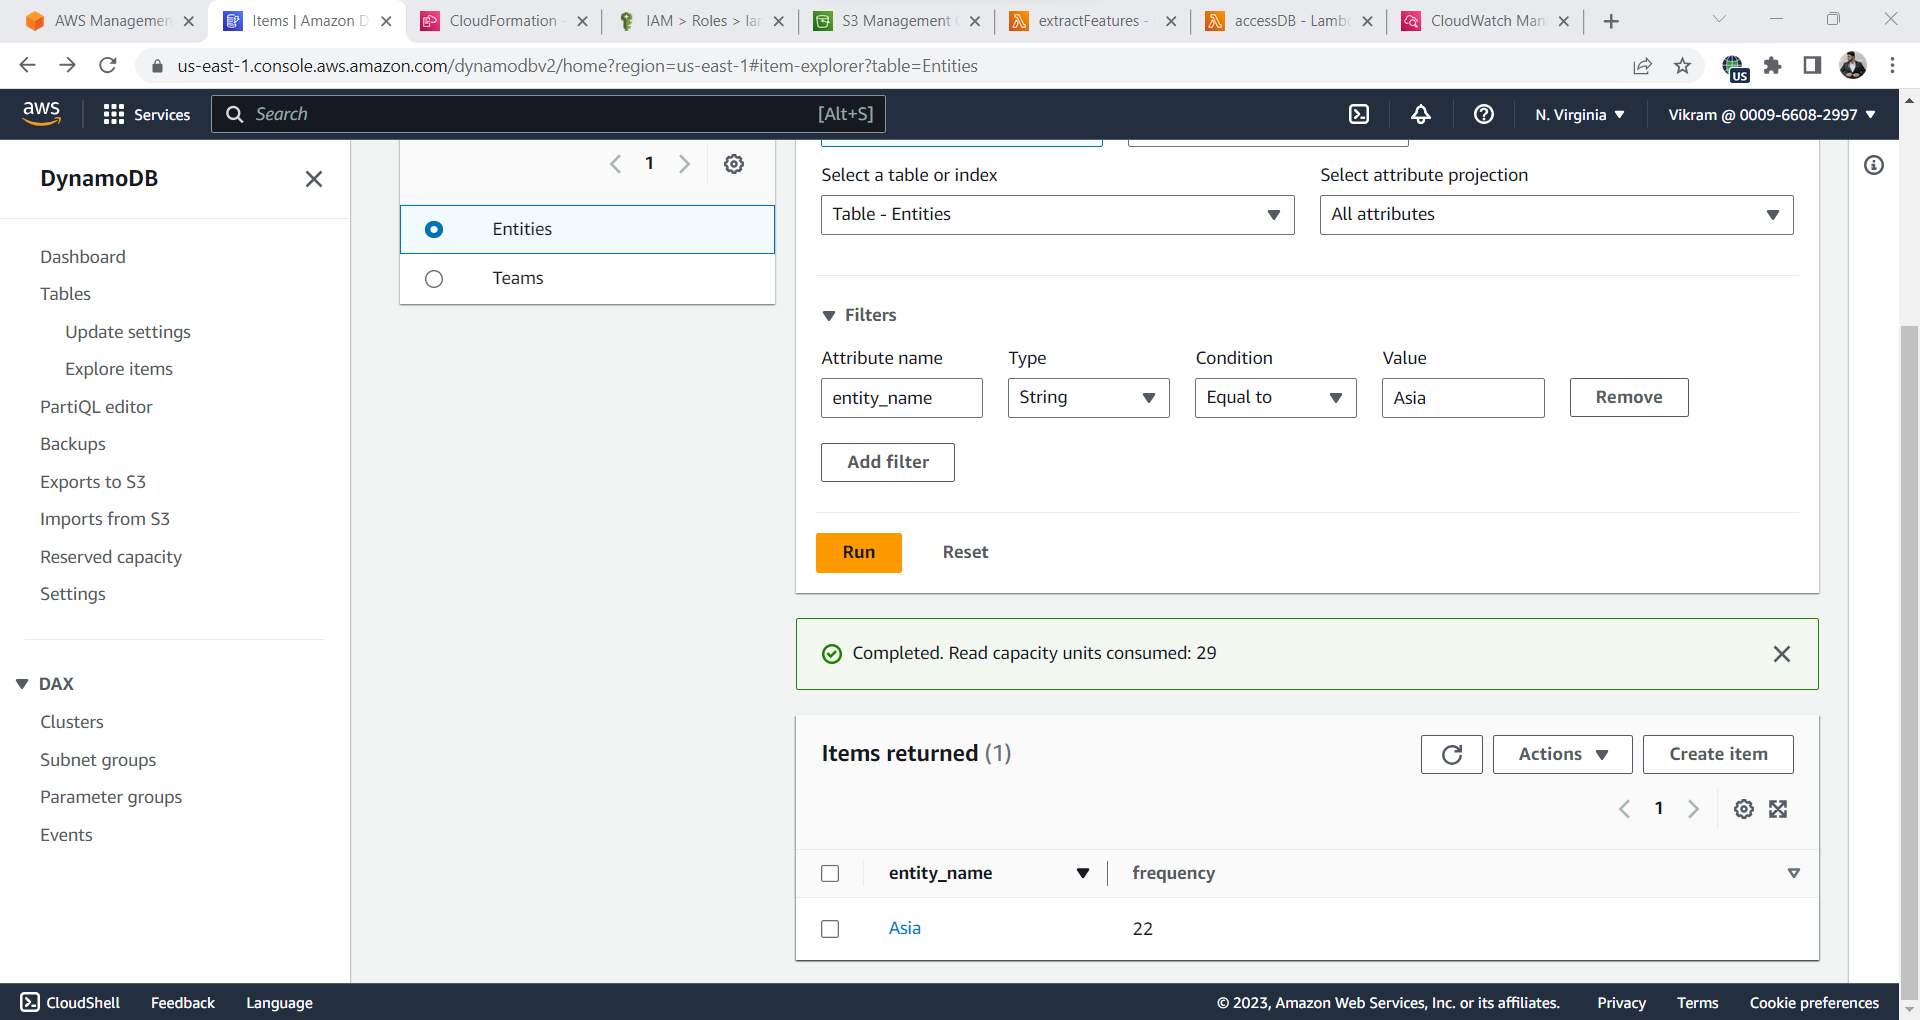
\includegraphics[scale=1, width=15cm,height=7.5cm]{PROBLEM 2/Screenshots/9.1 query entity_name=Asia.png}}
    \caption{\textbf{\textit{Sample query with entity_name="Asia"}}}
    \label{fig:}
\end{figure}

\newpage
\section{Testing}
\subsection{Procedure}
\begin{enumerate}
    \item Created a new file named '000.txt' with the following content:
  \begin{mdframed}[linewidth=1pt]
\begin{verbatim}
sample txt file for testing purposes:

all lowercase   
                : ggggggg
all uppercase   
                : GGGGGGG
Starting uppercase, 
other lowercase 
                : Ggggggg
numbers         
                : 0000000
\end{verbatim}
\end{mdframed}

    \item Named entities in this file are: GGGGGGG, Starting, Ggggggg
    \item Uploaded the file via CLI.
    \item Verfied the file upload in bucket sample-data-b00936916 on console.
    \item Verified the triggering of events by checking the logs of lambda functions: extractFeatures, accessDB.
    \item Verified the file contents of generated '000ne.txt' file in bucket tags-b00936916 on console, by downloading the file.
    \item Queried the extracted entities in DynamoDB and verified their frequency.
\end{enumerate}

\newpage
\subsection{Screenshots}

\begin{figure}[htp]
    \centering
    \fbox{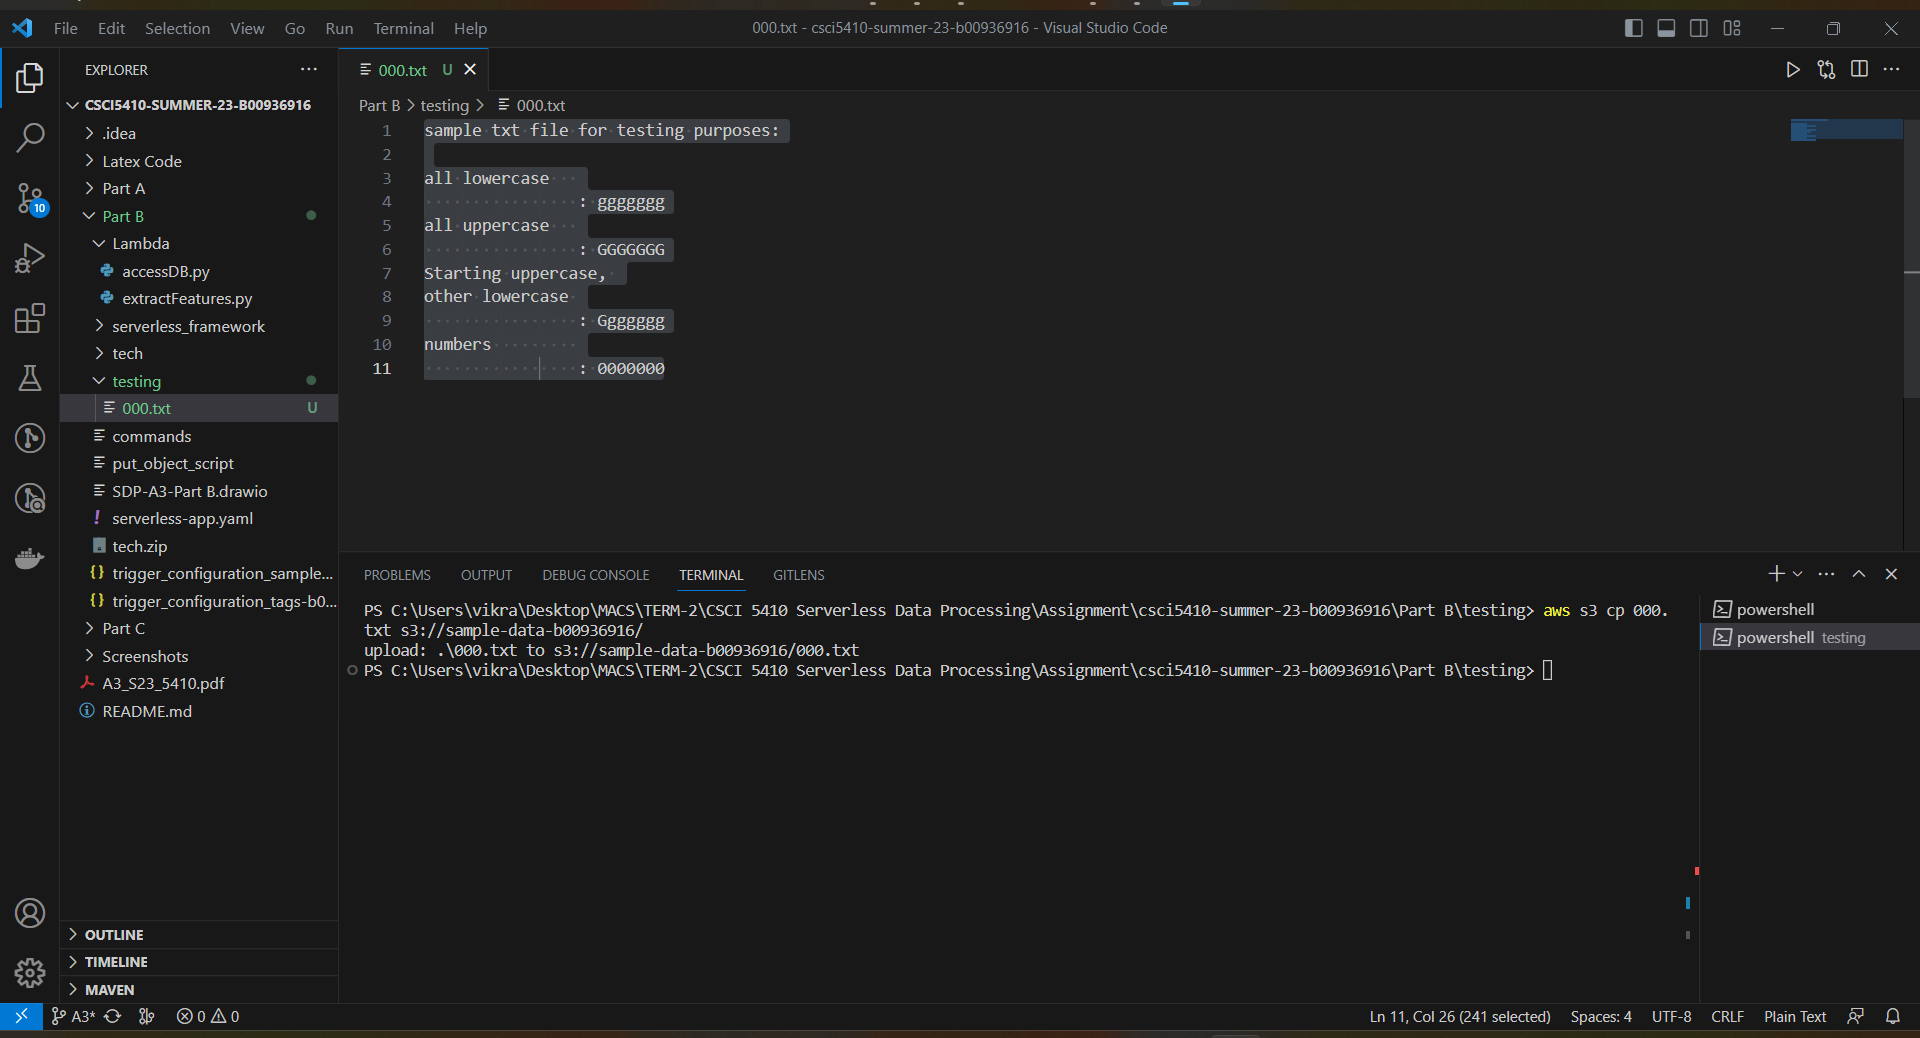
\includegraphics[scale=1, width=15cm,height=6.5cm]{PROBLEM 2/Testing/1. upload 000.txt via CLI.png}}
    \caption{\textbf{\textit{Upload 000.txt via CLI}}}
    \label{fig:}
\end{figure}

\begin{figure}[htp]
    \centering
    \fbox{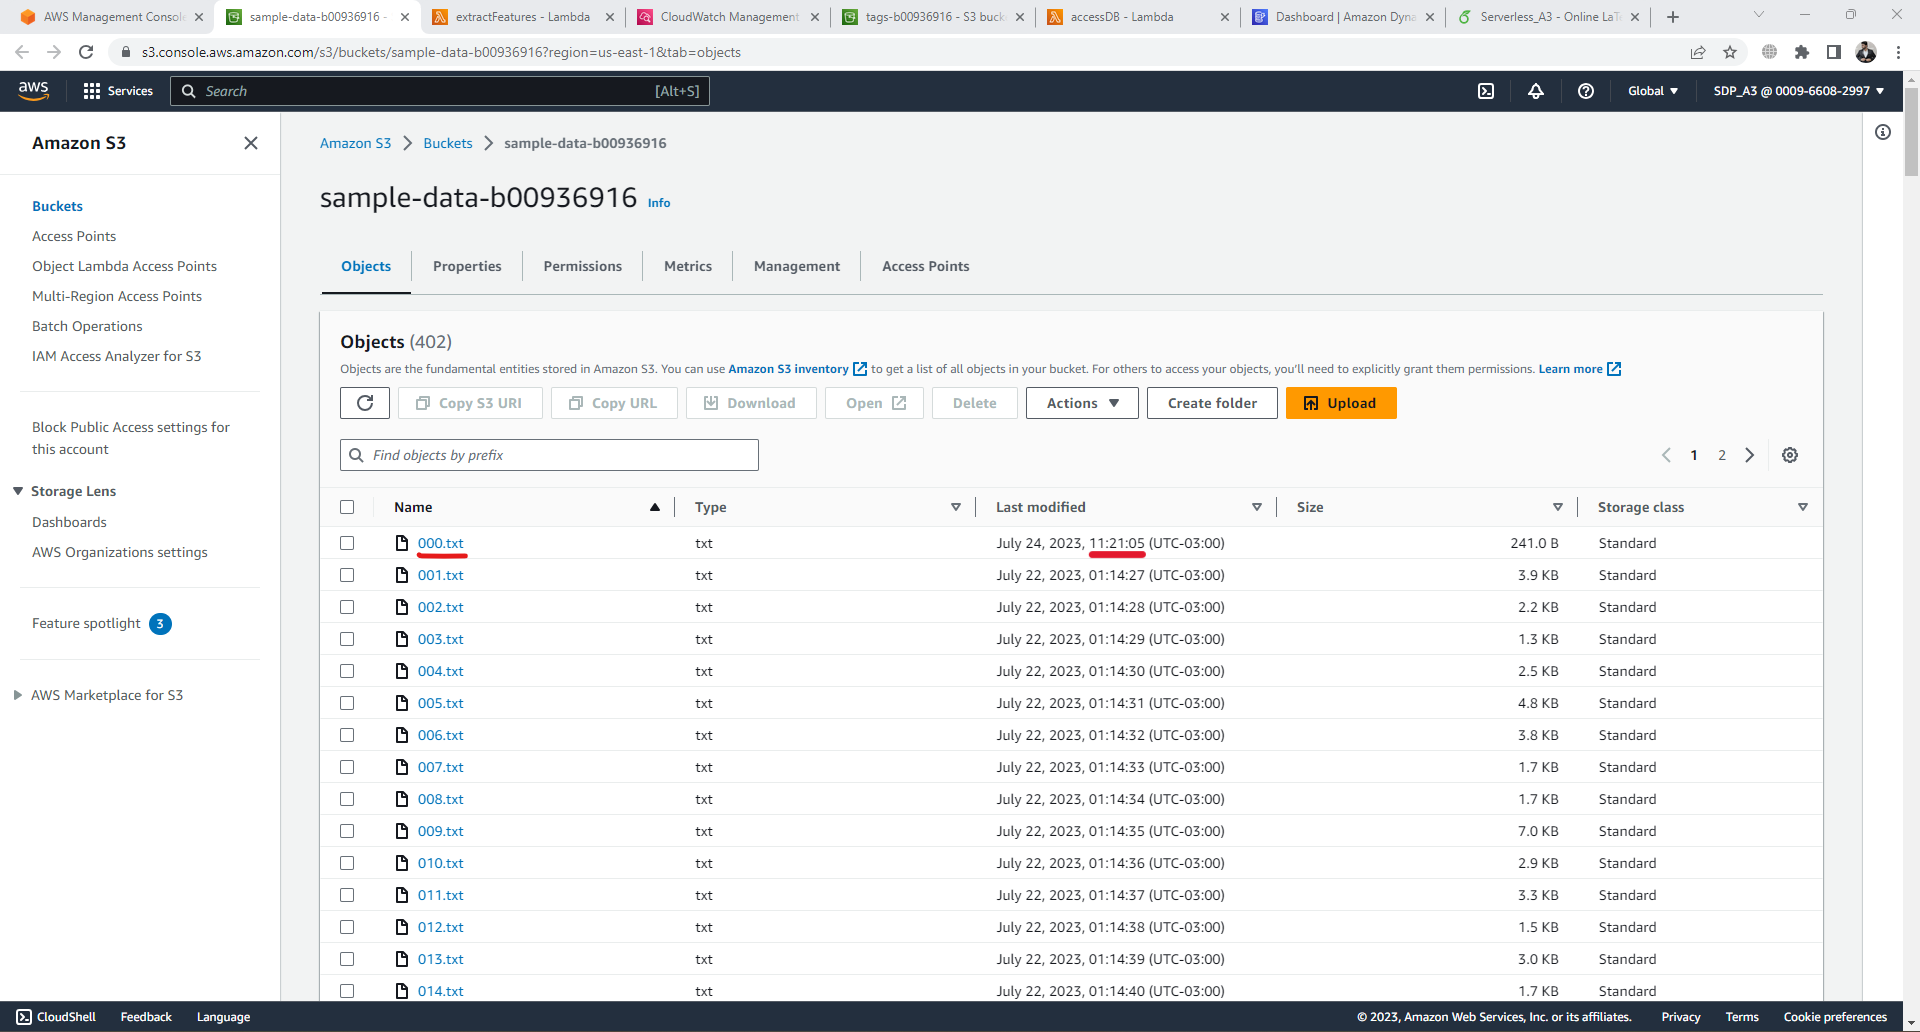
\includegraphics[scale=1, width=15cm,height=6.5cm]{PROBLEM 2/Testing/1.1 file uploaded in bucket sample-data-b00936916 - console.png}}
    \caption{\textbf{\textit{File uploaded in bucket sample-data-b00936916 - console}}}
    \label{fig:}
\end{figure}

\begin{figure}[htp]
    \centering
    \fbox{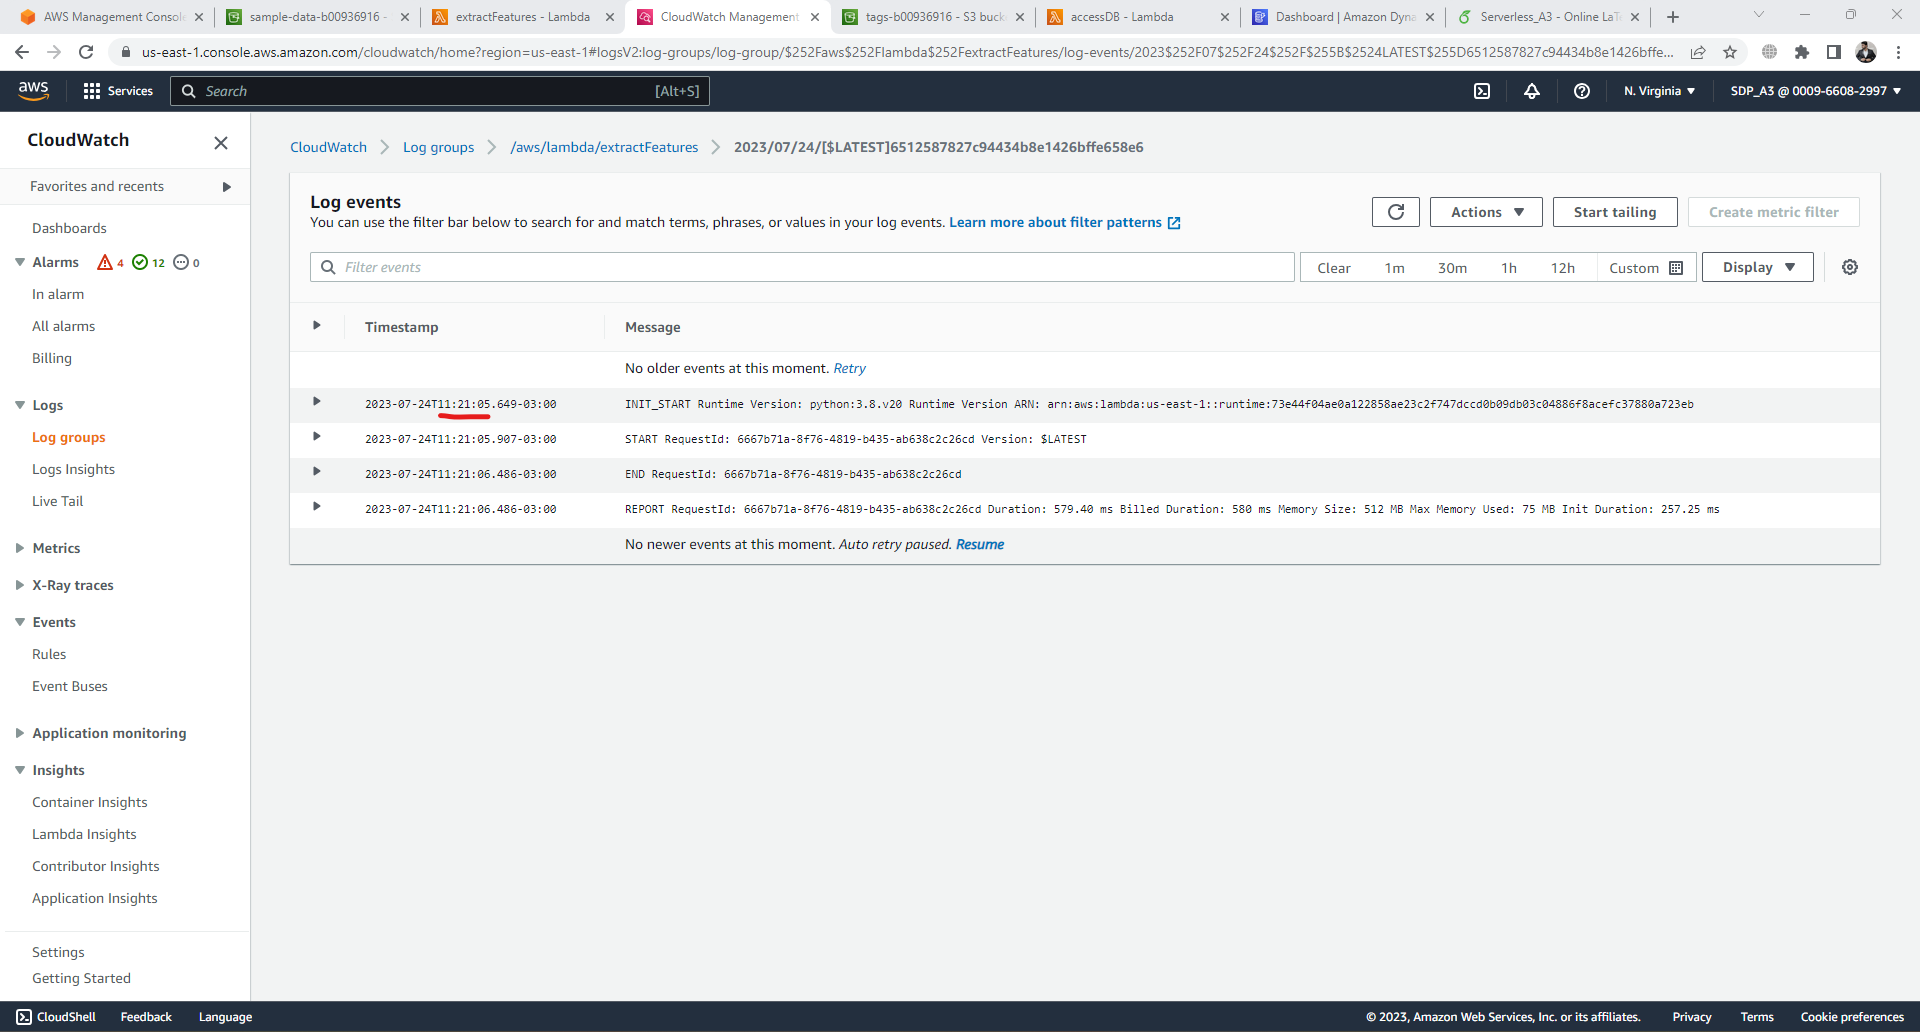
\includegraphics[scale=1, width=15cm,height=7.5cm]{PROBLEM 2/Testing/2. logs in extractFeatures lambda - notice the timestamp.png}}
    \caption{\textbf{\textit{Logs in extractFeatures lambda - notice the timestamp}}}
    \label{fig:}
\end{figure}


\begin{figure}[htp]
    \centering
    \fbox{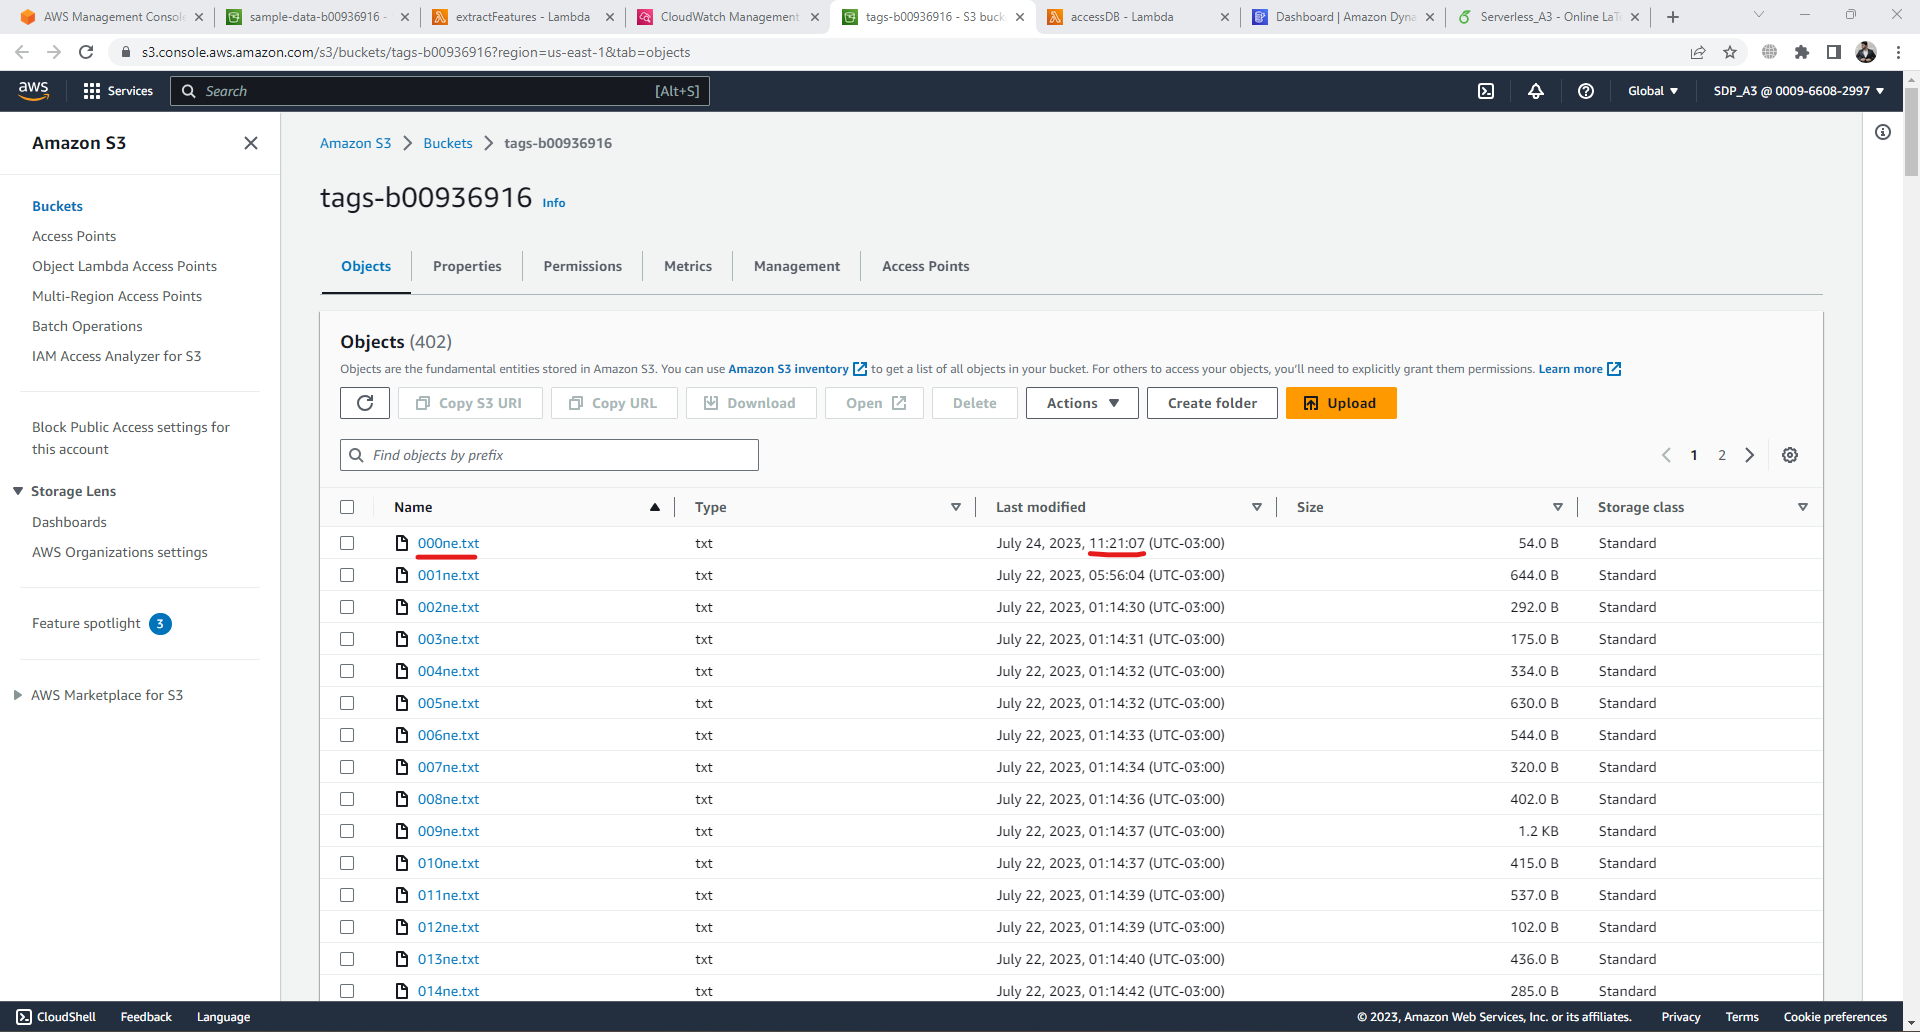
\includegraphics[scale=1, width=15cm,height=7.5cm]{PROBLEM 2/Testing/3. 000ne.txt file in bucket tags-b00936916.png}}
    \caption{\textbf{\textit{000ne.txt file in bucket tags-b00936916}}}
    \label{fig:}
\end{figure}

\begin{figure}[htp]
    \centering
    \fbox{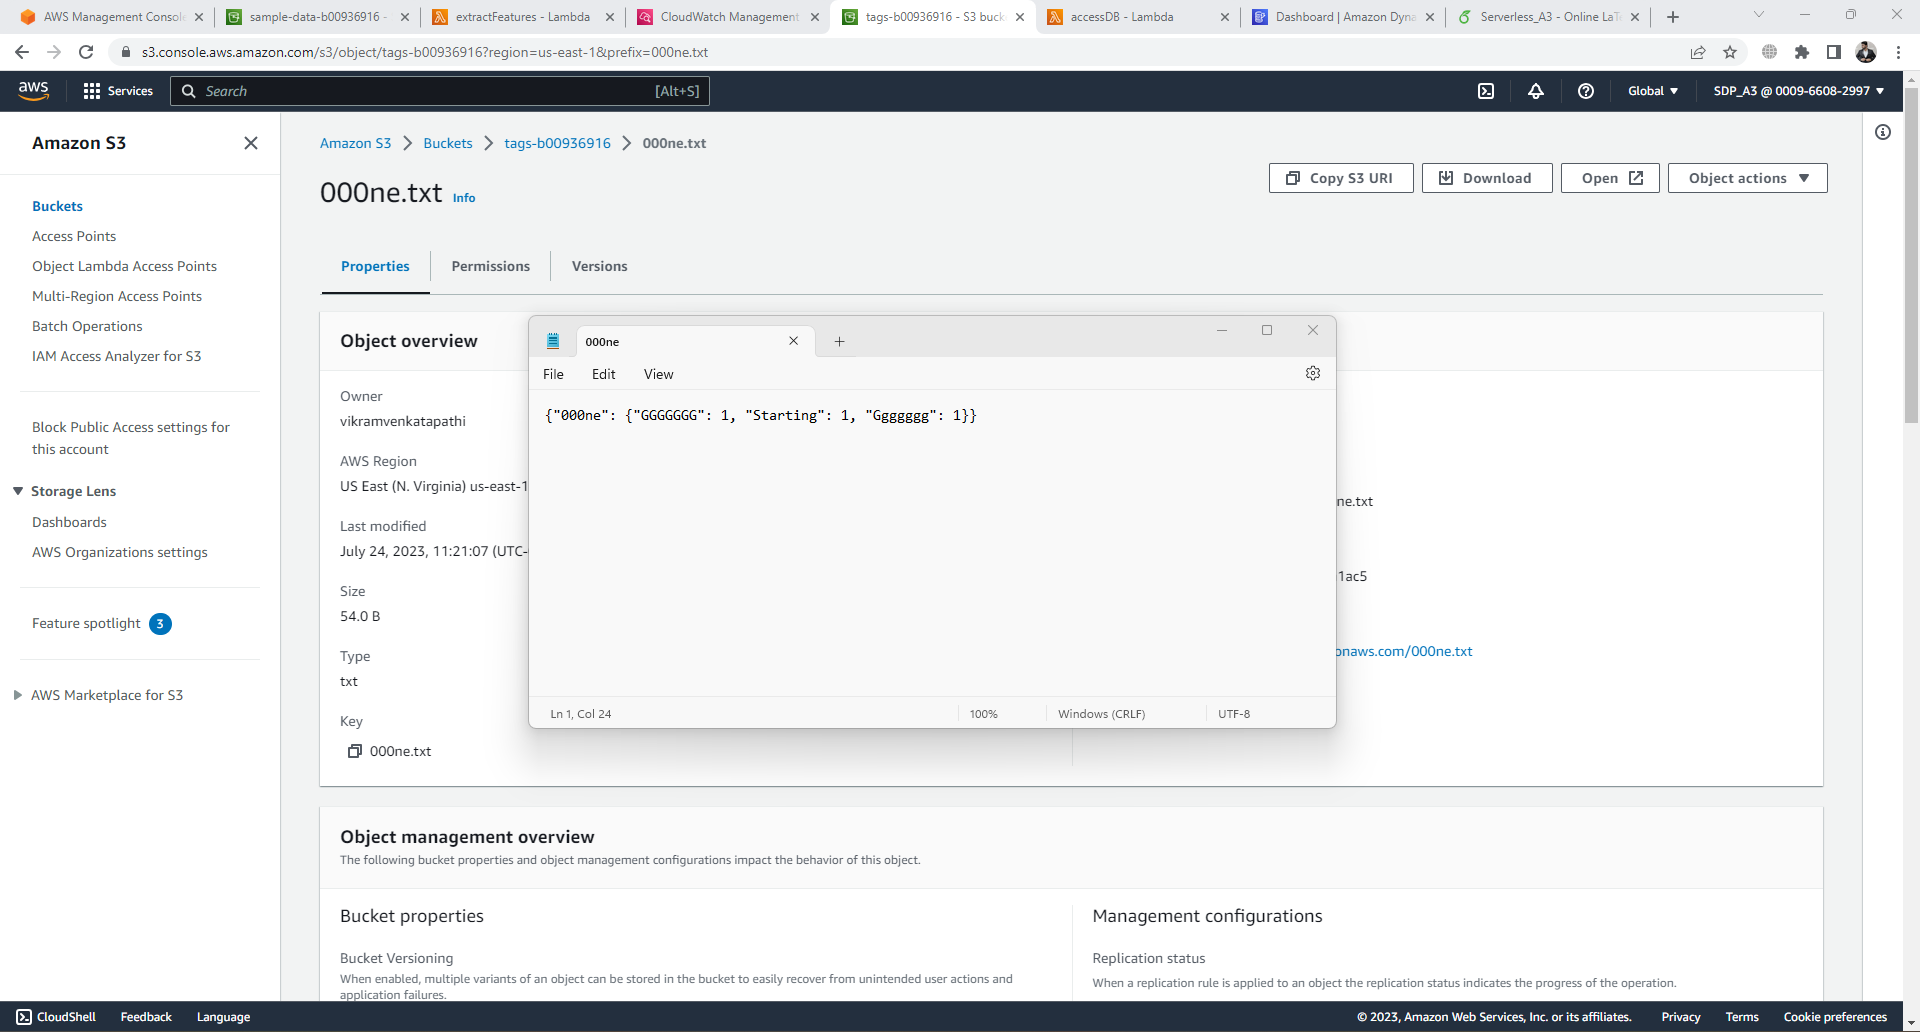
\includegraphics[scale=1, width=15cm,height=7.5cm]{PROBLEM 2/Testing/4. 000ne.txt file contents - with entities.png}}
    \caption{\textbf{\textit{000ne.txt file contents - with named entities}}}
    \label{fig:}
\end{figure}

\begin{figure}[htp]
    \centering
    \fbox{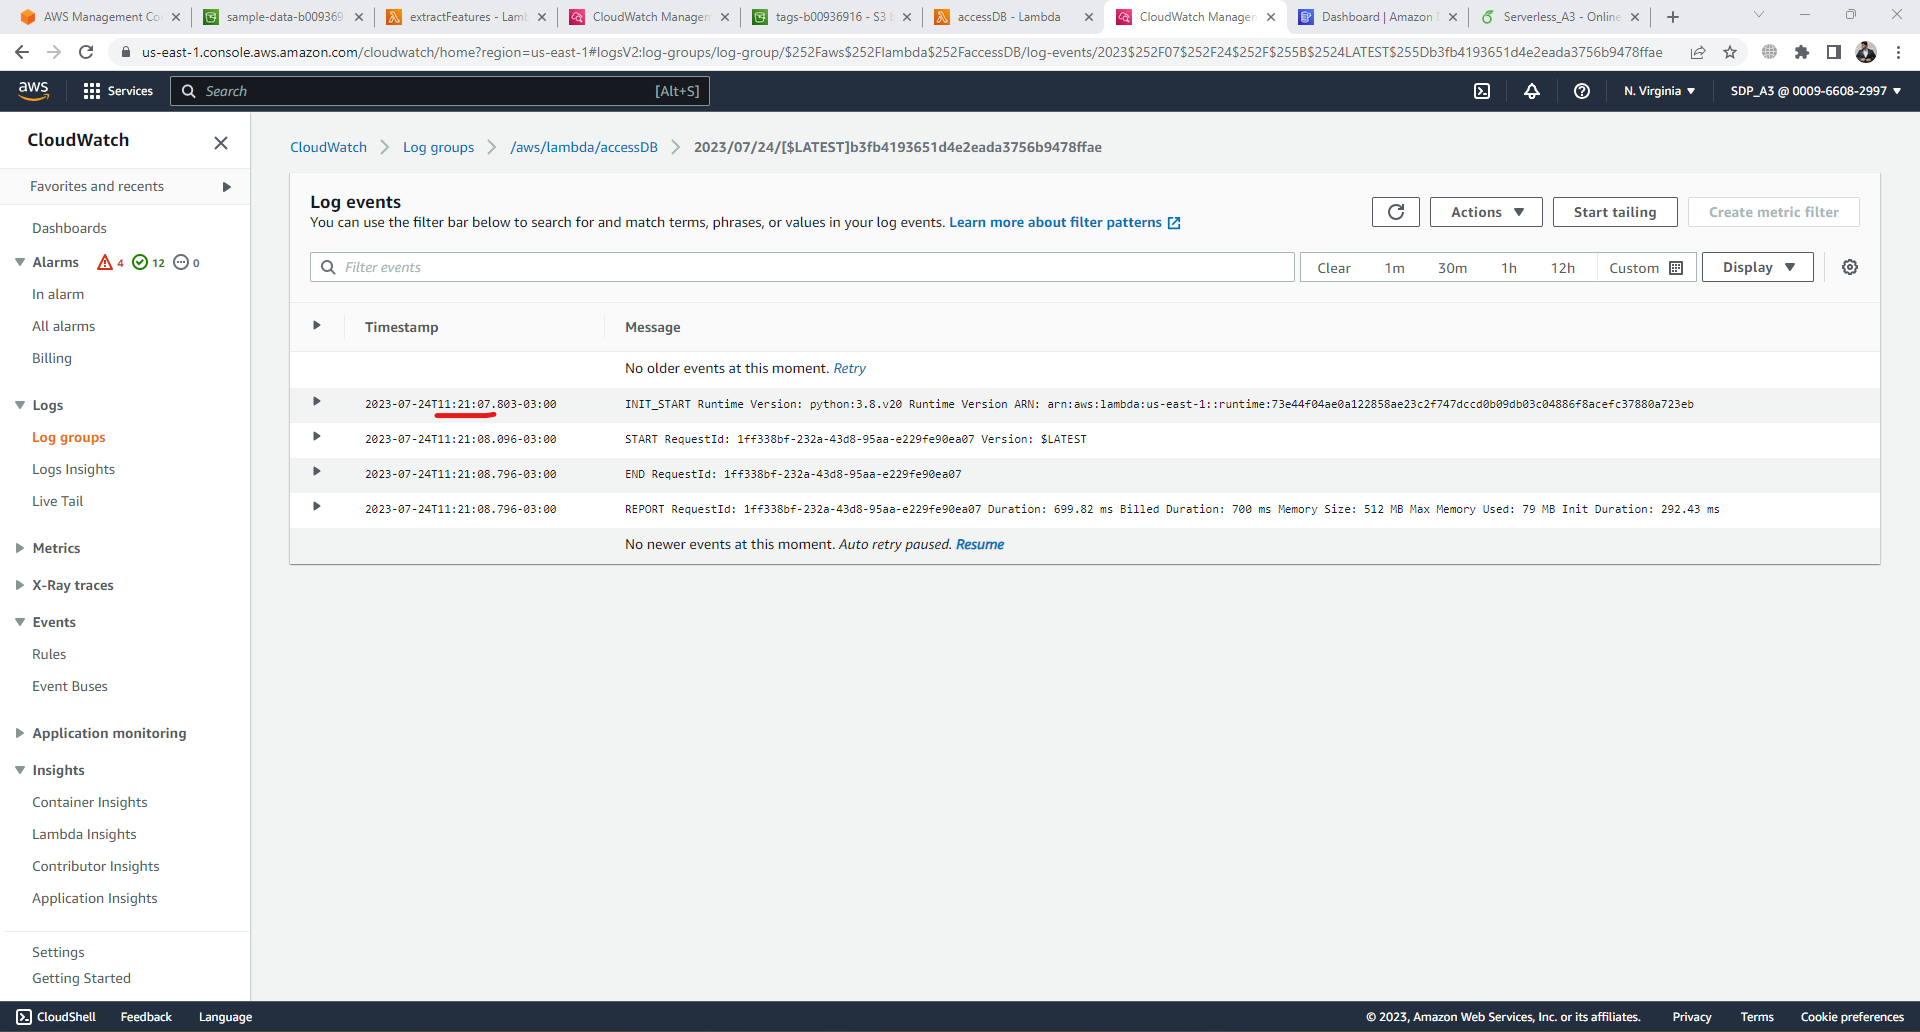
\includegraphics[scale=1, width=15cm,height=7.5cm]{PROBLEM 2/Testing/5. logs in accessDB lambda - notice the timestamp.png}}
    \caption{\textbf{\textit{Logs in accessDB lambda - notice the timestamp}}}
    \label{fig:}
\end{figure}

\begin{figure}[htp]
    \centering
    \fbox{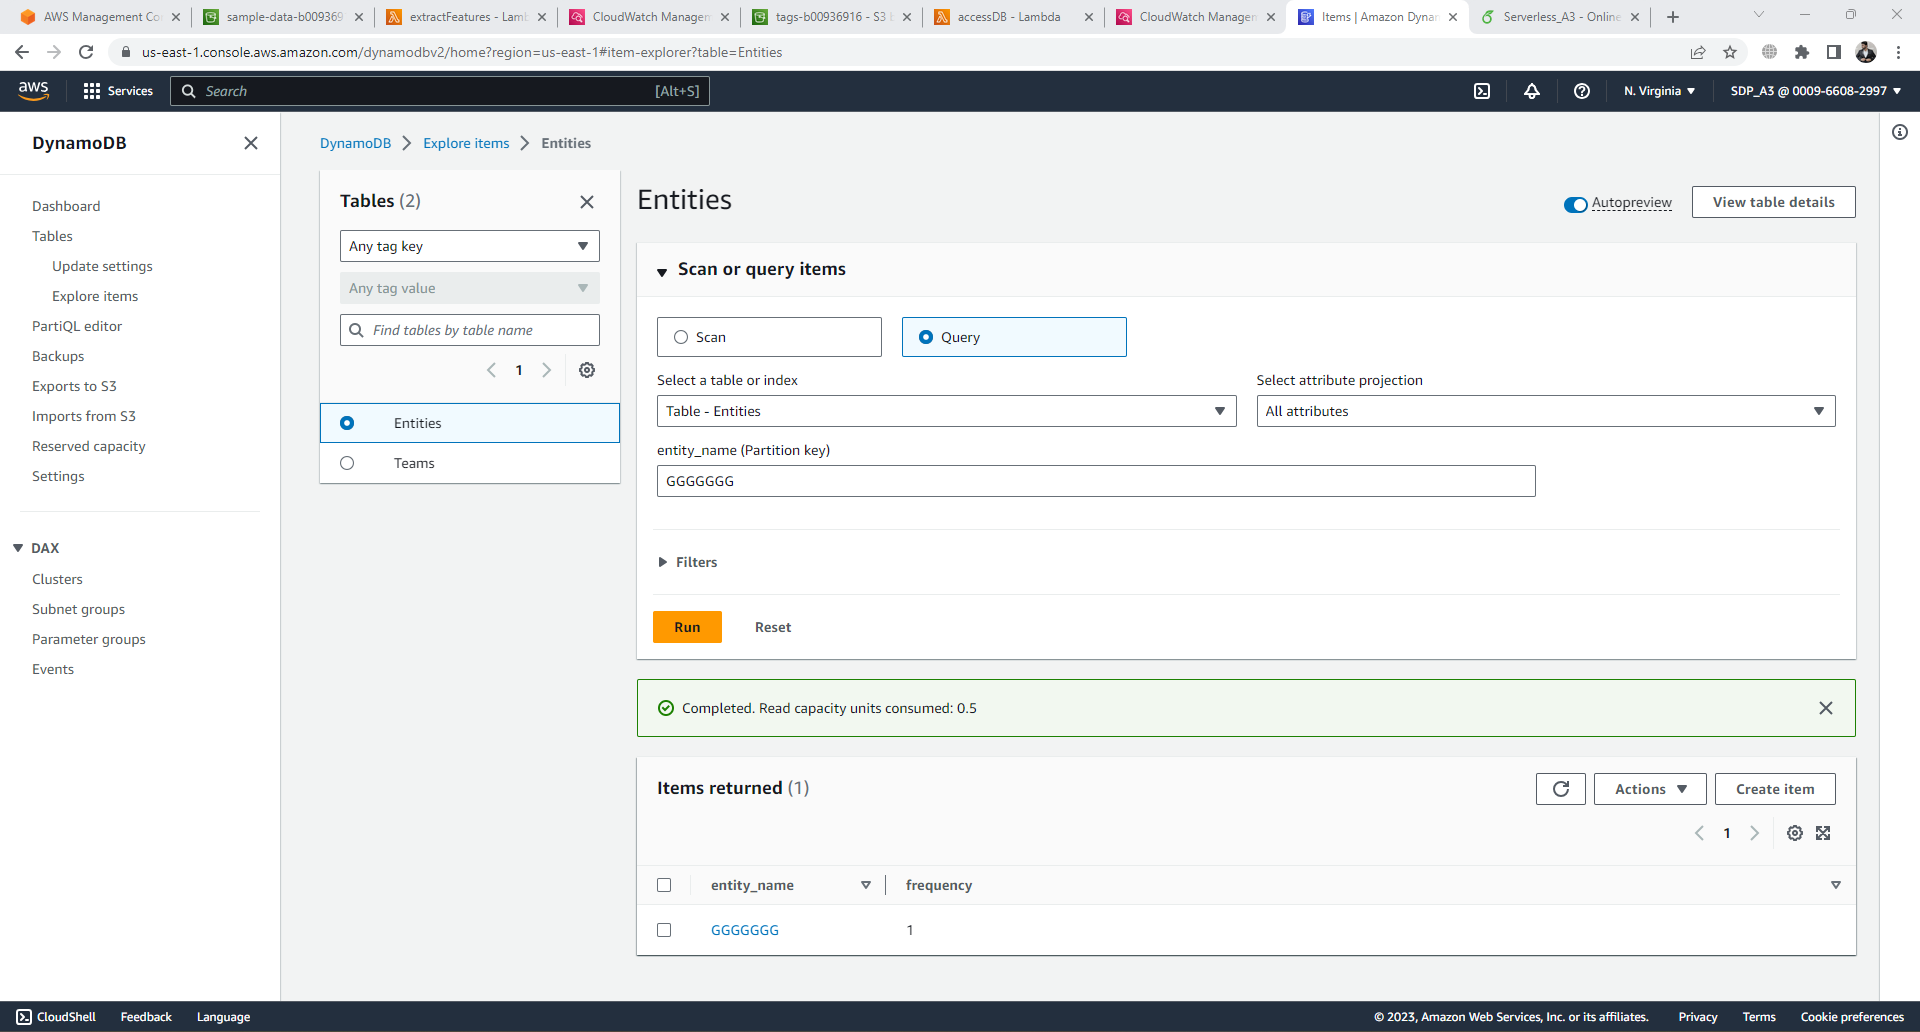
\includegraphics[scale=1, width=15cm,height=7.5cm]{PROBLEM 2/Testing/6.1 Query - GGGGGGG - frequency=1 in table .png}}
    \caption{\textbf{\textit{Query : entity\_name=GGGGGGG, frequency=1 in table }}}
    \label{fig:}
\end{figure}

\begin{figure}[htp]
    \centering
    \fbox{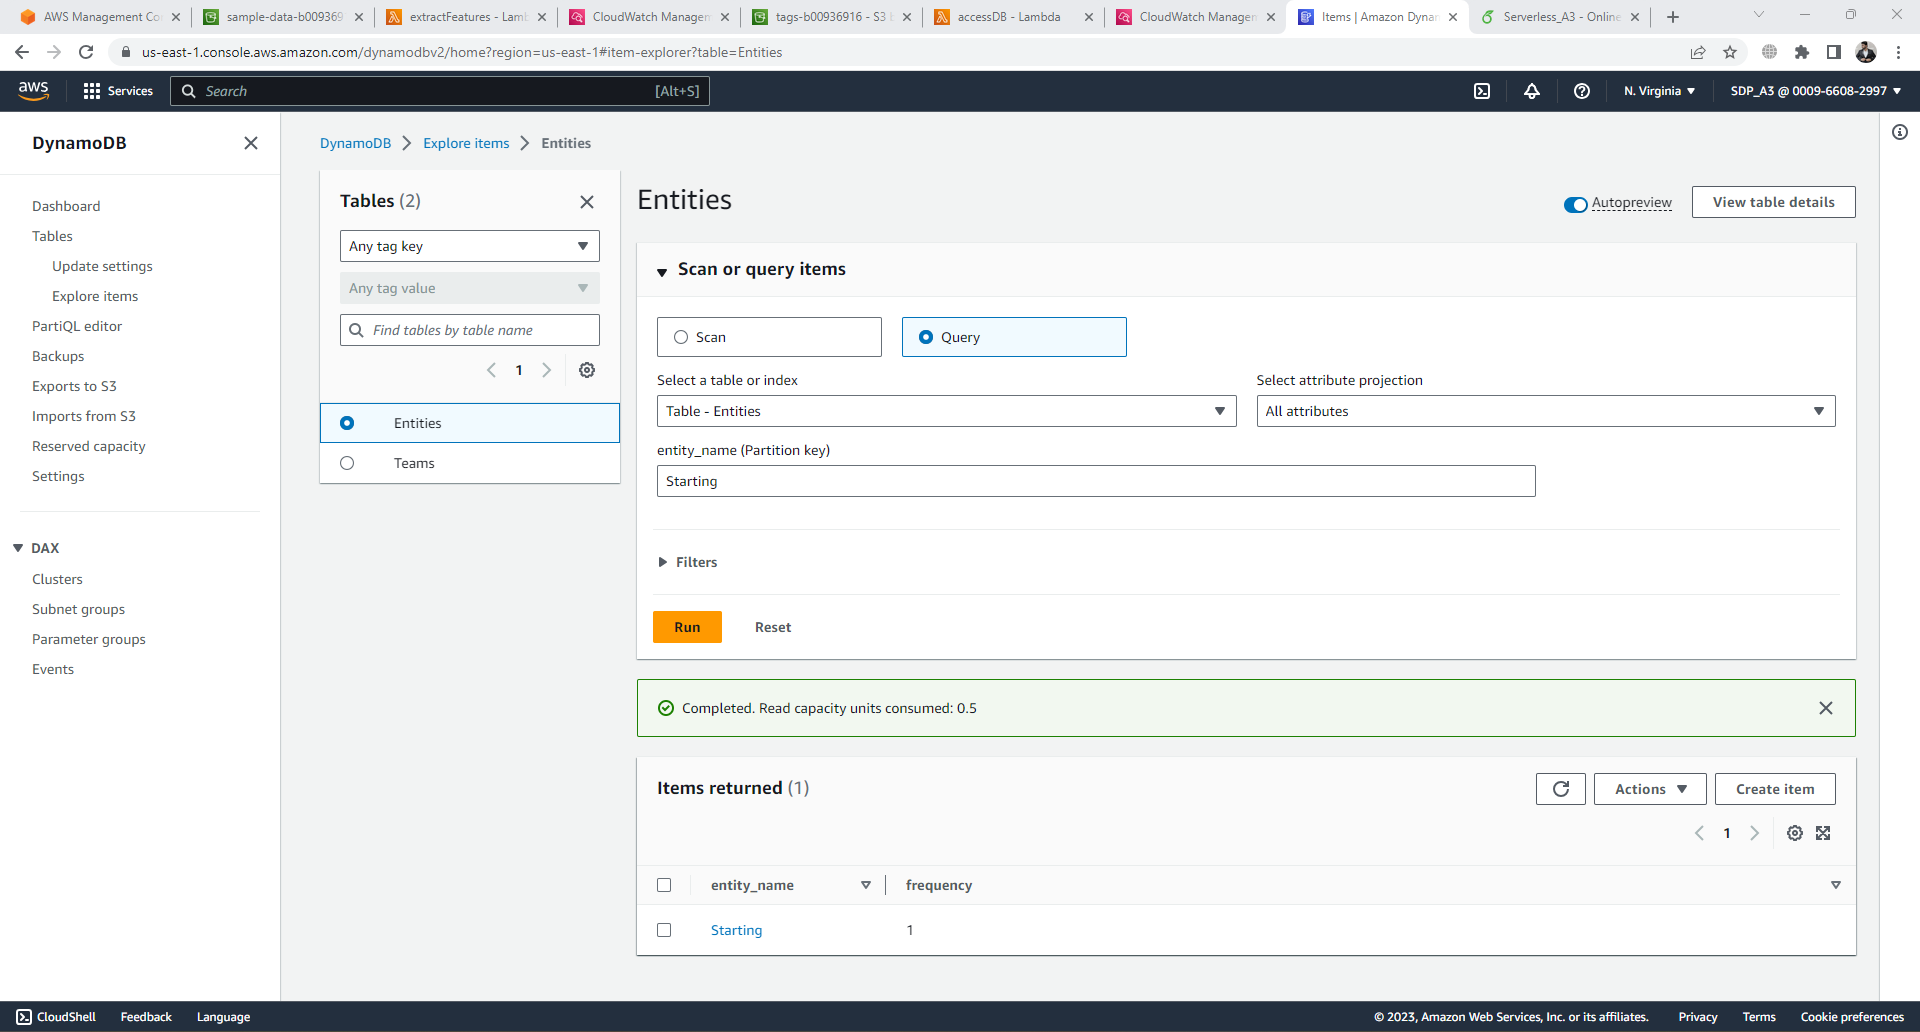
\includegraphics[scale=1, width=15cm,height=7.5cm]{PROBLEM 2/Testing/6.2 Query - Starting frequency=1 in table .png}}
    \caption{\textbf{\textit{Query : entity\_name=Starting, frequency=1 in table }}}
    \label{fig:}
\end{figure}

\begin{figure}[htp]
    \centering
    \fbox{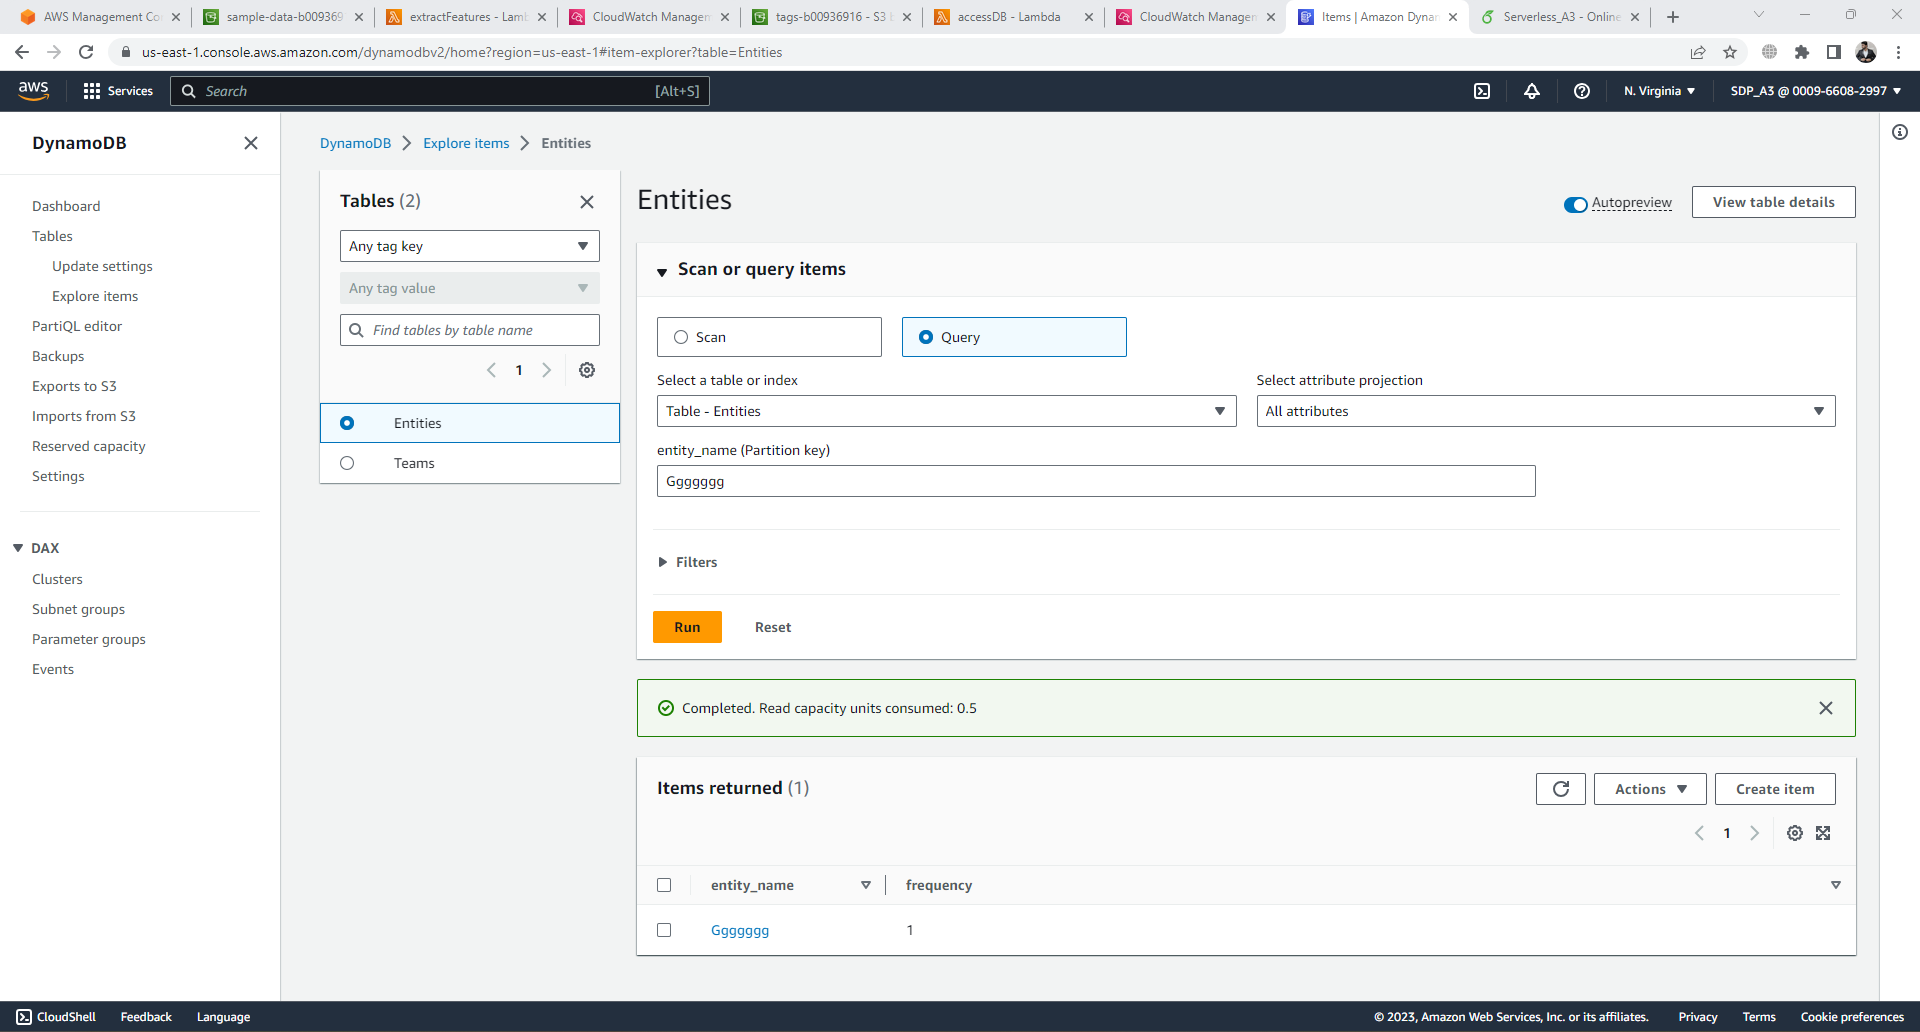
\includegraphics[scale=1, width=15cm,height=7.5cm]{PROBLEM 2/Testing/6.3 Query - Ggggggg - frequency=1 in table .png}}
    \caption{\textbf{\textit{Query : entity\_name=Ggggggg, frequency=1 in table}}}
    \label{fig:}
\end{figure}

\begin{figure}[htp]
    \centering
    \fbox{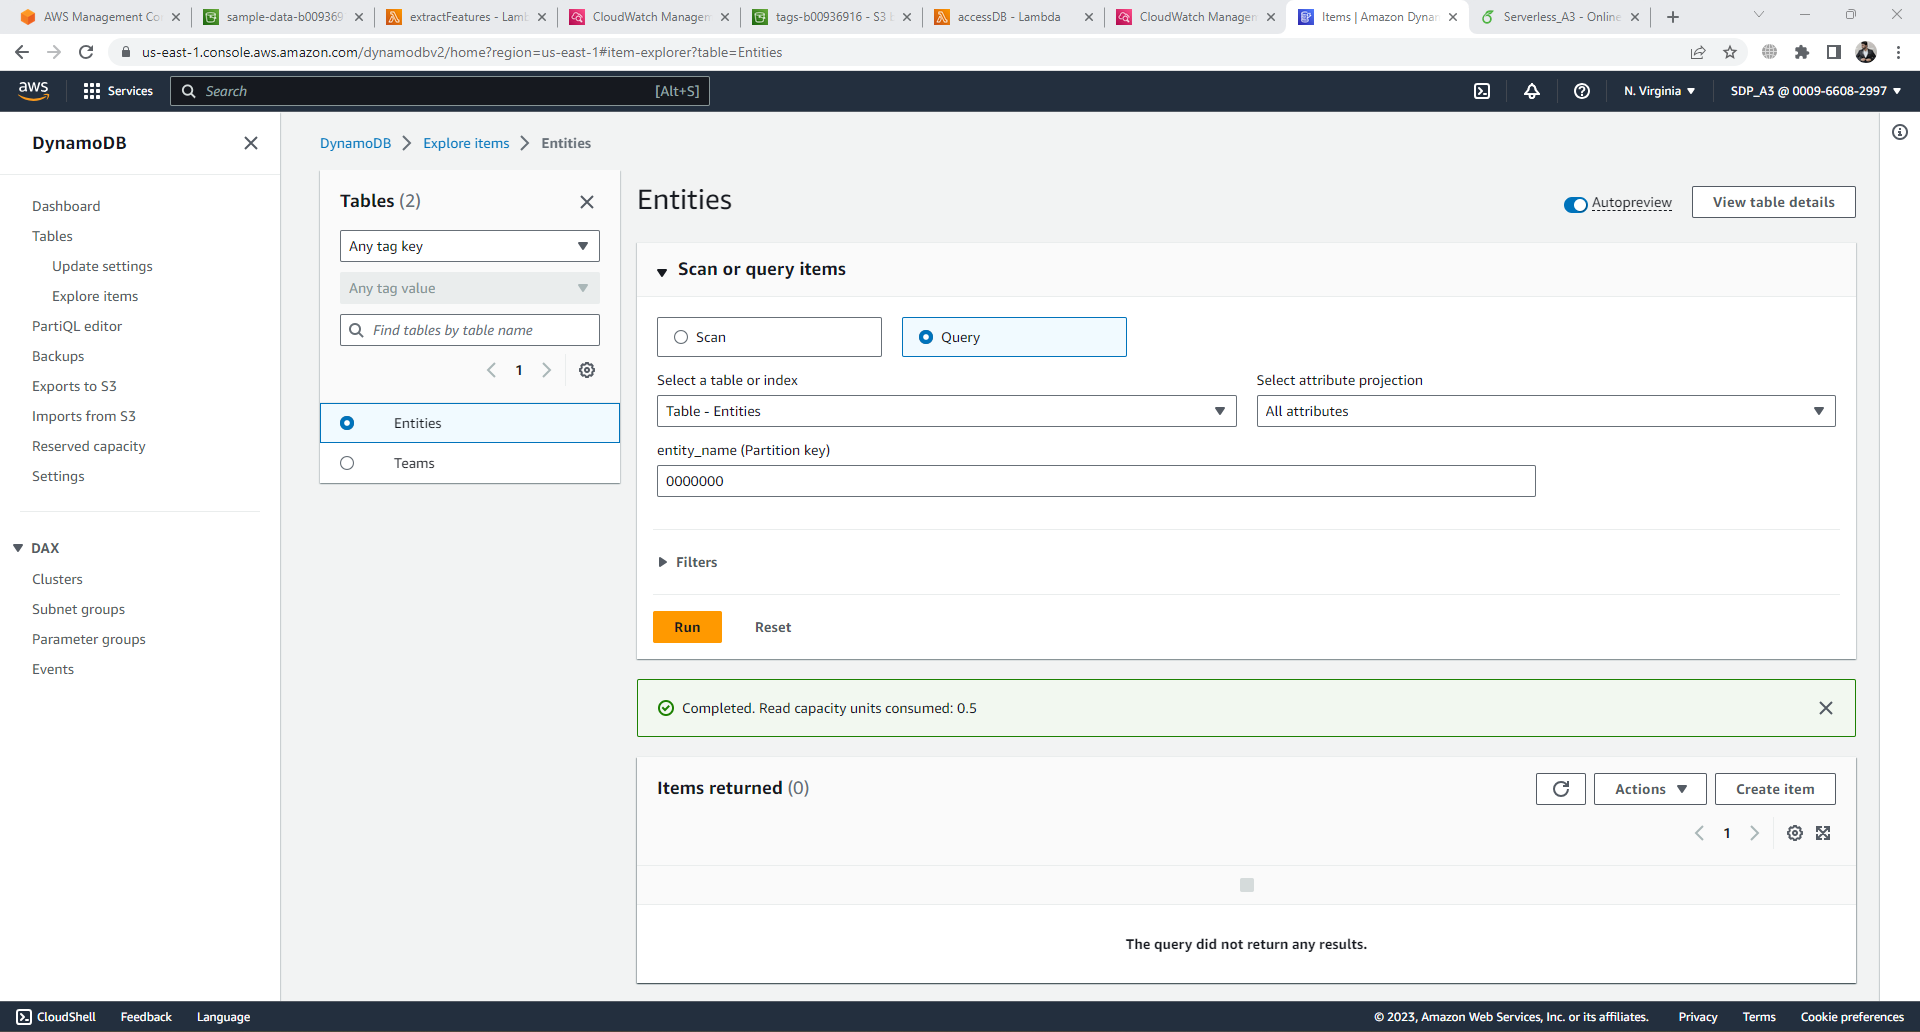
\includegraphics[scale=1, width=15cm,height=7.5cm]{PROBLEM 2/Testing/6.4 Query - 0000000- frequency=0 in table .png}}
    \caption{\textbf{\textit{Query : entity\_name=0000000, frequency=0 in table}}}
    \label{fig:}
\end{figure}


% \begin{figure}[htp]
%     \centering
%     \fbox{\includegraphics[scale=1, width=15cm,height=7.5cm]{PROBLEM 2/}}
%     \caption{\textbf{\textit{}}}
%     \label{fig:}
% \end{figure}

\newpage
\newpage